\documentclass[11pt,]{article}
\usepackage[left=1in,top=1in,right=1in,bottom=1in]{geometry}
\newcommand*{\authorfont}{\fontfamily{phv}\selectfont}
\usepackage[]{mathpazo}


  \usepackage[T1]{fontenc}
  \usepackage[utf8]{inputenc}



\usepackage{abstract}
\renewcommand{\abstractname}{}    % clear the title
\renewcommand{\absnamepos}{empty} % originally center

\renewenvironment{abstract}
 {{%
    \setlength{\leftmargin}{0mm}
    \setlength{\rightmargin}{\leftmargin}%
  }%
  \relax}
 {\endlist}

\makeatletter
\def\@maketitle{%
  \newpage
%  \null
%  \vskip 2em%
%  \begin{center}%
  \let \footnote \thanks
    {\fontsize{18}{20}\selectfont\raggedright  \setlength{\parindent}{0pt} \@title \par}%
}
%\fi
\makeatother




\setcounter{secnumdepth}{3}

\usepackage{color}
\usepackage{fancyvrb}
\newcommand{\VerbBar}{|}
\newcommand{\VERB}{\Verb[commandchars=\\\{\}]}
\DefineVerbatimEnvironment{Highlighting}{Verbatim}{commandchars=\\\{\}}
% Add ',fontsize=\small' for more characters per line
\usepackage{framed}
\definecolor{shadecolor}{RGB}{248,248,248}
\newenvironment{Shaded}{\begin{snugshade}}{\end{snugshade}}
\newcommand{\KeywordTok}[1]{\textcolor[rgb]{0.13,0.29,0.53}{\textbf{#1}}}
\newcommand{\DataTypeTok}[1]{\textcolor[rgb]{0.13,0.29,0.53}{#1}}
\newcommand{\DecValTok}[1]{\textcolor[rgb]{0.00,0.00,0.81}{#1}}
\newcommand{\BaseNTok}[1]{\textcolor[rgb]{0.00,0.00,0.81}{#1}}
\newcommand{\FloatTok}[1]{\textcolor[rgb]{0.00,0.00,0.81}{#1}}
\newcommand{\ConstantTok}[1]{\textcolor[rgb]{0.00,0.00,0.00}{#1}}
\newcommand{\CharTok}[1]{\textcolor[rgb]{0.31,0.60,0.02}{#1}}
\newcommand{\SpecialCharTok}[1]{\textcolor[rgb]{0.00,0.00,0.00}{#1}}
\newcommand{\StringTok}[1]{\textcolor[rgb]{0.31,0.60,0.02}{#1}}
\newcommand{\VerbatimStringTok}[1]{\textcolor[rgb]{0.31,0.60,0.02}{#1}}
\newcommand{\SpecialStringTok}[1]{\textcolor[rgb]{0.31,0.60,0.02}{#1}}
\newcommand{\ImportTok}[1]{#1}
\newcommand{\CommentTok}[1]{\textcolor[rgb]{0.56,0.35,0.01}{\textit{#1}}}
\newcommand{\DocumentationTok}[1]{\textcolor[rgb]{0.56,0.35,0.01}{\textbf{\textit{#1}}}}
\newcommand{\AnnotationTok}[1]{\textcolor[rgb]{0.56,0.35,0.01}{\textbf{\textit{#1}}}}
\newcommand{\CommentVarTok}[1]{\textcolor[rgb]{0.56,0.35,0.01}{\textbf{\textit{#1}}}}
\newcommand{\OtherTok}[1]{\textcolor[rgb]{0.56,0.35,0.01}{#1}}
\newcommand{\FunctionTok}[1]{\textcolor[rgb]{0.00,0.00,0.00}{#1}}
\newcommand{\VariableTok}[1]{\textcolor[rgb]{0.00,0.00,0.00}{#1}}
\newcommand{\ControlFlowTok}[1]{\textcolor[rgb]{0.13,0.29,0.53}{\textbf{#1}}}
\newcommand{\OperatorTok}[1]{\textcolor[rgb]{0.81,0.36,0.00}{\textbf{#1}}}
\newcommand{\BuiltInTok}[1]{#1}
\newcommand{\ExtensionTok}[1]{#1}
\newcommand{\PreprocessorTok}[1]{\textcolor[rgb]{0.56,0.35,0.01}{\textit{#1}}}
\newcommand{\AttributeTok}[1]{\textcolor[rgb]{0.77,0.63,0.00}{#1}}
\newcommand{\RegionMarkerTok}[1]{#1}
\newcommand{\InformationTok}[1]{\textcolor[rgb]{0.56,0.35,0.01}{\textbf{\textit{#1}}}}
\newcommand{\WarningTok}[1]{\textcolor[rgb]{0.56,0.35,0.01}{\textbf{\textit{#1}}}}
\newcommand{\AlertTok}[1]{\textcolor[rgb]{0.94,0.16,0.16}{#1}}
\newcommand{\ErrorTok}[1]{\textcolor[rgb]{0.64,0.00,0.00}{\textbf{#1}}}
\newcommand{\NormalTok}[1]{#1}
\usepackage{longtable,booktabs}

\usepackage{graphicx,grffile}
\makeatletter
\def\maxwidth{\ifdim\Gin@nat@width>\linewidth\linewidth\else\Gin@nat@width\fi}
\def\maxheight{\ifdim\Gin@nat@height>\textheight\textheight\else\Gin@nat@height\fi}
\makeatother
% Scale images if necessary, so that they will not overflow the page
% margins by default, and it is still possible to overwrite the defaults
% using explicit options in \includegraphics[width, height, ...]{}
\setkeys{Gin}{width=\maxwidth,height=\maxheight,keepaspectratio}

\title{Estudio morfométrico fluvial de la cuenca Guayubín, República Dominicana
usando MDE de resolución y software de código abierto.  }



\author{\Large Darihana Linares Laureano\vspace{0.05in} \newline\normalsize\emph{Estudiante de Lic. en Geografía Mención Recursos Naturales y Ecoturismo,
en la Universidad Autónoma de Santo Domingo (UASD)}  }


\date{}

\usepackage{titlesec}

\titleformat*{\section}{\normalsize\bfseries}
\titleformat*{\subsection}{\normalsize\itshape}
\titleformat*{\subsubsection}{\normalsize\itshape}
\titleformat*{\paragraph}{\normalsize\itshape}
\titleformat*{\subparagraph}{\normalsize\itshape}

\titlespacing{\section}
{0pt}{36pt}{0pt}
\titlespacing{\subsection}
{0pt}{36pt}{0pt}
\titlespacing{\subsubsection}
{0pt}{36pt}{0pt}





\newtheorem{hypothesis}{Hypothesis}
\usepackage{setspace}

\makeatletter
\@ifpackageloaded{hyperref}{}{%
\ifxetex
  \PassOptionsToPackage{hyphens}{url}\usepackage[setpagesize=false, % page size defined by xetex
              unicode=false, % unicode breaks when used with xetex
              xetex]{hyperref}
\else
  \PassOptionsToPackage{hyphens}{url}\usepackage[unicode=true]{hyperref}
\fi
}

\@ifpackageloaded{color}{
    \PassOptionsToPackage{usenames,dvipsnames}{color}
}{%
    \usepackage[usenames,dvipsnames]{color}
}
\makeatother
\hypersetup{breaklinks=true,
            bookmarks=true,
            pdfauthor={Darihana Linares Laureano (Estudiante de Lic. en Geografía Mención Recursos Naturales y Ecoturismo,
en la Universidad Autónoma de Santo Domingo (UASD))},
             pdfkeywords = {Geomorfología fluvial, morfometría de cuencas, Análisis hortoniano,
Índice de concavidad, Perfil longitudinal, Patrones de drenaje},  
            pdftitle={Estudio morfométrico fluvial de la cuenca Guayubín, República Dominicana
usando MDE de resolución y software de código abierto.},
            colorlinks=true,
            citecolor=blue,
            urlcolor=blue,
            linkcolor=magenta,
            pdfborder={0 0 0}}
\urlstyle{same}  % don't use monospace font for urls

% set default figure placement to htbp
\makeatletter
\def\fps@figure{htbp}
\makeatother

\usepackage{pdflscape} \newcommand{\blandscape}{\begin{landscape}}
\newcommand{\elandscape}{\end{landscape}}


% add tightlist ----------
\providecommand{\tightlist}{%
\setlength{\itemsep}{0pt}\setlength{\parskip}{0pt}}

\begin{document}
	
% \pagenumbering{arabic}% resets `page` counter to 1 
%
% \maketitle

{% \usefont{T1}{pnc}{m}{n}
\setlength{\parindent}{0pt}
\thispagestyle{plain}
{\fontsize{18}{20}\selectfont\raggedright 
\maketitle  % title \par  

}

{
   \vskip 13.5pt\relax \normalsize\fontsize{11}{12} 
\textbf{\authorfont Darihana Linares Laureano} \hskip 15pt \emph{\small Estudiante de Lic. en Geografía Mención Recursos Naturales y Ecoturismo,
en la Universidad Autónoma de Santo Domingo (UASD)}   

}

}








\begin{abstract}

    \hbox{\vrule height .2pt width 39.14pc}

    \vskip 8.5pt % \small 

\noindent La geomorfología ha sido trascendental al momento de entender el
comportamiento, origen de los procesos que dan lugar a la forma del
relieve, e incluso describirlos. Mientras, la geomorfología fluvial como
parte de la geomorfología, provee las bases para entender como las redes
hidrográficas forman parte de estos procesos de modelado. Por lo tanto,
el estudio morfométrico de cuencas fluviales es importantes para
comprender la configuración de la misma, y, como esta aporta al moldeado
de la forma que posee la superficie. Sin embargo, la morfometría fluvial
está escasamente estudiada en el país. El análisis morfométrico de la
cuenca seleccionada, se enfoca en conocer la forma de la cuenca y de su
red de drenaje, así como los patrones que describe la última. Del mismo
modo, saber la forma en que se organiza la red y y si se produce algún
fenómeno de reorganización. Además, se indaga sobre la existencia de una
relación entre perfiles longitudinales e índice de concavidad con la
litología; si existe relación entre los parámetros morfométricos con la
litolgía, así como, una asociación entre factores y curva e integral
hipsométrica. El estudio realizado a la cuenca del río Guayubín (773.56
kilómetros cuadrados), localizada al noroeste de la República
Dominicana, denotan que esta tiene una forma alargada y ancha, en forma
de pera y que su red de drenaje es muy ramificada por lo que su forma es
dendrítica y describe patrones dendrítricos. Se comprueba la existencia
del fenómeno de captura fluvial, que provoca la reorganización de la red
de drenaje, desviando cursos de agua. De la misma manera, se verifica la
existencia del efecto que tiene la diversidad de la litología en el
trayecto que recorren los cursos de agua e indicando que tan cóncavo,
convexo o rectilíneo son los perfiles longitudinales. Así tambien, se
indica que exite una relación entre la densidad de drenaje con el tipo
de roca en la cuenca. Finalmente se confirma que la curva e integral
hipsométrica esta asociada a factores evolutivos de las elevaciones que
posee el relieve. Esta investigación evidencia la eficacia de la
tecnología geoespacial para el estudio cuantitativo de una cuenca
hidrográfica, independientemente del tamaño de la misma, así como, la
posibilidad de aplicarla en el país a bajo costo y produciendo
información de alta calidad. Fernández (2002), afirma que la
geomorfoloía puede servir para entender y tratar poblemas ambientales,
generados por el clima u otros. Autores como Ruíz (2001) y Chow
\emph{et. al} (1994) consideran que la utilidad de la morfometría de
cuencas está en que permite la comparación de sus resultados sin
importar la escala.


\vskip 8.5pt \noindent \emph{Keywords}: Geomorfología fluvial, morfometría de cuencas, Análisis hortoniano,
Índice de concavidad, Perfil longitudinal, Patrones de drenaje \par

    \hbox{\vrule height .2pt width 39.14pc}



\end{abstract}


\vskip 6.5pt


\noindent  \section{Introducción}\label{introducciuxf3n}

Desde hace siglos atrás el hombre ha buscado la manera de explicar y
entender las distintas formas que el paisaje terrestre (relieve) posee.
Autores numerosos han investigado la génesis de estas nociones
geomorfológicas, remontándose a tres siglos atrás. Autores como Hutton,
Playfair y Lyell, sirvieron de antecesores o bases para la ciencia
geomorfológica. Tras su consolidación como ciencia en Francia numerosos
autores fueron demostrando la importancia de esta ciencia, incluso
ramificándola (climática, eólica, litoral, glaciar, estructural,
tectónica, kárstica y fluvial; siendo la última de interés para esta
investigación), para mayor eficacia en sus estudios (Sala, 1984).

Los estudios en la geomorfología fluvial a nivel mundial son numerosos y
han servido para explicar cómo los drenajes de los ríos y sus redes
hidrográficas son importantes para la geomorfología, ya que estas redes
fluviales son parte de los procesos de modelado más activos en la
formación del relieve y que permiten mensurar la configuración del
mismo. Para los estudios en geomorfología fluvial, se hace uso del
análisis morfométrico de cuencas hidrográficas. La morfometría de cuenca
se ha convertido en la técnica cuantitativa para el estudio de las
cuencas de manera detallada y ordenada.

Actualmente en la República Dominicana el uso del análisis morfométrico
para estudiar cuencas hidrográficas es poco e insuficiente, a pesar de
que este país cuenta con una diversa y extensa red de cuencas
hidrográficas, ricas y aprovechables para la aplicación de diversas
técnicas con el fin de explicar y entender las propiedades del relieve y
su relación con las cuencas fluviales.

El aspecto general de la cuenca y de la red se refiere a los parámetros
hidrográficos que posee la cuenca y su red. La forma de la cuenca y la
forma de su red de drenaje está se determina según la conformación de
sus ríos y el material rocoso que la compone (patrones de drenaje), lo
que indica que existe una conexión entre la estructura que posee la red
de drenaje con el material rocoso (Gregory \& Walling, 1973; Gutiérrez
Elorza, 2008; Howard, 1967; Pedraza Gilsanz, 1996).

El orden de red hace referencia al orden en el que se clasifican los
cursos de agua, todo en base a la magnitud de su ramificación, siendo
siempre un número entero positivo; esta clasificación se puede hacer por
múltiples normas como la de Strahler (1952), Horton (1945), Shreve
(1967), Hack (1957) y otros (Wikipedia Contributors, 2020). Para Bowden
\& Wallis (1964), el orden de red sostiene una relación entre las rocas
con la configuración de la red fluvial y con los procesos tanto
hidrológicos como erosivos. La red de drenaje está expuesta a fenómenos
como la captura fluvial, la cual desorienta los flujos de agua desde un
lecho a otro; siendo el curso que se desvía la red capturada y el curso
para el que se desvía el captor (Pastor, 2013).

Así mismo, la razón de bifurcación (división), resulta ser la conexión
entre el número de redes fluviales de una jerarquía asignada entre el
número de redes de jerarquía mayor próxima, y señala que esta casi
siempre es constante para los órdenes de red de una cuenca (Horton,
1945).

El perfil longitudinal de un curso de agua es una línea adquirida al
representar las diversas alturas que se presentan desde el nacimiento de
este hasta donde desagua, que tiende a ser cóncavo, pero no para todos
los cursos (Gutiérrez Elorza, 2008). Por medio de los perfiles
longitudinales es posible fundamentar definiciones en segmentos con
geometría heterogénea (cóncavo, convexo y rectilíneo), o pendiente; las
acomodaciones para cada parte a una función matemática; e incluso
análisis geométricos basados en elementos físicos o evolutivos (Pedraza
Gilsanz, 1996). El índice de concavidad indica el nivel de torcedura o
curvatura del perfil longitudinal (Garzón Heydt, Ortega, Garrote, \&
others, n.d.). Se calcula así, la superficie debajo del perfil
longitudinal es extraída del total del área debajo del segmento que
conecta los dos límites del perfil (Goldrick \& Bishop, 2007).

El análisis morfométrico abarca un conjunto de índices morfológicos que
apuntan a un análisis detallado y cuantitativo de cuencas hidrográficas
(Morais \& Almeida, 2010). Donde se ordenan los canales fluviales para
establecer jerarquías y así facilitar el estudio de la cuenca
(Christofoletti, 1988).

La curva hipsométrica de una cuenca para Strahler (1952), es un
porcentaje que explica la relación entre el área de la sección diagonal
horizontal de una red de drenaje con una altitud relativa sobre la boca
de la cuenca, e incluso estas curvas pueden ser explicadas y
relacionadas a través del uso de parámetros bidimensionales. Y referente
a la integral Hipsométrica, Fernandez \& Rocha (2016) expresa que el
cálculo de este índice mide como está distribuida la altitud en una
cuenca fluvial.

Este estudio, el primero en el campo de morfometría fluvial que se
aplica a la cuenca del río Guayubín, proporciona nueva información de la
misma sobre su configuración y modelado, y además, puede ser reproducida
sin coste alguno. Por medio de parámetros morfométricos se busca
identificar qué forma tienen la cuenca y su red de drenaje. De igual
manera, se trata de comprender como se organiza la red de drenaje; y,
tras el estudio de la cuenca y su red de drenaje, se indaga si se
producen fenómenos de reorganización en ellas, como captura fluvial.
También, se inquiere sobre la existencia de una relación entre: los
perfiles longitudinales e índice de concavidad con la litología de la
cuenca; la relación entre los parámetros morfométricos con las
características litológica; y si hay factores que se asocien con la
curva e integral hipsométricas de la cuenca.

\section{Área de estudio}\label{uxe1rea-de-estudio}

La cuenca del río Guayubín se encuentra entre las morforegiones
Cordillera Central y Valle del Cibao Occidental, en la República
Dominicana (latitud 19.46\(^\circ\)N, longitud -71.41\(^\circ\)W), entre
las provincias Santiago Rodríguez, Monte Cristi y Dajabón. En la
provincia Dajabón engloba de forma completa el municipio El Pino, y de
manera parcial los municipios Loma de Cabrera y Partido; en la provincia
Monte Cristi contiene parcialmente los municipios Las Matas de Santa
Cruz y Guayubín; y en la provincia Santiago Rodríguez comprende los
municipios Villa Los Almácigos y San Ignacio de Sabaneta. Los municipios
más poblados en el interior de la cuenca son Guayubín (35,923 hab.), San
Ignacio de Sabaneta (34,540 hab), y Loma de Cabrera (15,624 hab), ver
figura \ref {mapacuenca}.

La cuenca del río Guayubín, según Medio Ambiente y Recurso Naturales
(2015), abarca una área de 770.35 km\textsuperscript{2}. De acuerdo con
el mapa de Medio Ambiente y Recurso Naturales (2015), la cabecera del
rio Guayubín se ubica en la vertiente noroeste del Cerro La Pelada, en
un paraje denominado Palo Amarillo; mientras que sus aguas se vierten en
el río Yaque del Norte, en la localidad Guayubín.

\begin{figure}
\centering
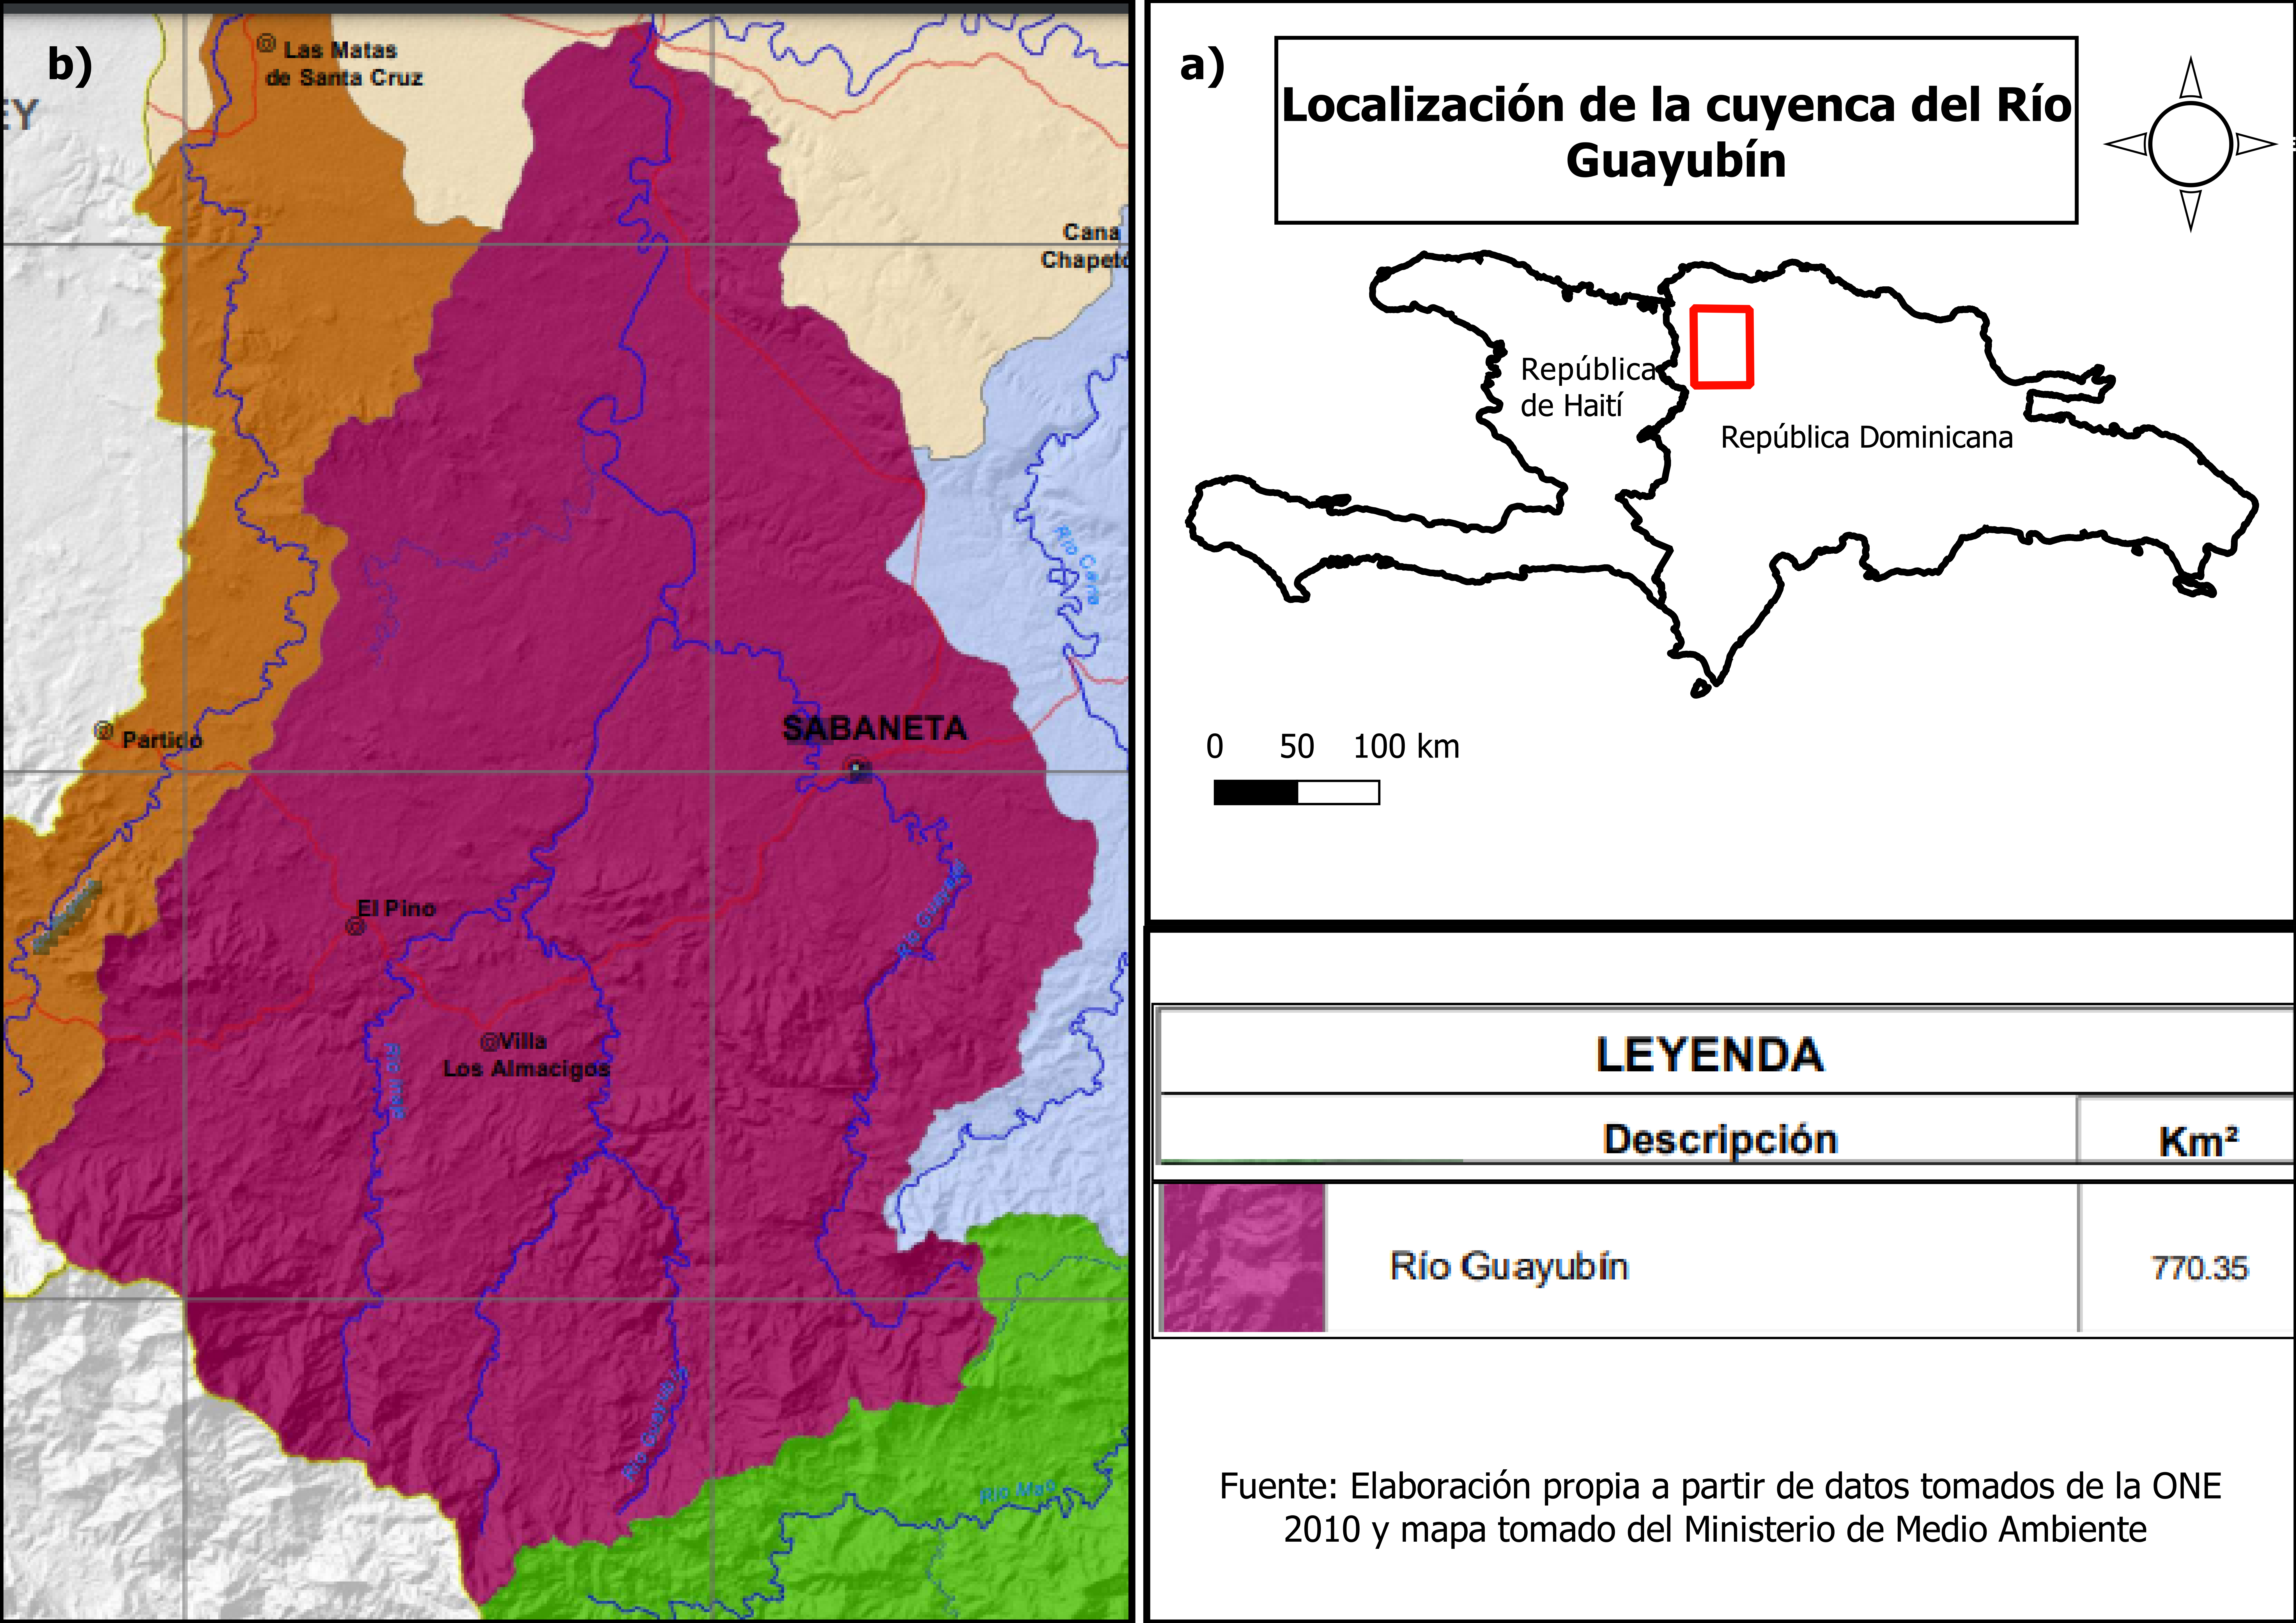
\includegraphics[width=0.90000\textwidth]{Mapa final.png}
\caption{Cuenca del río Guayubín\label{mapacuenca}}
\end{figure}

\section{Materiales y Metodología}\label{materiales-y-metodologuxeda}

Para este estudio se utilizaron operaciones de análisis morfométrico de
redes de drenaje y cuenca de los paquetes de software de código abierto
Grass Gis (Neteler, Beaudette, Cavallini, Lami, \& Cepicky, 2008) por
medio de entorno de programación R (Allaire, 2012). Todos los análisis
de carácter estadísticos y las figuras de los resultados, fueron
realizadas en R usando diversos paquetes (ver tabla
\ref{tab:materiales}). Se utilizó un modelo digital de elevaciones (en
lo adelante, \texttt{MDE}) de la misión radar del transbordador espacial
Shuttle (Farr et al., 2007), a 90 metros de resolución, para extraer los
datos a analizar e interpretar.

Los parámetros de la cuenca acumulación de flujo, elevación, drenaje,
cuenca y otros más, fueron calculados por medio del addon de GRASS GIS
\texttt{r.watershed} (Ehlschlaeger \& Laboratory, 2003--2021b), con un
umbral de acumulación de 80 celdas, utilizando un MDE. Las capas
generadas fueron ingresadas a R con la librería \texttt{sp} y manejadas
con la librería \texttt{raster}.

Para extraer la cuenca se usó el addon \texttt{r.water.outlet}
(Ehlschlaeger \& Laboratory, 2003--2021a), también, se usó el addon
\texttt{r.to.vect} (GRASS Development Team, 2003--2021) para convertir
el ráster resultante en vectorial, que luego se llevó a R. Así mismo, se
aplicó el addon \texttt{r.stream.extract} (Metz, 2003--2021) para poder
extraer la red de drenaje, donde se llevaron a R los resultados
obtenidos.

En cuanto al orden de red y el análisis hortoniano, se usó el addon
\texttt{r.stream.extract} (Metz, 2003--2021) para producir un mapa de
dirección de flujo. Mientras que, para la creación de mapas de ordenes
de red se utilizó el addon \texttt{r.stream.order} (J. Jasiewicz,
2003--2021), donde se usó la clasificación de Strahler para analizar el
orden de red de la cuenca.

También, se usaron los addons \texttt{r.info} (O'Shea \& Laboratory,
2003--2021), para obtener los valores mínimos y máximos del orden de red
según Strahler a partir de un ráster, y, se delimito la cuenca a través
de la red de drenaje con \texttt{r.stream.basins} (J. Jasiewicz,
University, Geoecology, \& Institute, 2003--2021). En cuanto a las
estadísticas según orden de red de Horton para las redes de Strahler y
Horton, se usó el addon \texttt{r.stream.stats} (j. Jasiewicz,
University, \& Geoinformation Institute, 2003--2021) que resume las
estadísticas.

Para calcular los índices de concavidad y los perfiles longitudinales,
primero, se obtuvieron los cursos más largos de la cuenca a través de la
función \texttt{LfpNetwork} (José Ramón Martínez Batlle, 2018b). Y,
luego, se empleó la función \texttt{LfpProfilesConcavity} (José Ramón
Martínez Batlle, 2018c), con la que se obtuvieron los índices de
concavidad para los cursos más largos, y, así mismo, sus perfiles
longitudinales.

Tras crear una nueva región de GRASS en R, se convirtieron a números
enteros la extensión y la resolución del DEM con las funciones
\texttt{integerextent} (José Ramón Martínez Batlle, 2020a), y
\texttt{xyvector} (José Ramón Martínez Batlle, 2018d). También, se usó
la herramienta \texttt{gdalwarp} (Warmerdam, Rouault, \& others,
1998--2021), para reproyectar y deformar ráster. Se utilizaron los
addons \texttt{g.proj} (Kelly, 2003--2021), y \texttt{r.in.gdal}
(Warmerdam, 2003--2021), para importar a la sesión de GRASS. Se usó el
addon \texttt{r.stream.extract} (Metz, 2003--2021) para generar una red
de drenaje y obtener coordenadas que serían transformadas a EPSG: 4326
(Lohmar, 1988), como número entero con la función \texttt{My\_Trans}
(José Ramón Martínez Batlle, 2020b).

En cuanto a la obtención de los parámetros morfométricos de la cuenca se
usa el addon \texttt{r.basin} (Di Leo \& Di Stefano, 2003--2021). Los
vectores obtenidos son transformados a EPGS: 4326 (Lohmar, 1988), y así
visualizados con la librería \texttt{leaflet}. También, para explorar
los parámetros de la cuenca se usó la librería \texttt{readr}.

Finalmente, para el cálculo de la curva y la integral hipsométrica, lo
primero fue representar las cuencas con las librerías \texttt{sp} y
\texttt{mapview}; y segundo, calcular la integral y curva hipsométrica
utilizando la función \texttt{HypsoIntCurve} (José Ramón Martínez
Batlle, 2018a).

\section{Resultados}\label{resultados}

El fruto del estudio realizado a la cuenca del río Guayubín usando el
\texttt{script\ reproducible}, produce información que facilita el
análisis y comprensión de la cuenca fluvial, tanto de manera agrupada,
como de forma desagregada. A continuación, se presentan de manera
resumida, las características morfológicas principales de la cuenca y su
red de drenaje.

La cuenca del río Guayubín muestra una área de 773.56
km\textsuperscript{2} y un perímetro de 156.12 km, siendo la tercera más
grande de la cuenca del Yaque del Norte por su extensión; la misma
alcanza una elevación, aproximada, máxima de 1396.73 m, media de 276.70
m y una mínima de 30.97 m, por lo que se puede decir que su relieve es
muy heterogéneo (ver tablas \ref{tab:estadisticaor} y
\ref{tab:parametrosm}).

Al observarse la figura \ref{forma} la forma de la cuenca es alargada de
sur a norte, además, es ancha, siendo la parte sur más ancha que la
norte de la misma, dando lugar a una cuenca en forma de pera. En ese
mismo contexto, los parámetros de coeficiente de compacidad, forma de la
cuenca y razón de elongación, confirman, de igual manera, que la cuenca
es alargada y ancha (ver tabla \ref{tab:parametrosm}). En cuanto a la
red de drenaje de la cuenca, se presentan patrones de drenaje
dendríticos, siendo bastante densa con ramificaciones muy regulares
principalmente en la cuenca alta, al sur (ver figura
\ref{red de drenaje extraida}); esto se debe a que el relieve es
medianamente accidentado, y a que la composición o material rocoso
existente como la arenisca, rocas calcáreas, limolita, conglomerado y
otros (ver figura \ref{geologico}).

La red de drenaje de la cuenca, según Strahler, presenta un total de 367
redes (ver tabla \ref{tab:estadisticaor}) y se organiza por órdenes de
red desde orden uno hasta orden cinco (ver figura \ref{unica}, y figura
\ref{subcuencas}). Donde las redes de drenaje de orden uno suman un
total de 284, siendo los primeros, tributarios de la red y poseen una
longitud corta, pues depositan sus aguas y alimentando a otro curso de
agua que pasaría a tener una jerarquía mayor (repitiéndose el proceso
hasta llegar al curso principal); las redes de orden 2 que se producidas
fueron un total de 61, en este clasificación se ve una reducción en el
número de redes, presentando un aumento en el orden y un descenso en las
redes de drenaje que lo integran; para el orden 3 un total de 17 redes
de drenaje; para el orden 4 se produjeron 4 redes; y para el orden 5 se
produjo una sola red, siendo este el principal curso de agua de toda la
cuenca, que recibe las aguas de las redes de drenaje anteriores (ver
figura \ref{grafnumero}, y tabla \ref{tab:parh}).

En la red de drenaje se percibe la presencia de un fenómeno de
reorganización denominado captura fluvial, presentándose en las redes de
orden 1 que drenan en redes de orden 2, 3, 4 e incluso en la de orden 5,
esto se produce para cada orden que deposita sus aguas en otro curso
(ver figuras \ref{unica}, \ref{grosor} y figura \ref{subcuencas}).

Con la función \texttt{LfpNetwork} se obtuvieron los cursos más largos
de la red de drenaje, siendo un total de 60 cursos, de los cuales se
generaron los perfiles longitudinales y se obtuvieron los índices de
concavidad. Los perfiles de estos cursos mostraron ser positivos para la
gran mayoría de estos; otros cursos presentan índices negativos de
concavidad (son convexos); y una minoría son rectilíneos (ver figuras
\ref{lfpnet} y \ref{plongitudinal}).

De los cursos más largos, el que más destaca es el curso número 1 o
Gyb-1 (ver figuras \ref{plongitudinal} y \ref{indicec}), con un índice
de concavidad de 0.6, y que también encaja con el curso de nombre
\texttt{río\ Guayubín} en el mapa topográfico de República Dominicana
(Lizmap, s.f.), más la cabecera de este curso coincide con el del arroyo
\texttt{La\ Yaya}, que drena sus aguas en el río \texttt{Yaguajal}. El
curso tiene una dirección general de sur a norte; presentando dos
sobresaliente convexas muy destacadas, la primera se produce donde hay
un cambio en su dirección donde entran en contacto el conglomerado:
molasa continental con rocas magmáticas y volcano-sedimentarias,
normalmente originadas en arcos de islas, tomando dirección
suroeste-noreste; y la segunda se genera, donde entran en contacto el
conglomerado: molasa continental con limolita calcárea, arenisca,
conglomerado y caliza detrítica, produciéndose, nuevamente, un cambio de
dirección sudeste-noroeste (Mollat, Wagner, Cepek, \& Weiss, 2004). Otro
curso de agua que destaca por su alto índice de concavidad (0.56), es el
número 37 o Gyb-37 (ver figuras \ref{plongitudinal} y \ref{indicec}), el
cual corresponde al río Aminilla del mapa topográfico de República
Dominicana (Lizmap, s.f.). Este curso tiene una dirección
suroeste-noreste.

Mientras que los cursos de agua más largos con índices de concavidad
negativo, que más destacan son el 18 o Gyb-18, con -0.13, siendo este
convexo. Este coincide con el curso Cañada Prieta del mapa topográfico
de República Dominicana (Lizmap, s.f.), la cual tiene una dirección
sur-norte, presentando pequeños pliegues en su trayecto, no relacionados
a la litología, puesto que, corre sobre limolita calcárea, arenisca,
conglomerado y caliza detrítica, lo que resulta irregular. Lo mismo
ocurre en los cursos 25, 32, que corresponden a Arroyo seco y arroyo El
Mamey en el mapa topográfico del país (Lizmap, s.f.), su convexidad no
está relacionada con la litología (ver figuras \ref{plongitudinal},
\ref{indicec} y \ref{geologico}).

A diferencia de los cursos convexos que no se destacan cambios en su
litología (18, 25 y 32), el curso de agua 59 o Gyb-59, con un índice de
concavidad de -0.14, es un pequeño arroyo o cañada sin nombre que
desagua en el río Yaguajal (Lizmap, s.f.). Realiza más de la mitad de su
recorrido por tonalita y luego por rocas magmáticas y
volcano-sedimentarias; de sus pequeños pliegues se destaca el que se
produce en la zona donde entran en contacto las rocas mencionadas
anteriormente, por lo que su convexidad en tal punto puede estar
relacionada a la litología (ver figuras \ref{plongitudinal},
\ref{indicec} y \ref{geologico}).

También, están los cursos que son casi rectilíneos, como el curso 28 o
Gyb-28, con un índice de concavidad de 0.18 (bastante bajo), es
rectilíneo en un 50\%, en su parte central. Este coincide con el arroyo
Canario (Lizmap, s.f.), y realiza el 90\% de su recorrido por limolita
calcárea, arenisca, conglomerado y caliza detrítica, mientras su
desembocadura en el río Guayubín asentado sobre rocas metamórficas
regionales: facies esquito verde. Aunque su morfología no se debe al
cambio en su litología (ver figuras \ref{lfpnet}, \ref{plongitudinal} y
\ref{indicec}).

Según los parámetros morfométricos de la cuenca el curso más largo de
toda la cuenca no coincide con el obtenido con la función
\texttt{LfpNetwork} (curso 1), sino, que coincide con el curso 30
obtenido por la función; Este curso coincide con el arroyo Dajao que
está en el mapa topográfico del país (Lizmap, s.f.); este posee una
longitud de 61.96 km (ver figura \ref{vectoresrbasin}).

De los parámetros de la cuenca que guardan una relación con la
litología, la densidad de drenaje es uno de ellos, el cual para la
cuenca fue 0.85 km/km\textsuperscript{2}. También, está la de razón de
Bifurcación (3.8) para toda la cuenca, considerando que el relieve de la
cuenca es accidentado y que gran parte de la misma está en la montaña
(ver figura \ref{tab:parametrosm}). En ese mismo contexto, la razón de
bifurcación se mantuvo constante para las redes de drenaje de orden 1, 3
y 4, aunque, la red de orden 2 no difiere por mucho de la razón de
bifurcación de la cuenca (ver figura \ref{tab:razones}).

Las estadísticas que se generaron sobre la curva y la integral
hipsométrica se obtuvieron 60 resultados para los cursos de agua
pertenecientes a la cuenca de orden 2. Donde los cursos más curvos
fueron 37 y 18; el primero presenta signos de una evolución lenta en su
elevación; y el segundo, presenta una evolución media en su elevación. Y
los cursos 41 y 42 son los más rectilíneo y su integral hipsométrica es
moderada por lo que estos cursos han experimentado una evolución lenta
en su elevación (ver tabla \ref{tab:ihco2} y figuras \ref{hypsob2} y
\ref{hypb2}).

En cuanto a los cursos de agua de las cuencas de orden 3, se produjeron
17 resultados. Donde los cursos con los valores máximos presentes (8 y
13), tuvieron una evolución media en la elevación. Y los cursos 4 y 16,
demuestran una lenta y estable evolución en la elevación (ver tabla
\ref{tab:ihco3} y figuras \ref{hysob3} y \ref{hypb3}).

\section{Discusión}\label{discusiuxf3n}

Con los hallazgos producidos sobre la cuenca del rio Guayubín, se
responden las preguntas planteadas sobre la forma de la cuenca y su red
de drenaje, la organización de la red de drenaje, la relación de los
perfiles longitudinales y su índice de concavidad con la litología en la
cuenca. En cambio, las preguntas sobre la relación de los parámetros de
cuenca con la litología, al igual que la relación de la curva
hipsométrica y la integral con la litología, no fueron respondidas del
todo, por lo que necesitan un análisis más detallado. Estos hallazgos se
corresponden con algunas informaciones que se conocen de la cuenca, como
su área, que difiere, por muy poco, de los que se conocen de Medio
Ambiente y Recurso Naturales (2015).

En los parámetros de cuenca y en las estadísticas de ordenes de red, el
valor de área de cuenca se mantuvo sin cambios; pero comparándolos con
las informaciones extraídas de Medio Ambiente y Recurso Naturales
(2015), los valores que se obtuvieron no concuerdan, puesto que, la
cuenca presentada por Medio Ambiente y Recurso Naturales (2015), es más
pequeña que la producida por los algoritmos en R; aunque la diferencia
es muy poca (ver tablas \ref{tab:parametrosm} y
\ref{tab:estadisticaor}).

La cuenca tiene forma de pera (Terrain Works Team, 2014), y la forma de
su red de drenaje es dendrítica (Gutiérrez Elorza, 2008). La forma de la
red de drenaje se produce en zonas de relieve heterogéneo como se
presenta la parte de cuenca alta; los cursos de agua se desarrollan
libremente y no depende de un control estructurales (Ingeniero Civil
Team, 2018). Howard (1967), asegura que en los patrones dendríticos los
sedimentos tienen una resistencia uniforme.

La red de drenaje de la cuenca presenta signos de haber sufrido el
fenómeno de reorganización captura fluvial, según Pastor (2013) este
fenómeno se puede identificar al observar la red de drenaje, donde se
producen cambios abruptos en el recorrido del cauce que ha sido captura.
Se ha observado que este fenómeno se produce en todas las redes desde
orden 1 a orden 5, en especial en las redes de orden más bajo, pero
puede verse muy marcado en la red de orden cinco, donde se produce
cambios del tipo de roca y relieve es más heterogéneo (ver figura
\ref{grosor} y \ref{geologico}).

Según Summerfield (1991), la razón de bifurcación que esta entre 3 y 5,
indica que la litología del lugar es homogénea. En tabla
\ref{tab:razones}, es visible como los valores para la razón de
bifurcación en los órdenes de red difieren el uno del otro, los órdenes
1, 2, 3 y 4 mantienen una homogeneidad en su litología. Como se observa
en las tablas \ref{tab:regresionc} y \ref{tab:estandard}, las razones de
bifurcación obtenidas se corresponden. Ambos valores coinciden con la
razón de bifurcación calculada con código en R (4.064346), podemos
concluir que mantienen una constancia en el tipo de roca presente.

Los cursos más largos de la red de drenaje que tienen los más altos
índices de concavidad fueron los cursos 30, 48, 52, 55 y 56; estos
sufrieron de cambios en su trayecto y están relacionados con la
aparición de una roca dura, tras haber comparado los resultados de los
cursos más largo en el mapa geológico nacional (Mollat et al., 2004), se
comprueba que existe un cambio en la litología presente en los cursos de
agua, en el caso del curso 30 (con un índice de 0.59 de concavidad), al
pasar de estar sobre rocas tonalitas a estar sobre rocas sedimentarias y
de originadas en arcos de islas se produce un cambio en su trayectoria.

También se vio afectado el curso de agua 19, quien presenta un índice de
concavidad de 0.46 producto de que este flujo en su trayecto se
encuentra con una falla tectónica, provocando el cambio en su curso. Y
los cursos más rectilíneos con los índices de concavidad más bajos son
los cursos de agua número 15, 16, 23 y 38; estos cursos de agua realizan
su recorrido por un mismo tipo de roca por lo que no experimenta cambios
bruscos en su curso (ver figura \ref{lfpnet}, \ref{plongitudinal} y
\ref{indicec}).

Los parámetros morfométricos obtenidos (ver tabla
\ref{tab:parametrosm}), como el coeficiente de compacidad que indica que
la forma de la superficie de la cuenca de acuerdo con su delimitación, y
el predominio en su escorrentía, es muy alargada (López Cadenas de Llano
\& Mintegui Aguirre, 1986); pero, el parámetro forma de la cuenca generó
un índice que indica que la cuenca además de ser muy alargada está
bastante ensanchada en las zonas de cuenca alta y cuenca media (Córdova,
2016; Pérez, 1979). Según los resultados de la razón de elongación, se
confirma que la cuenca es alargada (De Matauco, 2004).

El curso más largo de la red de drenaje o curso principal en la cuenca,
producido por \texttt{r.basin} tiene una longitud 61.96 km; según una
comparación realizada entre el vectorial de cursos más largo (ver figura
\ref{lfpnet}), y el curso que se obtuvo con \texttt{r.basin} (ver figura
\ref{vectoresrbasin}), es el curso numero 30 obtenido con la función
\texttt{LfpNetwork}. Por lo que la cabecera del rio Guayubín se localiza
al sureste de la indicada por Medio Ambiente y Recurso Naturales (2015),
bajo el nombre de Dajao.

La curva y la integral hipsométrica muestran la repartición de
elevaciones en la cuenca (Jose Ramon Martinez Batlle, 2019). El valor
mínimo generado para la integral hipsométrica fue 0.08 en el curso 43.
En tanto, el valor máximo para la integral fue de 0.48 en el curso 45
(ver tabla \ref{tab:ihco2}). Y los cursos más curvos fueron 37 y 18. El
primero presenta signos de una evolución lenta en su elevación; y el
segundo, presenta una evolución media en su elevación. Ver figuras
\ref{hypsob2} y \ref{hypb2}. Los cursos 41 y 42 son los más rectilíneo y
su integral hipsométrica es moderada por lo que estos cursos han
experimentado una evolución lenta en su elevación.

Los cursos de agua pertenecientes a la cuenca de orden 3, los valores
máximos presentes (8 y 13), tuvieron una evolución media en la
elevación. Y los cursos 4 y 16, demuestran una lenta y estable evolución
en la elevación (ver tabla \ref{tab:ihco3} y figuras \ref{hysob3} y
\ref{hypb3}).

Toda la información generada sobre la cuenca sirve como peldaño a
futuras investigaciones sobre la misma u otras cuencas fluviales en el
país.

El estudio está limitado a los análisis cuantitativos, puesto que carece
de la toma de muestras en campo para una más precisa comprensión de la
cuenca.

\section{Agradecimientos}\label{agradecimientos}

A Dios por la fuerza y la salud que me ha otorgado todo este tiempo, sin
dejarme caer.

A mi maestro \texttt{Jose\ Martínez\ Batlle} por el apoyo incondicional,
tanto emocional como técnico, por ser guía durante todo el trayecto, por
ser paciente, y sobre todo por su disponibilidad para colaborar.

A mi compañero de carrera y amigo \texttt{Welifer\ Lebron} por su
asesoramiento.

A mis compañeros
\texttt{Saderis\ Carmona,\ Franklin\ Gomez,\ Randy\ Mueses,\ Frank\ de\ la\ Cruz\ y\ Cinthia\ Vandepool}
con los que me embarqué en este nuevo reto, tres meses atrás, y de los
cuales recibí apoyo emocional y técnico.

A mi madre \texttt{Denny\ Laureano}, mis hermanos
\texttt{Darleny\ Linares,\ Diana\ Carolina\ Linares\ y\ Jose\ Daniel\ Linares}
por la comprensión y el apoyo tanto moral como emocional durante este
tiempo.

A mis amistades por el apoyo, comprensión y motivación para que continúe
y finalice mis proyectos.

\section{Información de soporte}\label{informaciuxf3n-de-soporte}

\begin{figure}
\centering
\includegraphics[width=0.80000\textwidth]{geologico.png}
\caption{Mapa Geológico de la cuenca\label{geologico}}
\end{figure}

\begin{figure}
\centering
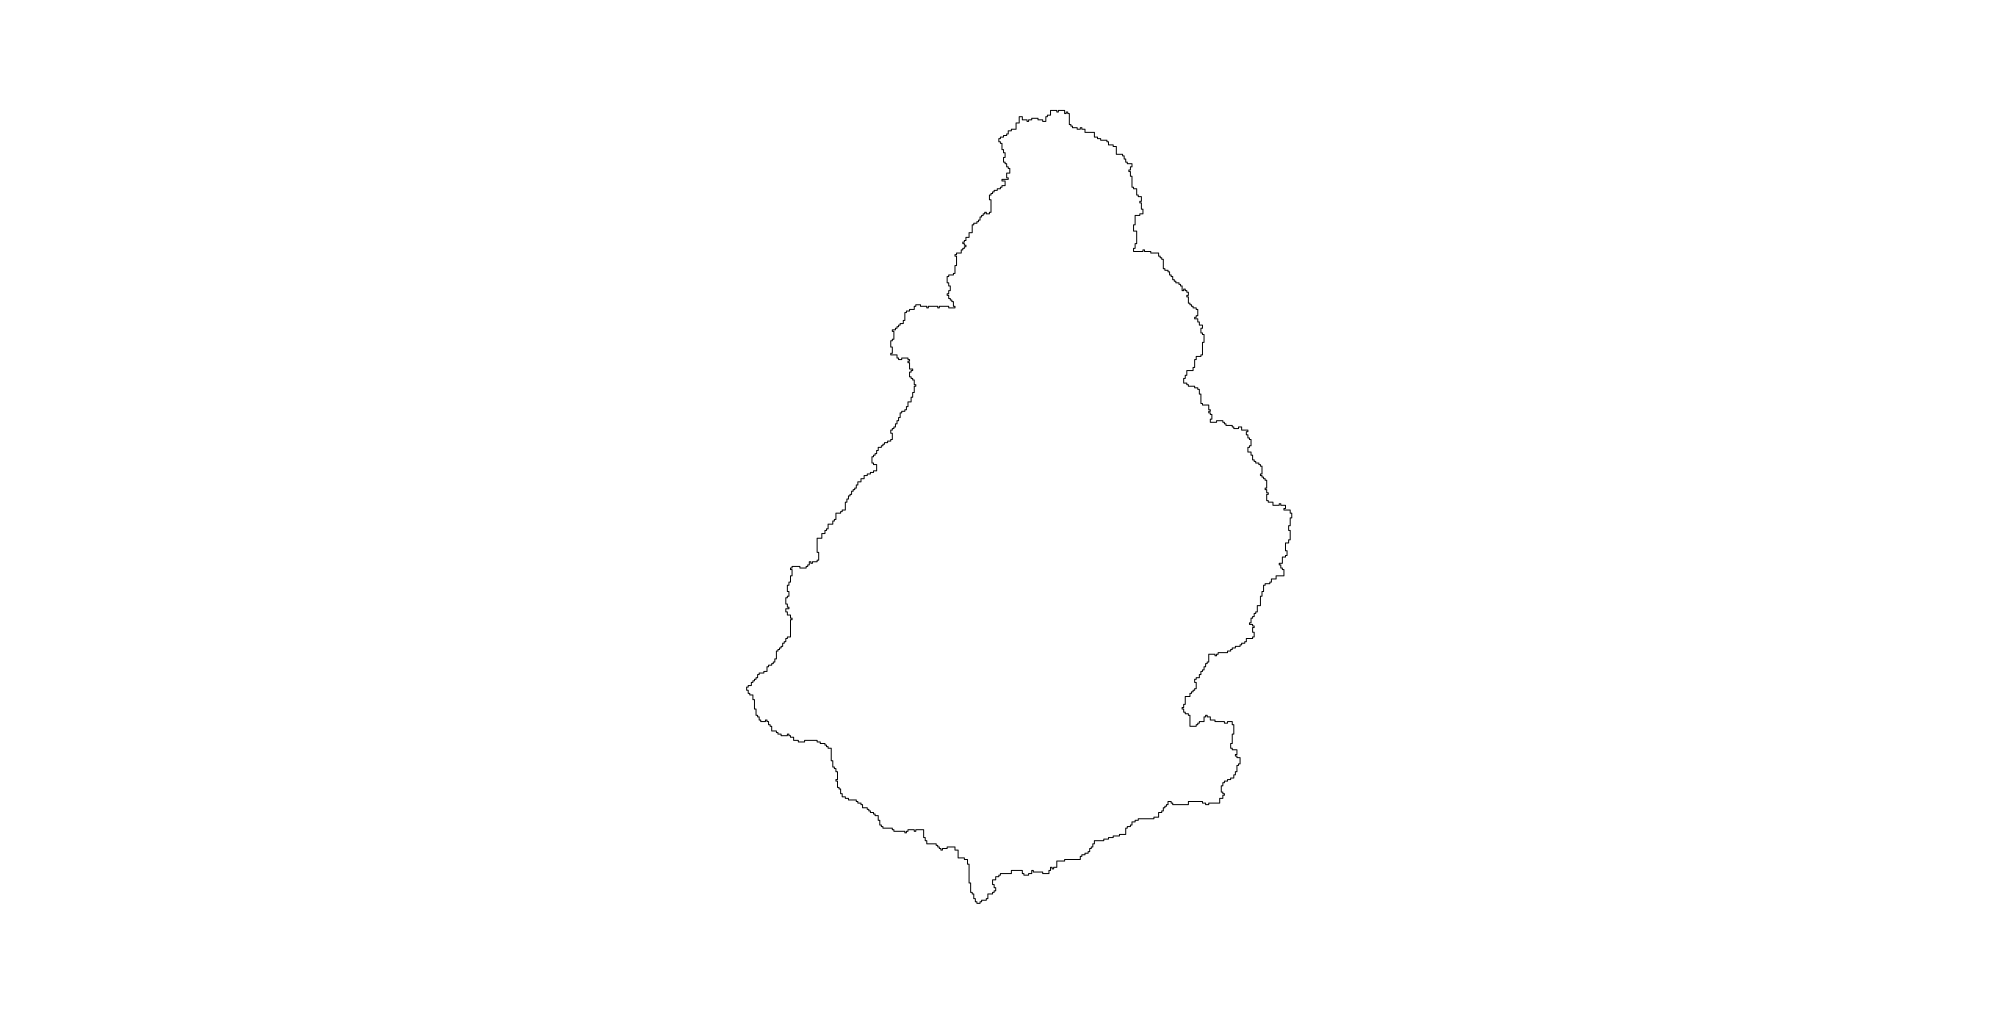
\includegraphics[width=0.50000\textwidth]{cuenca extraida.png}
\caption{Forma de la cuenca del río Guayubín\label{forma}}
\end{figure}

\begin{figure}
\centering
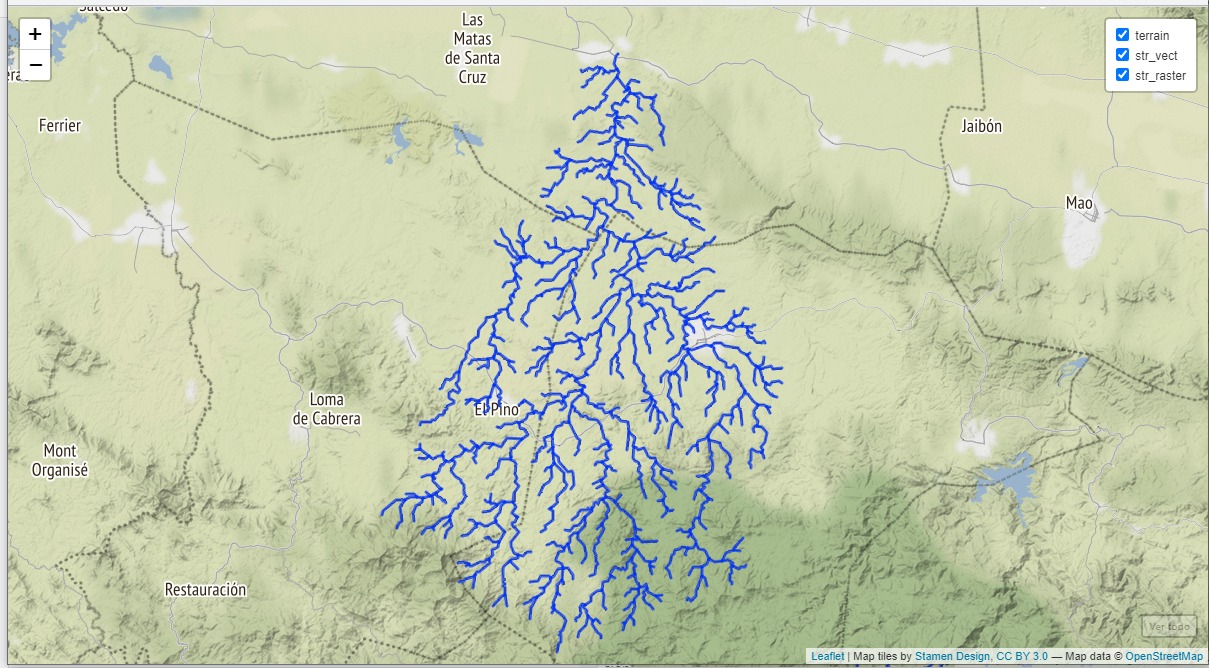
\includegraphics[width=0.70000\textwidth]{red de drenaje extraida.png}
\caption{Red de drenaje del río Guayubín\label{red de drenaje extraida}}
\end{figure}

\begin{figure}
\centering
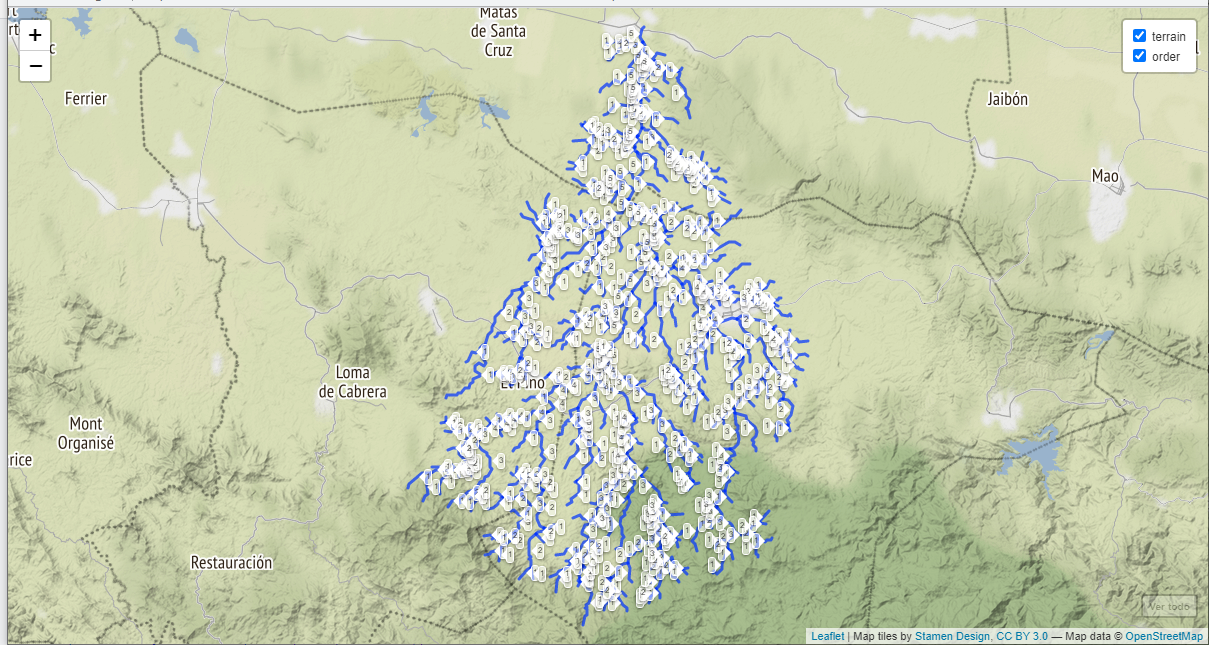
\includegraphics[width=1.00000\textwidth]{ordenes de red.png}
\caption{Ordenes de red del río Guayubín con simbología
única\label{unica}}
\end{figure}

\begin{figure}
\centering
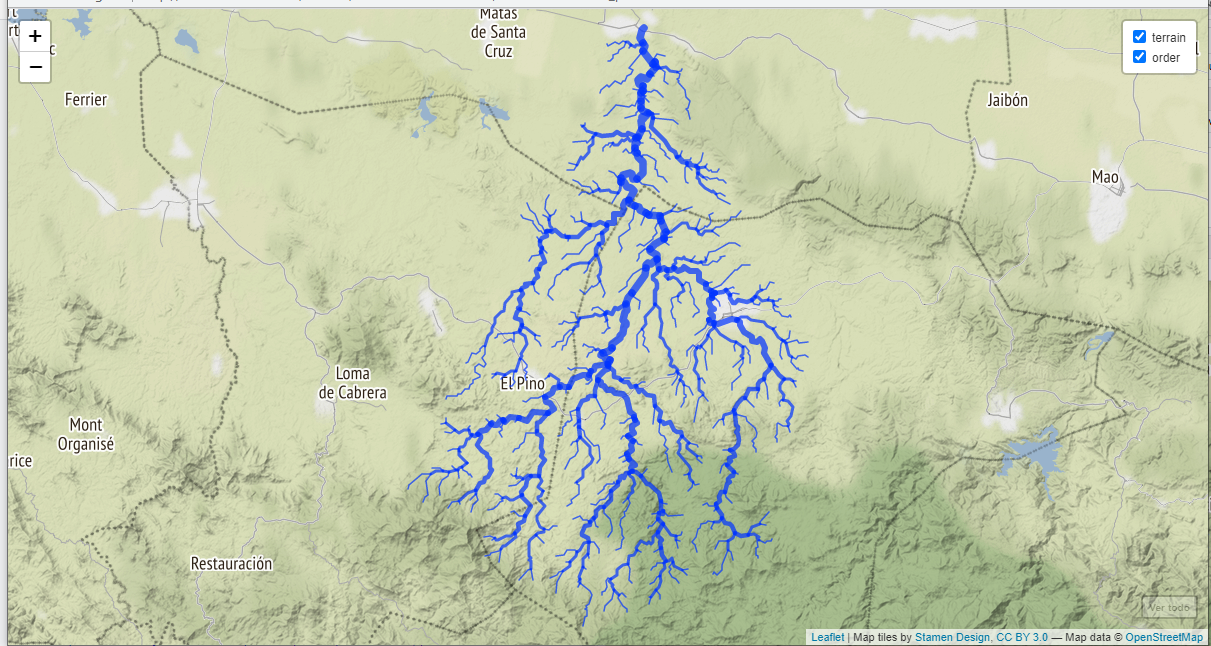
\includegraphics[width=0.80000\textwidth]{orden de red mapa 2.png}
\caption{Ordenes de red del río Guayubín con simbología aplicando grosor
según su orden\label{grosor}}
\end{figure}

\begin{figure}
\centering
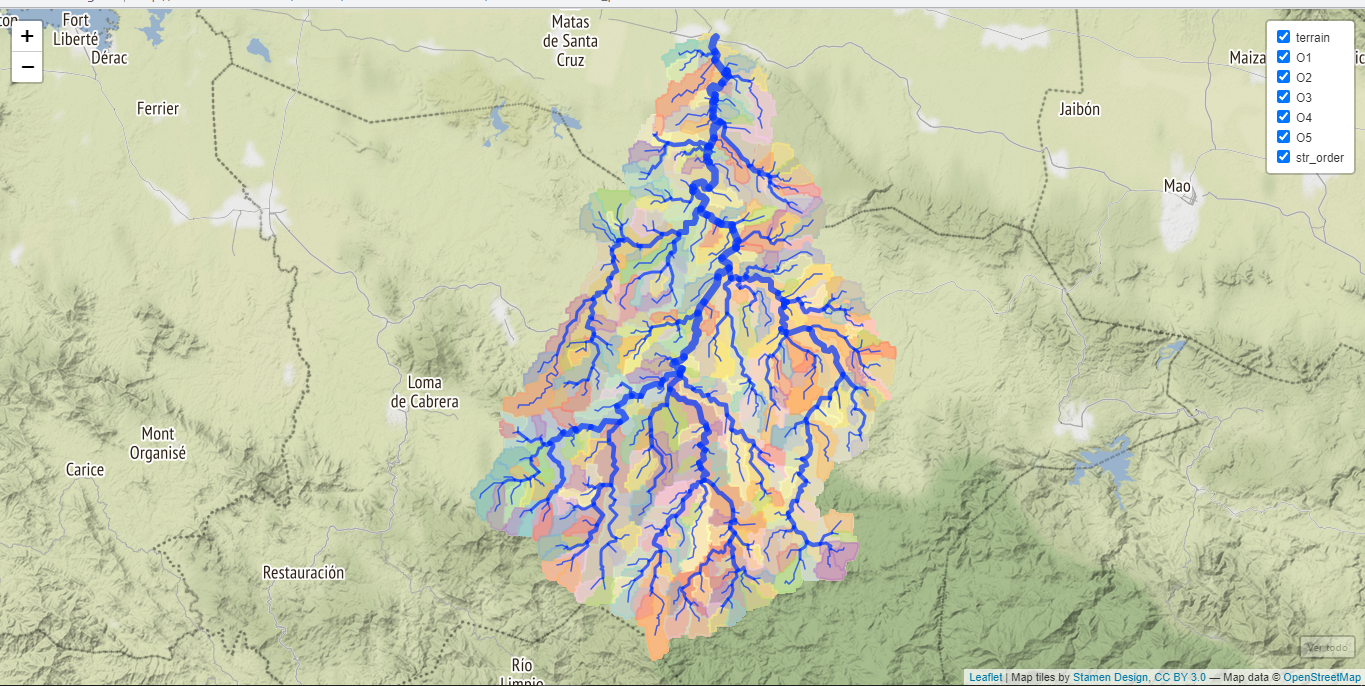
\includegraphics[width=0.70000\textwidth]{cuencas delimitadas y ordenes de red.png}
\caption{Red de drenaje según su orden de red del río
Guayubín\label{subcuencas}}
\end{figure}

\begin{figure}
\centering
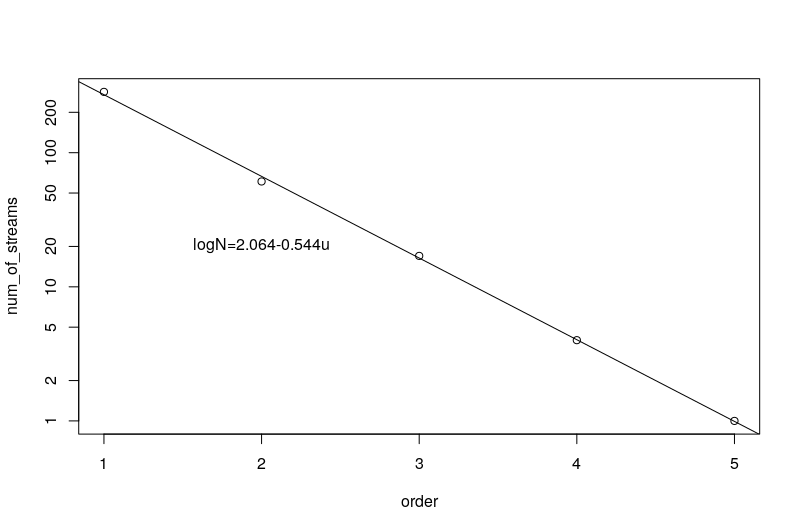
\includegraphics[width=0.80000\textwidth]{Numero de red segun su orden.png}
\caption{Número de redes según su orden y Razón de
bifurcación\label{grafnumero}}
\end{figure}

\begin{figure}
\centering
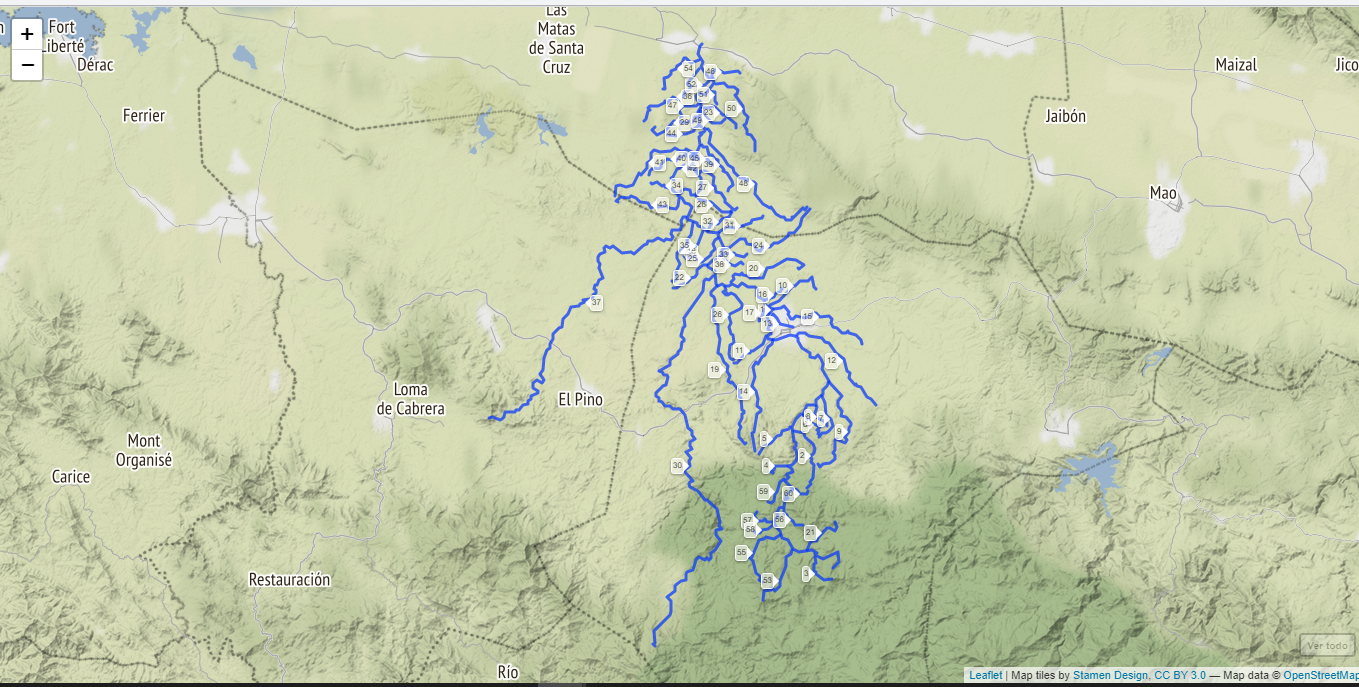
\includegraphics[width=1.00000\textwidth]{cursos mas largos.png}
\caption{Cursos fluviales más largos de la cuenca del río
Guayubín\label{lfpnet}}
\end{figure}

\begin{figure}
\centering
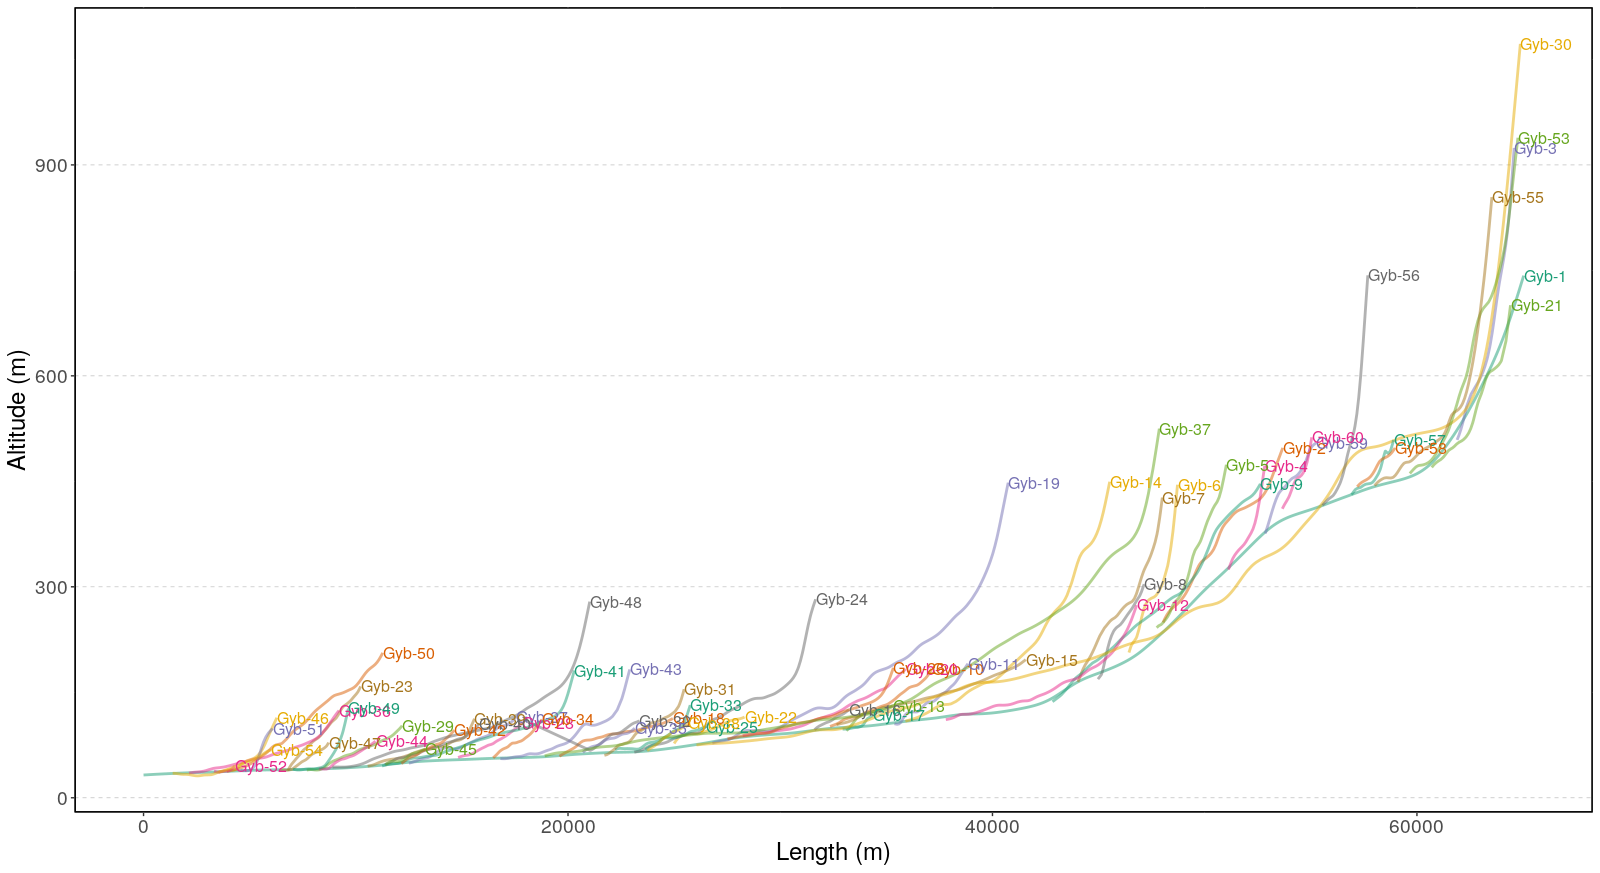
\includegraphics[width=1.00000\textwidth]{perfiles longitudinales.png}
\caption{Perfiles longitudinales de los cursos más largos en la cuenca
del río Guayubín\label{plongitudinal}}
\end{figure}

\begin{figure}
\centering
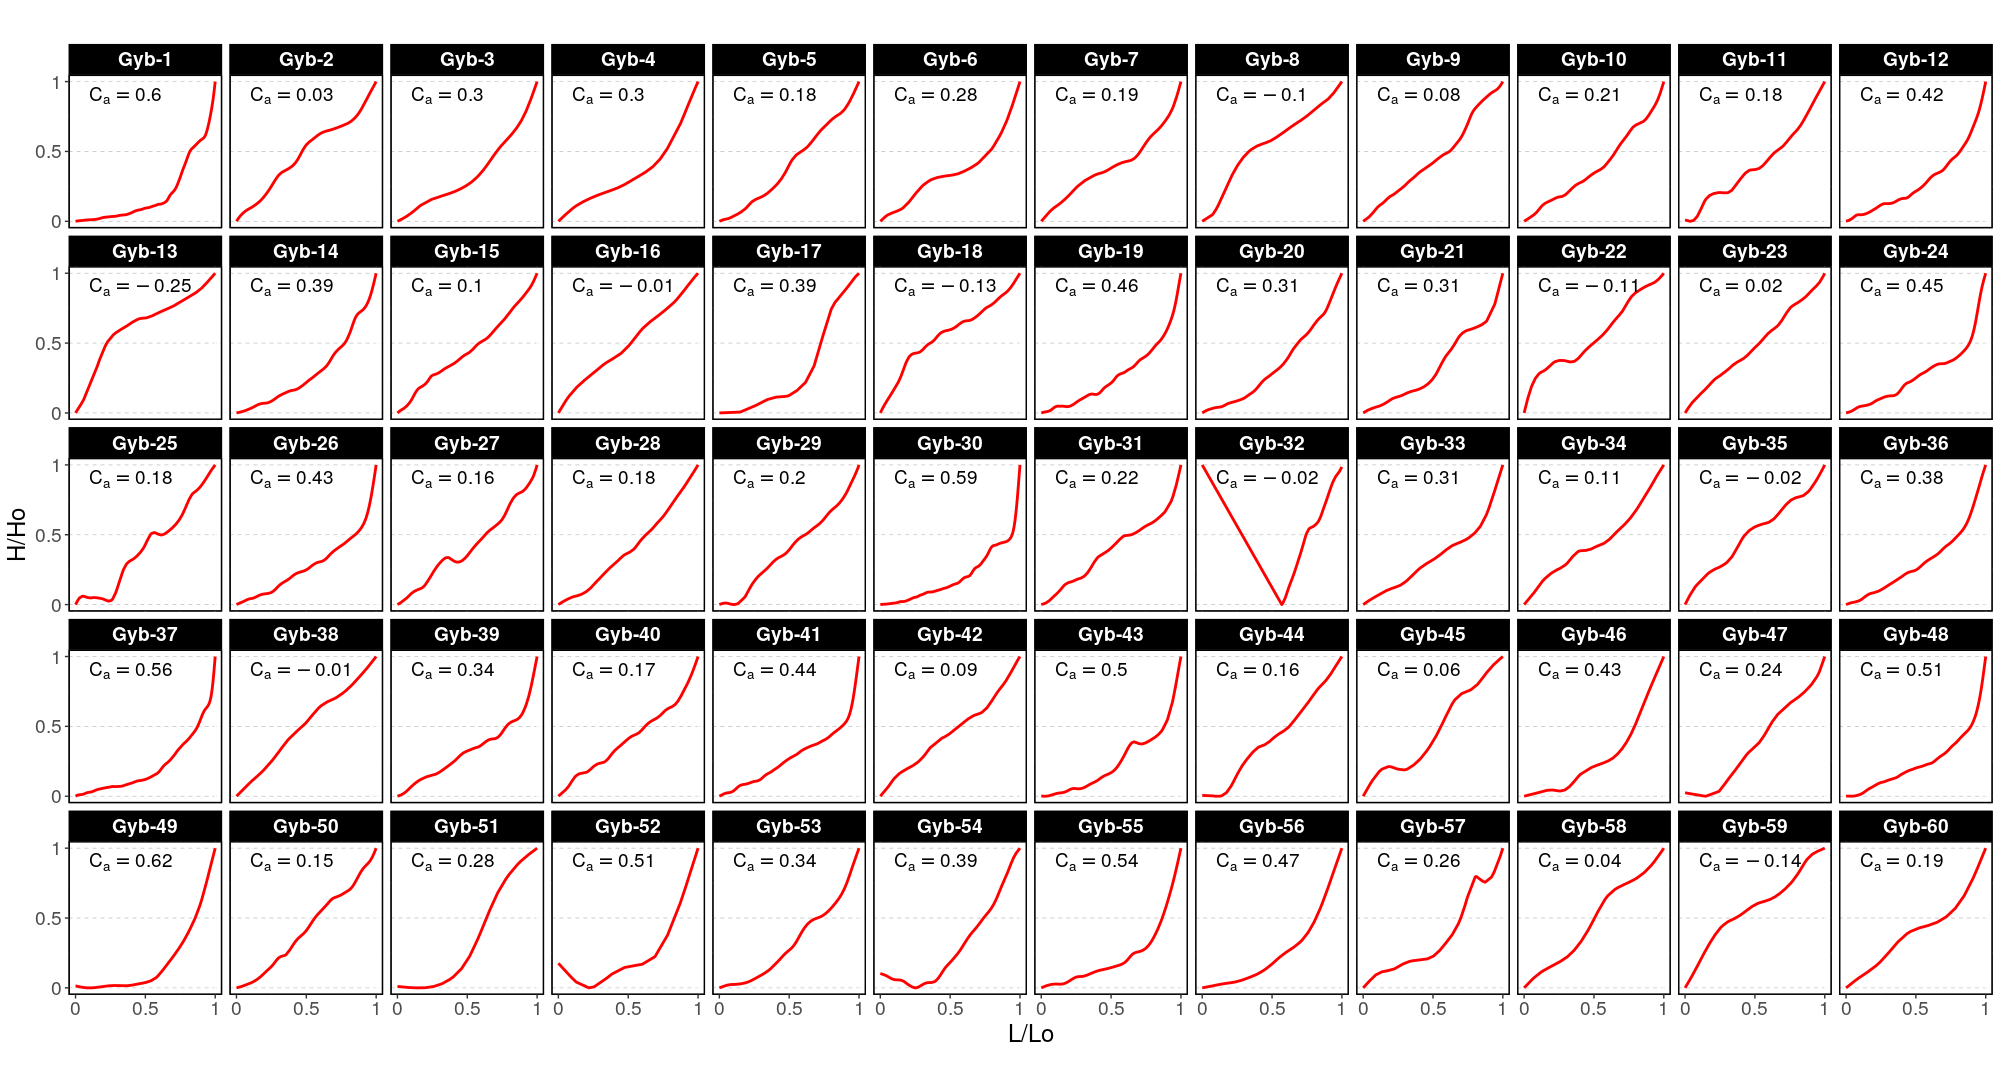
\includegraphics[width=1.00000\textwidth]{Indices de concavidad.png}
\caption{Perfiles longitudinales e índices de concavidad de los cursos
más largos en la cuenca del río Guayubín\label{indicec}}
\end{figure}

\begin{figure}
\centering
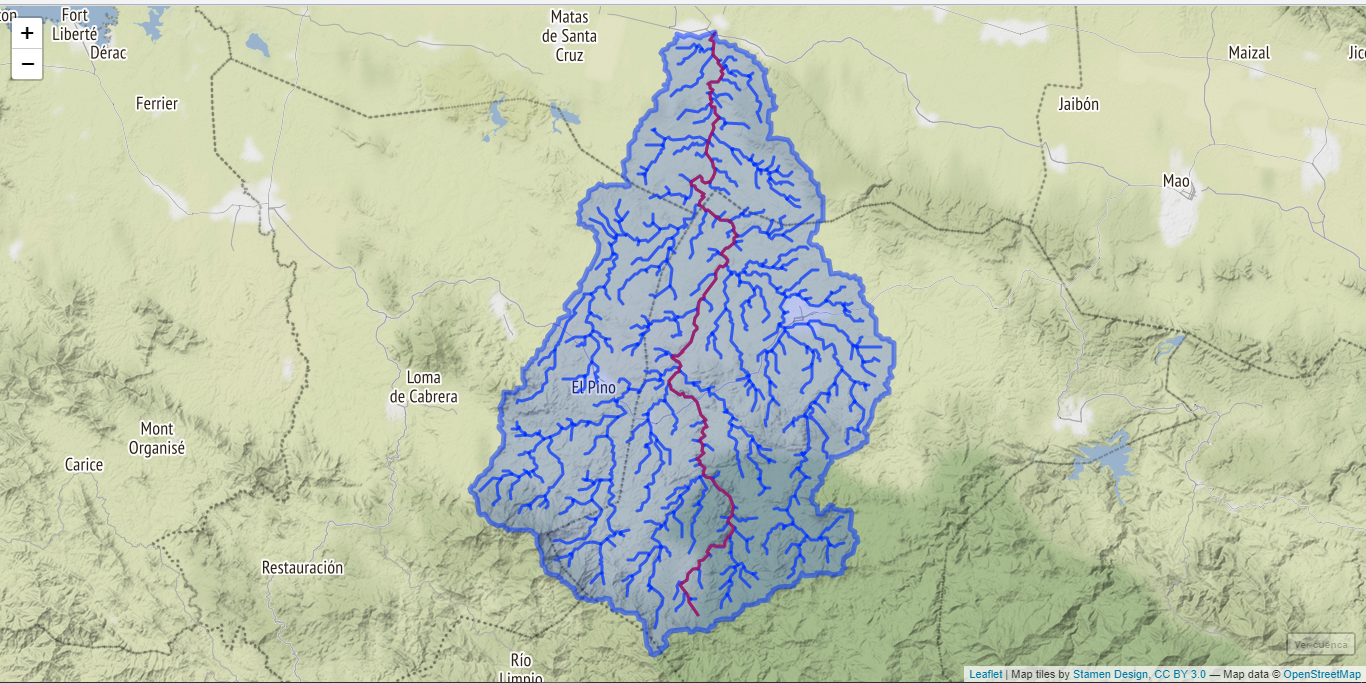
\includegraphics[width=0.60000\textwidth]{cuenca-red de drenaje-curso mas largo.png}
\caption{Cuenca del río Guayubín con su red de drenaje y su curso más
largo\label{vectoresrbasin}}
\end{figure}

\begin{figure}
\centering
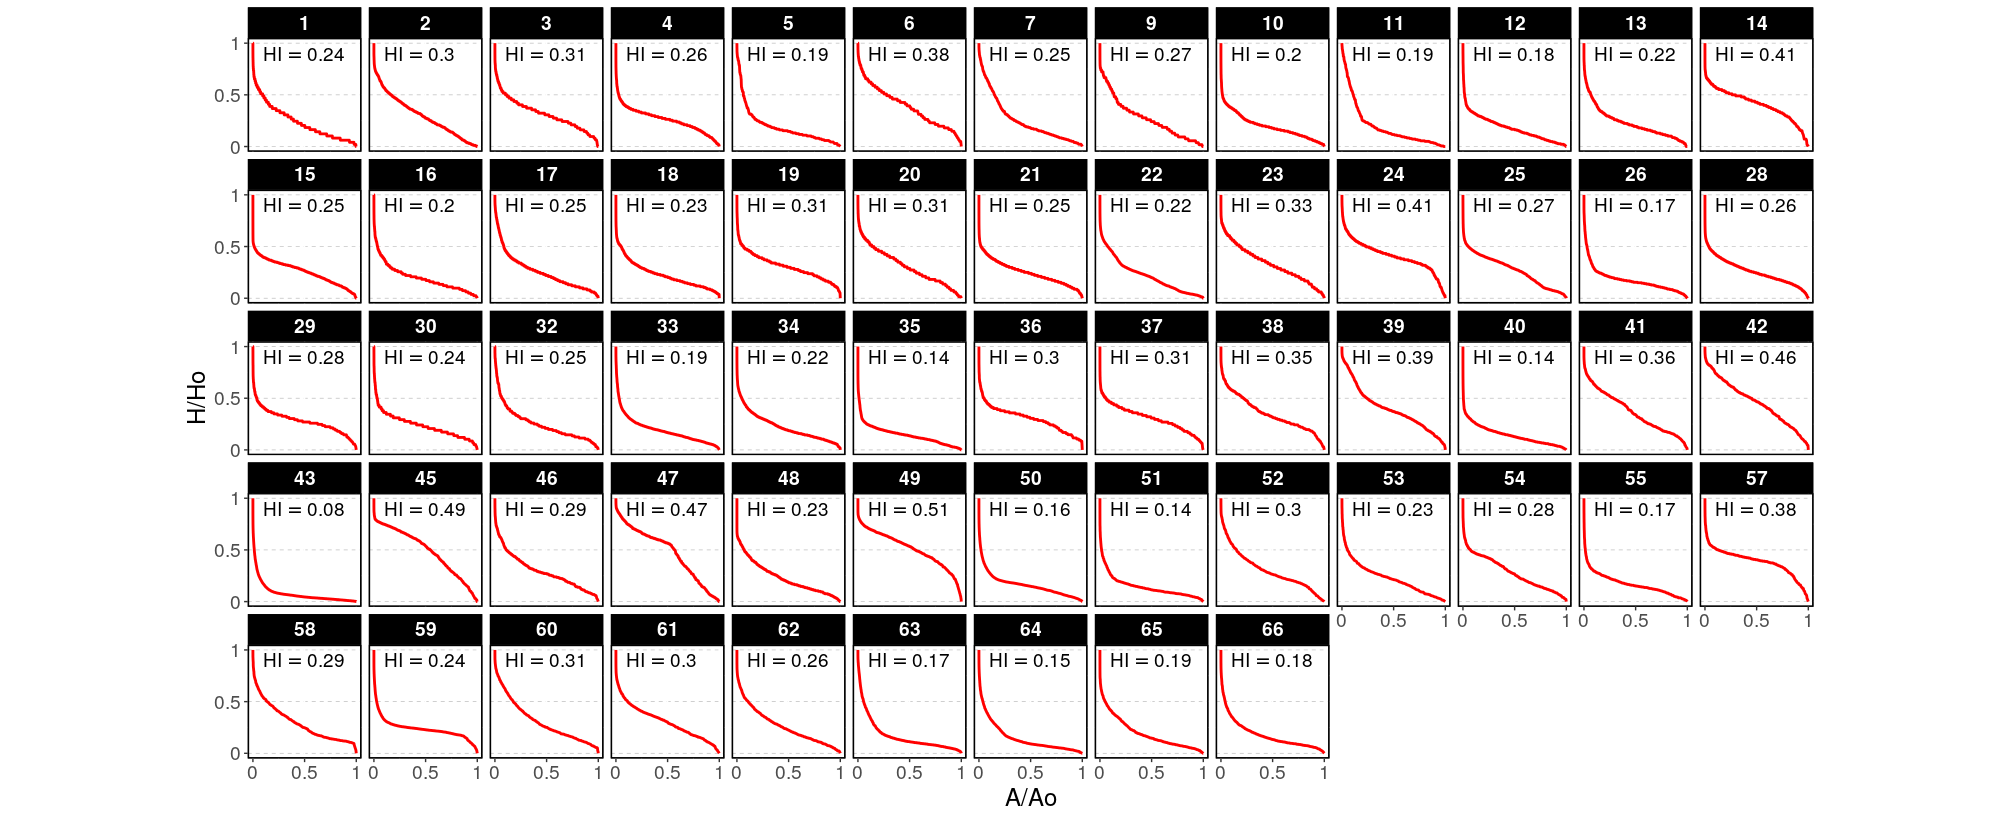
\includegraphics[width=1.10000\textwidth]{HypsoBasinOrder2.png}
\caption{Curva e integral hipsométrica para las cuencas de orden
2\label{hypsob2}}
\end{figure}

\begin{figure}
\centering
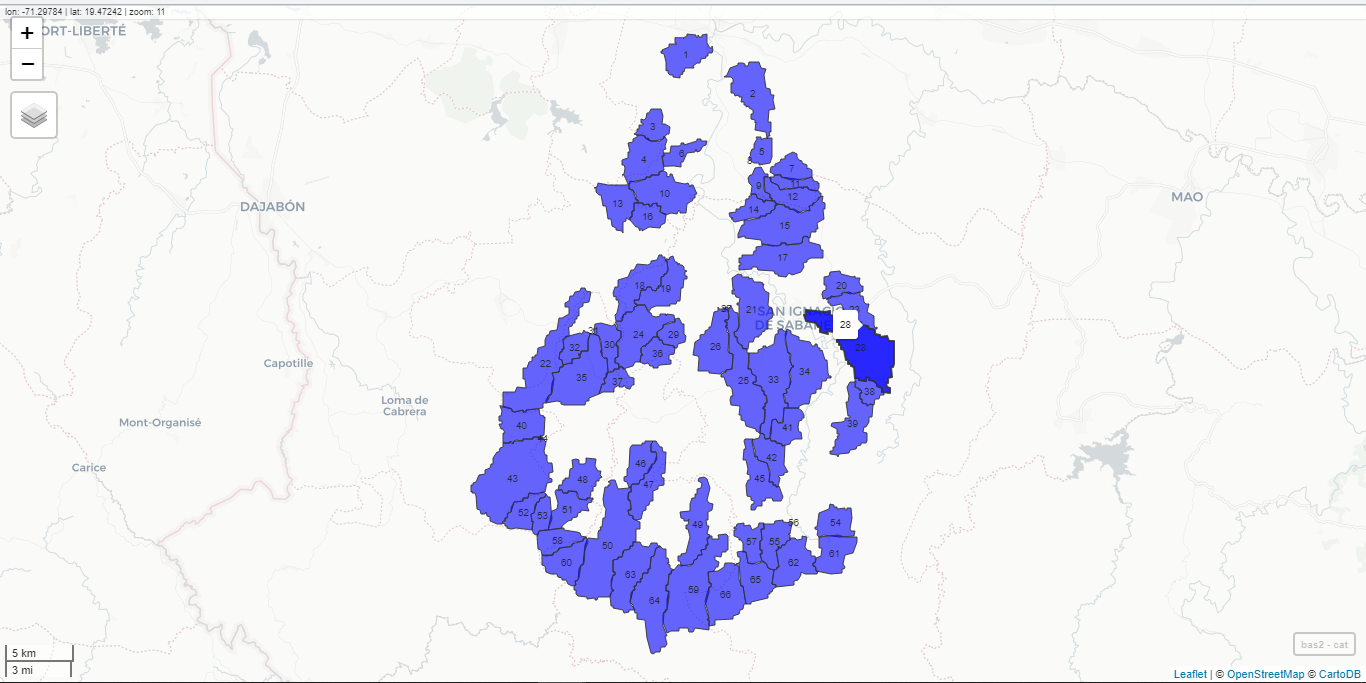
\includegraphics[width=0.90000\textwidth]{Mapview_hypsobasinorder2.png}
\caption{Cuencas de red de drenaje orden 2\label{hypb2}}
\end{figure}

\begin{figure}
\centering
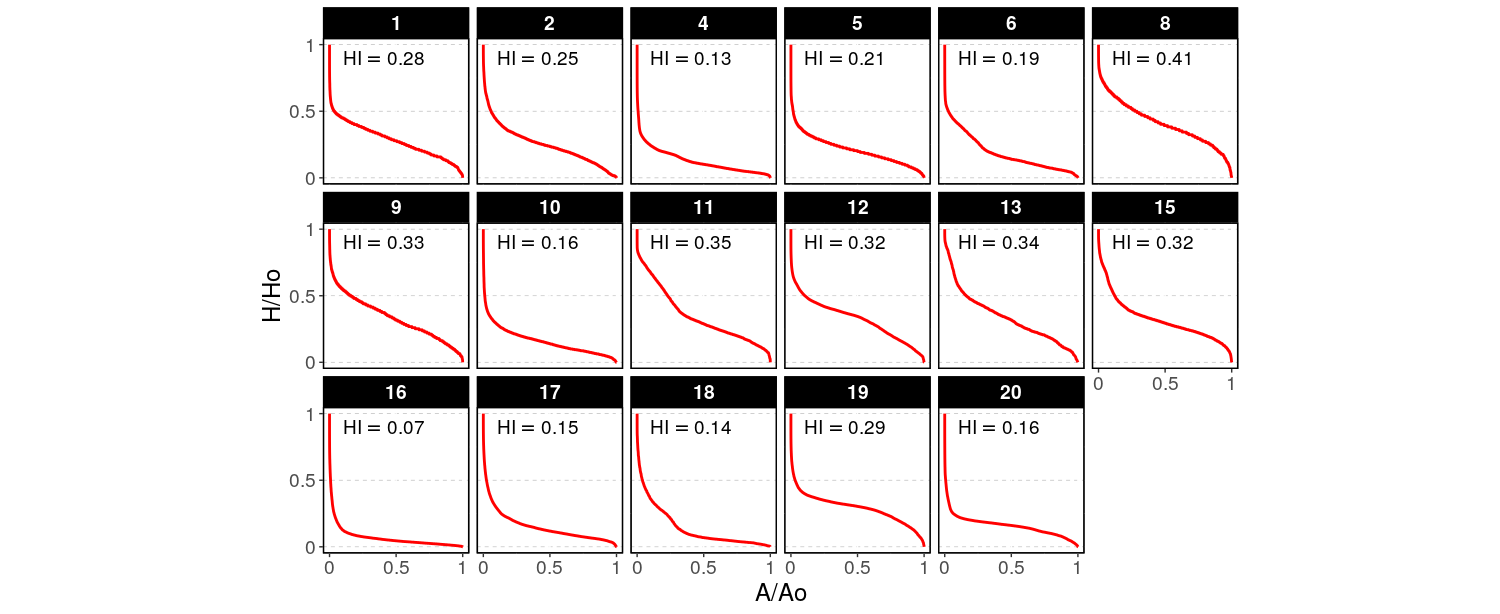
\includegraphics[width=0.80000\textwidth]{HypsoBasinOrder3.png}
\caption{Curva e integral hipsométrica para las cuencas de orden
3\label{hysob3}}
\end{figure}

\begin{figure}
\centering
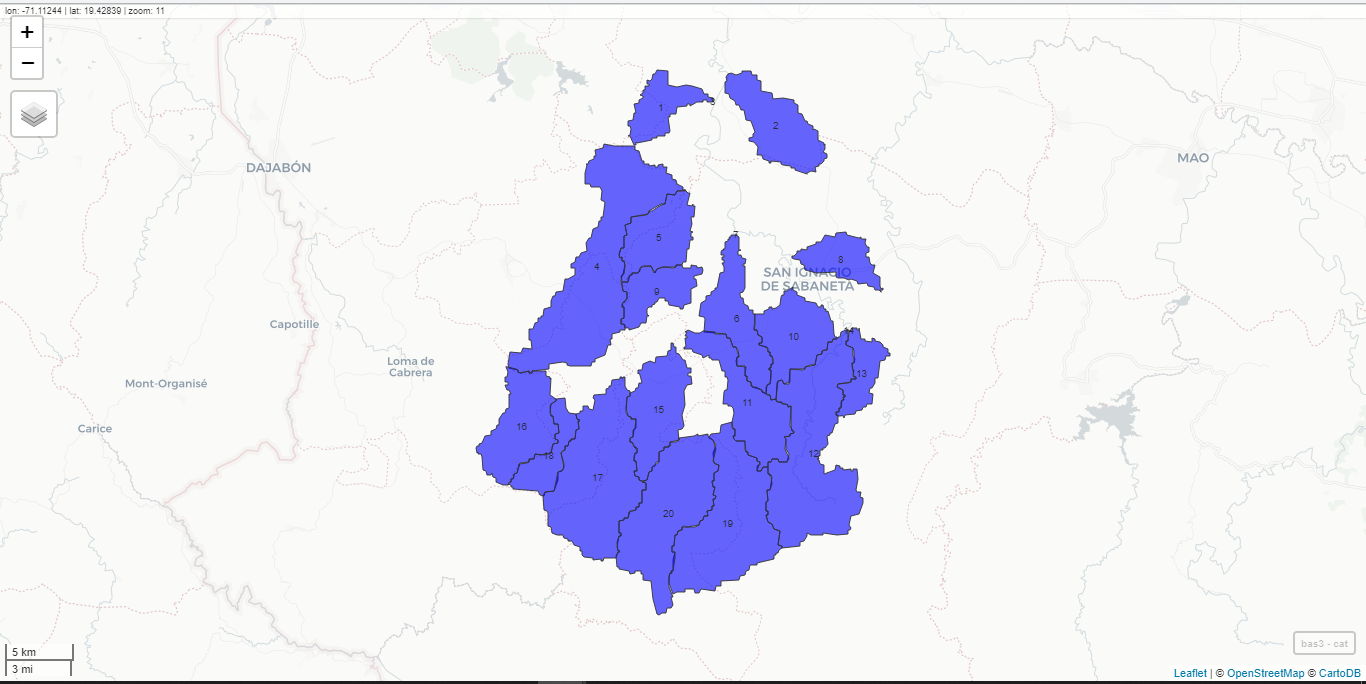
\includegraphics[width=0.90000\textwidth]{Mapview_hypsobasinorder3.png}
\caption{Cuencas de red de drenaje orden 3\label{hypb3}}
\end{figure}

\begin{longtable}[]{@{}cc@{}}
\caption{\label{tab:materiales} Materiales utilizados en la
investigacion.}\tabularnewline
\toprule
\begin{minipage}[b]{0.11\columnwidth}\centering\strut
Materiales\strut
\end{minipage} & \begin{minipage}[b]{0.83\columnwidth}\centering\strut
Uso\strut
\end{minipage}\tabularnewline
\midrule
\endfirsthead
\toprule
\begin{minipage}[b]{0.11\columnwidth}\centering\strut
Materiales\strut
\end{minipage} & \begin{minipage}[b]{0.83\columnwidth}\centering\strut
Uso\strut
\end{minipage}\tabularnewline
\midrule
\endhead
\begin{minipage}[t]{0.11\columnwidth}\centering\strut
RStudio\strut
\end{minipage} & \begin{minipage}[t]{0.83\columnwidth}\centering\strut
Redacción del manuscrito, procesamiento de datos extraídos del MDE de la
cuenca a través de un script.\strut
\end{minipage}\tabularnewline
\begin{minipage}[t]{0.11\columnwidth}\centering\strut
library rgrass7\strut
\end{minipage} & \begin{minipage}[t]{0.83\columnwidth}\centering\strut
Creación de interfaz que establecer conexión entre la version 7 del
sistema de infromacion geográfica GRASS y R, que crea un entorno GRASS
desechable dentro de R.\strut
\end{minipage}\tabularnewline
\begin{minipage}[t]{0.11\columnwidth}\centering\strut
library sp\strut
\end{minipage} & \begin{minipage}[t]{0.83\columnwidth}\centering\strut
Importación, manipulación y exportación de datos espaciales en R, e
impresión de los mismos.\strut
\end{minipage}\tabularnewline
\begin{minipage}[t]{0.11\columnwidth}\centering\strut
library sf\strut
\end{minipage} & \begin{minipage}[t]{0.83\columnwidth}\centering\strut
Creación de caracteristicas simples (simple features), que amplían los
objetos tipo data.frame con una columna de lista de características
simples.\strut
\end{minipage}\tabularnewline
\begin{minipage}[t]{0.11\columnwidth}\centering\strut
library raster\strut
\end{minipage} & \begin{minipage}[t]{0.83\columnwidth}\centering\strut
Manipulación de datos geográficos (espaciales) en formato
`ráster'.\strut
\end{minipage}\tabularnewline
\begin{minipage}[t]{0.11\columnwidth}\centering\strut
library leaflet\strut
\end{minipage} & \begin{minipage}[t]{0.83\columnwidth}\centering\strut
Representación de los vectores y rásters.\strut
\end{minipage}\tabularnewline
\begin{minipage}[t]{0.11\columnwidth}\centering\strut
library leafem\strut
\end{minipage} & \begin{minipage}[t]{0.83\columnwidth}\centering\strut
Proveedor de extensión para leaflet usados para paquetes mapview,
permitió mostrar las coordenadas de la posición del puntero del
mouse.\strut
\end{minipage}\tabularnewline
\begin{minipage}[t]{0.11\columnwidth}\centering\strut
library mapview\strut
\end{minipage} & \begin{minipage}[t]{0.83\columnwidth}\centering\strut
Permitió ver los objetos espaciales de forma interactiva.\strut
\end{minipage}\tabularnewline
\begin{minipage}[t]{0.11\columnwidth}\centering\strut
library readr\strut
\end{minipage} & \begin{minipage}[t]{0.83\columnwidth}\centering\strut
Lector de datos rectangulares (como `csv', `tsv' y `fwf').\strut
\end{minipage}\tabularnewline
\begin{minipage}[t]{0.11\columnwidth}\centering\strut
QGIS with GRASS\strut
\end{minipage} & \begin{minipage}[t]{0.83\columnwidth}\centering\strut
Visualizador de vectores y rasters generados con RStudio en una región
de GRASS, de los mapas Topográfico y Geológico de la República
Dominicana, y, también, Creador de mapas de localización.\strut
\end{minipage}\tabularnewline
\begin{minipage}[t]{0.11\columnwidth}\centering\strut
Google Earth\strut
\end{minipage} & \begin{minipage}[t]{0.83\columnwidth}\centering\strut
Utilizado para observar datos en formato kml generados y exportados de
RStudio y asi como para la representación del relieve del lugar de
estudio.\strut
\end{minipage}\tabularnewline
\begin{minipage}[t]{0.11\columnwidth}\centering\strut
Mapa Topográfico de RD\strut
\end{minipage} & \begin{minipage}[t]{0.83\columnwidth}\centering\strut
Mapa para hacer comparaciones y obtener referencias sobre el
relieve.\strut
\end{minipage}\tabularnewline
\begin{minipage}[t]{0.11\columnwidth}\centering\strut
Mapa Geológico Nacional de RD\strut
\end{minipage} & \begin{minipage}[t]{0.83\columnwidth}\centering\strut
Mapa para hacer comparaciones y obtener referencias sobre la composición
rocosa y los años que datan estas (ver figura\ref{geologico}).\strut
\end{minipage}\tabularnewline
\bottomrule
\end{longtable}

\begin{longtable}[]{@{}cccccc@{}}
\caption{\label{tab:estadisticaor} Estadísticas de los ordenes de red
del río Guayubín}\tabularnewline
\toprule
Max order & Tot.N.str. & Tot.str.len. & Tot.area. & Dr.dens. &
Str.freq.\tabularnewline
\midrule
\endfirsthead
\toprule
Max order & Tot.N.str. & Tot.str.len. & Tot.area. & Dr.dens. &
Str.freq.\tabularnewline
\midrule
\endhead
(num) & (num) & (km) & (km\textsuperscript{2}) &
(km/km\textsuperscript{2}) & (num/km\textsuperscript{2})\tabularnewline
5 & 367 & 693.6069 & 773.2235 & 0.8970 & 0.4746\tabularnewline
\bottomrule
\end{longtable}

\begin{longtable}[]{@{}ccccc@{}}
\caption{\label{tab:regresionc} Razones de cursos basados en el
coeficiente de regresion}\tabularnewline
\toprule
Bif.rt. & Len.rt. & Area.rt. & Slo.rt. & Grd.rt.\tabularnewline
\midrule
\endfirsthead
\toprule
Bif.rt. & Len.rt. & Area.rt. & Slo.rt. & Grd.rt.\tabularnewline
\midrule
\endhead
4.0643 & 2.2928 & 4.5845 & 1.4798 & 1.8338\tabularnewline
\bottomrule
\end{longtable}

\begin{longtable}[]{@{}ccccc@{}}
\caption{\label{tab:estandard} Relaciones de flujo promediadas con
desviaciones estándar}\tabularnewline
\toprule
Bif.rt. & Len.rt. & Area.rt. & Slo.rt. & Grd.rt.\tabularnewline
\midrule
\endfirsthead
\toprule
Bif.rt. & Len.rt. & Area.rt. & Slo.rt. & Grd.rt.\tabularnewline
\midrule
\endhead
4.1235 & 2.3822 & 3.3126 & 1.4938 & 1.9010\tabularnewline
0.4476 & 0.6025 & 2.2153 & 0.0960 & 0.5050\tabularnewline
\bottomrule
\end{longtable}

\begin{longtable}[]{@{}cccccc@{}}
\caption{\label{tab:promo} Variables promediadas para cada orden de
red}\tabularnewline
\toprule
\begin{minipage}[b]{0.08\columnwidth}\centering\strut
Order num\strut
\end{minipage} & \begin{minipage}[b]{0.11\columnwidth}\centering\strut
Avg.len (km)\strut
\end{minipage} & \begin{minipage}[b]{0.25\columnwidth}\centering\strut
Avg.ar (km\textsuperscript{2})\strut
\end{minipage} & \begin{minipage}[b]{0.11\columnwidth}\centering\strut
Avg.sl (m/m)\strut
\end{minipage} & \begin{minipage}[b]{0.14\columnwidth}\centering\strut
Avg.grad. (m/m)\strut
\end{minipage} & \begin{minipage}[b]{0.13\columnwidth}\centering\strut
Avg.el.dif (m)\strut
\end{minipage}\tabularnewline
\midrule
\endfirsthead
\toprule
\begin{minipage}[b]{0.08\columnwidth}\centering\strut
Order num\strut
\end{minipage} & \begin{minipage}[b]{0.11\columnwidth}\centering\strut
Avg.len (km)\strut
\end{minipage} & \begin{minipage}[b]{0.25\columnwidth}\centering\strut
Avg.ar (km\textsuperscript{2})\strut
\end{minipage} & \begin{minipage}[b]{0.11\columnwidth}\centering\strut
Avg.sl (m/m)\strut
\end{minipage} & \begin{minipage}[b]{0.14\columnwidth}\centering\strut
Avg.grad. (m/m)\strut
\end{minipage} & \begin{minipage}[b]{0.13\columnwidth}\centering\strut
Avg.el.dif (m)\strut
\end{minipage}\tabularnewline
\midrule
\endhead
\begin{minipage}[t]{0.08\columnwidth}\centering\strut
1\strut
\end{minipage} & \begin{minipage}[t]{0.11\columnwidth}\centering\strut
1.2435\strut
\end{minipage} & \begin{minipage}[t]{0.25\columnwidth}\centering\strut
1.7188\strut
\end{minipage} & \begin{minipage}[t]{0.11\columnwidth}\centering\strut
0.0367\strut
\end{minipage} & \begin{minipage}[t]{0.14\columnwidth}\centering\strut
0.0296\strut
\end{minipage} & \begin{minipage}[t]{0.13\columnwidth}\centering\strut
37.4437\strut
\end{minipage}\tabularnewline
\begin{minipage}[t]{0.08\columnwidth}\centering\strut
2\strut
\end{minipage} & \begin{minipage}[t]{0.11\columnwidth}\centering\strut
2.4743\strut
\end{minipage} & \begin{minipage}[t]{0.25\columnwidth}\centering\strut
7.2904\strut
\end{minipage} & \begin{minipage}[t]{0.11\columnwidth}\centering\strut
0.0246\strut
\end{minipage} & \begin{minipage}[t]{0.14\columnwidth}\centering\strut
0.0201\strut
\end{minipage} & \begin{minipage}[t]{0.13\columnwidth}\centering\strut
49.0820\strut
\end{minipage}\tabularnewline
\begin{minipage}[t]{0.08\columnwidth}\centering\strut
3\strut
\end{minipage} & \begin{minipage}[t]{0.11\columnwidth}\centering\strut
6.2881\strut
\end{minipage} & \begin{minipage}[t]{0.25\columnwidth}\centering\strut
31.7328\strut
\end{minipage} & \begin{minipage}[t]{0.11\columnwidth}\centering\strut
0.0165\strut
\end{minipage} & \begin{minipage}[t]{0.14\columnwidth}\centering\strut
0.0113\strut
\end{minipage} & \begin{minipage}[t]{0.13\columnwidth}\centering\strut
85.1765\strut
\end{minipage}\tabularnewline
\begin{minipage}[t]{0.08\columnwidth}\centering\strut
4\strut
\end{minipage} & \begin{minipage}[t]{0.11\columnwidth}\centering\strut
11.5356\strut
\end{minipage} & \begin{minipage}[t]{0.25\columnwidth}\centering\strut
147.7492\strut
\end{minipage} & \begin{minipage}[t]{0.11\columnwidth}\centering\strut
0.0120\strut
\end{minipage} & \begin{minipage}[t]{0.14\columnwidth}\centering\strut
0.0066\strut
\end{minipage} & \begin{minipage}[t]{0.13\columnwidth}\centering\strut
80.0000\strut
\end{minipage}\tabularnewline
\begin{minipage}[t]{0.08\columnwidth}\centering\strut
5\strut
\end{minipage} & \begin{minipage}[t]{0.11\columnwidth}\centering\strut
36.4888\strut
\end{minipage} & \begin{minipage}[t]{0.25\columnwidth}\centering\strut
773.2235\strut
\end{minipage} & \begin{minipage}[t]{0.11\columnwidth}\centering\strut
0.0074\strut
\end{minipage} & \begin{minipage}[t]{0.14\columnwidth}\centering\strut
0.0025\strut
\end{minipage} & \begin{minipage}[t]{0.13\columnwidth}\centering\strut
91.0000\strut
\end{minipage}\tabularnewline
\bottomrule
\end{longtable}

\begin{longtable}[]{@{}cccccc@{}}
\caption{\label{tab:estad} Desviacion estandar para las estadisticas
segun orden de red}\tabularnewline
\toprule
\begin{minipage}[b]{0.08\columnwidth}\centering\strut
Order num\strut
\end{minipage} & \begin{minipage}[b]{0.11\columnwidth}\centering\strut
Std.len (km)\strut
\end{minipage} & \begin{minipage}[b]{0.26\columnwidth}\centering\strut
Std.ar (km\textsuperscript{2})\strut
\end{minipage} & \begin{minipage}[b]{0.11\columnwidth}\centering\strut
Std.sl (m/m)\strut
\end{minipage} & \begin{minipage}[b]{0.14\columnwidth}\centering\strut
Std.grad. (m/m)\strut
\end{minipage} & \begin{minipage}[b]{0.13\columnwidth}\centering\strut
Std.el.dif (m)\strut
\end{minipage}\tabularnewline
\midrule
\endfirsthead
\toprule
\begin{minipage}[b]{0.08\columnwidth}\centering\strut
Order num\strut
\end{minipage} & \begin{minipage}[b]{0.11\columnwidth}\centering\strut
Std.len (km)\strut
\end{minipage} & \begin{minipage}[b]{0.26\columnwidth}\centering\strut
Std.ar (km\textsuperscript{2})\strut
\end{minipage} & \begin{minipage}[b]{0.11\columnwidth}\centering\strut
Std.sl (m/m)\strut
\end{minipage} & \begin{minipage}[b]{0.14\columnwidth}\centering\strut
Std.grad. (m/m)\strut
\end{minipage} & \begin{minipage}[b]{0.13\columnwidth}\centering\strut
Std.el.dif (m)\strut
\end{minipage}\tabularnewline
\midrule
\endhead
\begin{minipage}[t]{0.08\columnwidth}\centering\strut
1\strut
\end{minipage} & \begin{minipage}[t]{0.11\columnwidth}\centering\strut
1.0274\strut
\end{minipage} & \begin{minipage}[t]{0.26\columnwidth}\centering\strut
1.0955\strut
\end{minipage} & \begin{minipage}[t]{0.11\columnwidth}\centering\strut
0.0379\strut
\end{minipage} & \begin{minipage}[t]{0.14\columnwidth}\centering\strut
0.0324\strut
\end{minipage} & \begin{minipage}[t]{0.13\columnwidth}\centering\strut
52.7742\strut
\end{minipage}\tabularnewline
\begin{minipage}[t]{0.08\columnwidth}\centering\strut
2\strut
\end{minipage} & \begin{minipage}[t]{0.11\columnwidth}\centering\strut
1.9695\strut
\end{minipage} & \begin{minipage}[t]{0.26\columnwidth}\centering\strut
4.4097\strut
\end{minipage} & \begin{minipage}[t]{0.11\columnwidth}\centering\strut
0.0215\strut
\end{minipage} & \begin{minipage}[t]{0.14\columnwidth}\centering\strut
0.0194\strut
\end{minipage} & \begin{minipage}[t]{0.13\columnwidth}\centering\strut
52.5830\strut
\end{minipage}\tabularnewline
\begin{minipage}[t]{0.08\columnwidth}\centering\strut
3\strut
\end{minipage} & \begin{minipage}[t]{0.11\columnwidth}\centering\strut
5.0992\strut
\end{minipage} & \begin{minipage}[t]{0.26\columnwidth}\centering\strut
19.0637\strut
\end{minipage} & \begin{minipage}[t]{0.11\columnwidth}\centering\strut
0.0092\strut
\end{minipage} & \begin{minipage}[t]{0.14\columnwidth}\centering\strut
0.0077\strut
\end{minipage} & \begin{minipage}[t]{0.13\columnwidth}\centering\strut
93.4085\strut
\end{minipage}\tabularnewline
\begin{minipage}[t]{0.08\columnwidth}\centering\strut
4\strut
\end{minipage} & \begin{minipage}[t]{0.11\columnwidth}\centering\strut
5.8247\strut
\end{minipage} & \begin{minipage}[t]{0.26\columnwidth}\centering\strut
44.3177\strut
\end{minipage} & \begin{minipage}[t]{0.11\columnwidth}\centering\strut
0.0041\strut
\end{minipage} & \begin{minipage}[t]{0.14\columnwidth}\centering\strut
0.0032\strut
\end{minipage} & \begin{minipage}[t]{0.13\columnwidth}\centering\strut
57.0789\strut
\end{minipage}\tabularnewline
\begin{minipage}[t]{0.08\columnwidth}\centering\strut
5\strut
\end{minipage} & \begin{minipage}[t]{0.11\columnwidth}\centering\strut
-0.0000\strut
\end{minipage} & \begin{minipage}[t]{0.26\columnwidth}\centering\strut
0.0000\strut
\end{minipage} & \begin{minipage}[t]{0.11\columnwidth}\centering\strut
0.0000\strut
\end{minipage} & \begin{minipage}[t]{0.14\columnwidth}\centering\strut
0.0000\strut
\end{minipage} & \begin{minipage}[t]{0.13\columnwidth}\centering\strut
0.0000\strut
\end{minipage}\tabularnewline
\bottomrule
\end{longtable}

\begin{longtable}[]{@{}cccc@{}}
\caption{\label{tab:parh} Estadisticas de parámetros hidrgográficos
según el orden de red}\tabularnewline
\toprule
Order & N.streams & Tot.len (km) & Tot.area
(km\textsuperscript{2})\tabularnewline
\midrule
\endfirsthead
\toprule
Order & N.streams & Tot.len (km) & Tot.area
(km\textsuperscript{2})\tabularnewline
\midrule
\endhead
1 & 284 & 353.1463 & 488.1383\tabularnewline
2 & 61 & 150.9325 & 444.7173\tabularnewline
3 & 17 & 106.8969 & 539.4576\tabularnewline
4 & 4 & 46.1425 & 590.9969\tabularnewline
5 & 1 & 36.4888 & 773.2235\tabularnewline
\bottomrule
\end{longtable}

\begin{longtable}[]{@{}cccccccc@{}}
\caption{\label{tab:razones} Razones de los parámetros hidrográficos
según su orden de red}\tabularnewline
\toprule
Order & Bif.rt. & Len.rt. & Area.rt. & Slo.rt. & Grd.rt. & d.dens. &
str.freq.\tabularnewline
\midrule
\endfirsthead
\toprule
Order & Bif.rt. & Len.rt. & Area.rt. & Slo.rt. & Grd.rt. & d.dens. &
str.freq.\tabularnewline
\midrule
\endhead
1 & 4.6557 & 1.9898 & 0.0000 & 1.4930 & 1.4748 & 0.7235 &
0.5818\tabularnewline
2 & 3.5882 & 2.5413 & 4.2416 & 1.4930 & 1.7757 & 0.3394 &
0.1372\tabularnewline
3 & 4.2500 & 1.8345 & 4.3527 & 1.3771 & 1.7207 & 0.1982 &
0.0315\tabularnewline
4 & 4.0000 & 3.1631 & 4.6560 & 1.6122 & 2.6327 & 0.0781 &
0.0068\tabularnewline
5 & 0.0000 & 0.0000 & 5.2334 & 0.0000 & 0.0000 & 0.0472 &
0.0013\tabularnewline
\bottomrule
\end{longtable}

\begin{longtable}[]{@{}cc@{}}
\caption{\label{tab:parametrosm}Parámetros morfométricos de la cuenca
del río Guayubín.}\tabularnewline
\toprule
\begin{minipage}[b]{0.65\columnwidth}\centering\strut
Parámetros\strut
\end{minipage} & \begin{minipage}[b]{0.29\columnwidth}\centering\strut
Valores\strut
\end{minipage}\tabularnewline
\midrule
\endfirsthead
\toprule
\begin{minipage}[b]{0.65\columnwidth}\centering\strut
Parámetros\strut
\end{minipage} & \begin{minipage}[b]{0.29\columnwidth}\centering\strut
Valores\strut
\end{minipage}\tabularnewline
\midrule
\endhead
\begin{minipage}[t]{0.65\columnwidth}\centering\strut
Easting Centroid of basin\strut
\end{minipage} & \begin{minipage}[t]{0.29\columnwidth}\centering\strut
246465.00\strut
\end{minipage}\tabularnewline
\begin{minipage}[t]{0.65\columnwidth}\centering\strut
Northing Centroid of basin\strut
\end{minipage} & \begin{minipage}[t]{0.29\columnwidth}\centering\strut
2151675.00\strut
\end{minipage}\tabularnewline
\begin{minipage}[t]{0.65\columnwidth}\centering\strut
Rectangle containing basin N-W\strut
\end{minipage} & \begin{minipage}[t]{0.29\columnwidth}\centering\strut
(`230220', `2175930')\strut
\end{minipage}\tabularnewline
\begin{minipage}[t]{0.65\columnwidth}\centering\strut
Rectangle containing basin S-E\strut
\end{minipage} & \begin{minipage}[t]{0.29\columnwidth}\centering\strut
(`261000', `2131290')\strut
\end{minipage}\tabularnewline
\begin{minipage}[t]{0.65\columnwidth}\centering\strut
Area of basin {[}km\textsuperscript{2}{]}\strut
\end{minipage} & \begin{minipage}[t]{0.29\columnwidth}\centering\strut
773.5631625\strut
\end{minipage}\tabularnewline
\begin{minipage}[t]{0.65\columnwidth}\centering\strut
Perimeter of basin {[}km{]}\strut
\end{minipage} & \begin{minipage}[t]{0.29\columnwidth}\centering\strut
156.122652506552\strut
\end{minipage}\tabularnewline
\begin{minipage}[t]{0.65\columnwidth}\centering\strut
Max Elevation {[}m s.l.m.{]}\strut
\end{minipage} & \begin{minipage}[t]{0.29\columnwidth}\centering\strut
1396.72540740785\strut
\end{minipage}\tabularnewline
\begin{minipage}[t]{0.65\columnwidth}\centering\strut
Min Elevation {[}m s.l.m.{]}\strut
\end{minipage} & \begin{minipage}[t]{0.29\columnwidth}\centering\strut
30.9651954818271\strut
\end{minipage}\tabularnewline
\begin{minipage}[t]{0.65\columnwidth}\centering\strut
Elevation Difference {[}m{]}\strut
\end{minipage} & \begin{minipage}[t]{0.29\columnwidth}\centering\strut
1365.760211926023\strut
\end{minipage}\tabularnewline
\begin{minipage}[t]{0.65\columnwidth}\centering\strut
Mean Elevation\strut
\end{minipage} & \begin{minipage}[t]{0.29\columnwidth}\centering\strut
276.7019\strut
\end{minipage}\tabularnewline
\begin{minipage}[t]{0.65\columnwidth}\centering\strut
Mean Slope\strut
\end{minipage} & \begin{minipage}[t]{0.29\columnwidth}\centering\strut
5.17\strut
\end{minipage}\tabularnewline
\begin{minipage}[t]{0.65\columnwidth}\centering\strut
Length of Directing Vector {[}km{]}\strut
\end{minipage} & \begin{minipage}[t]{0.29\columnwidth}\centering\strut
24.460893544594807\strut
\end{minipage}\tabularnewline
\begin{minipage}[t]{0.65\columnwidth}\centering\strut
Prevalent Orientation {[}degree from north, counterclockwise{]}\strut
\end{minipage} & \begin{minipage}[t]{0.29\columnwidth}\centering\strut
1.4935760627096282\strut
\end{minipage}\tabularnewline
\begin{minipage}[t]{0.65\columnwidth}\centering\strut
Compactness Coefficient\strut
\end{minipage} & \begin{minipage}[t]{0.29\columnwidth}\centering\strut
4.974655054098116\strut
\end{minipage}\tabularnewline
\begin{minipage}[t]{0.65\columnwidth}\centering\strut
Circularity Ratio\strut
\end{minipage} & \begin{minipage}[t]{0.29\columnwidth}\centering\strut
0.3988171279899944\strut
\end{minipage}\tabularnewline
\begin{minipage}[t]{0.65\columnwidth}\centering\strut
Topological Diameter\strut
\end{minipage} & \begin{minipage}[t]{0.29\columnwidth}\centering\strut
84.0\strut
\end{minipage}\tabularnewline
\begin{minipage}[t]{0.65\columnwidth}\centering\strut
Elongation Ratio\strut
\end{minipage} & \begin{minipage}[t]{0.29\columnwidth}\centering\strut
0.5064682945330589\strut
\end{minipage}\tabularnewline
\begin{minipage}[t]{0.65\columnwidth}\centering\strut
Shape Factor\strut
\end{minipage} & \begin{minipage}[t]{0.29\columnwidth}\centering\strut
12.483750895456415\strut
\end{minipage}\tabularnewline
\begin{minipage}[t]{0.65\columnwidth}\centering\strut
Concentration Time (Giandotti, 1934) {[}hr{]}\strut
\end{minipage} & \begin{minipage}[t]{0.29\columnwidth}\centering\strut
6.906840311938352\strut
\end{minipage}\tabularnewline
\begin{minipage}[t]{0.65\columnwidth}\centering\strut
Length of Mainchannel {[}km{]}\strut
\end{minipage} & \begin{minipage}[t]{0.29\columnwidth}\centering\strut
61.965603846\strut
\end{minipage}\tabularnewline
\begin{minipage}[t]{0.65\columnwidth}\centering\strut
Mean slope of mainchannel {[}percent{]}\strut
\end{minipage} & \begin{minipage}[t]{0.29\columnwidth}\centering\strut
1.9669190473941982\strut
\end{minipage}\tabularnewline
\begin{minipage}[t]{0.65\columnwidth}\centering\strut
Mean hillslope length {[}m{]}\strut
\end{minipage} & \begin{minipage}[t]{0.29\columnwidth}\centering\strut
250.4986\strut
\end{minipage}\tabularnewline
\begin{minipage}[t]{0.65\columnwidth}\centering\strut
Magnitudo\strut
\end{minipage} & \begin{minipage}[t]{0.29\columnwidth}\centering\strut
223.0\strut
\end{minipage}\tabularnewline
\begin{minipage}[t]{0.65\columnwidth}\centering\strut
Max order (Strahler)\strut
\end{minipage} & \begin{minipage}[t]{0.29\columnwidth}\centering\strut
5\strut
\end{minipage}\tabularnewline
\begin{minipage}[t]{0.65\columnwidth}\centering\strut
Number of streams\strut
\end{minipage} & \begin{minipage}[t]{0.29\columnwidth}\centering\strut
343\strut
\end{minipage}\tabularnewline
\begin{minipage}[t]{0.65\columnwidth}\centering\strut
Total Stream Length {[}km{]}\strut
\end{minipage} & \begin{minipage}[t]{0.29\columnwidth}\centering\strut
662.2185\strut
\end{minipage}\tabularnewline
\begin{minipage}[t]{0.65\columnwidth}\centering\strut
First order stream frequency\strut
\end{minipage} & \begin{minipage}[t]{0.29\columnwidth}\centering\strut
0.2882763952710843\strut
\end{minipage}\tabularnewline
\begin{minipage}[t]{0.65\columnwidth}\centering\strut
Drainage Density {[}km/km\textsuperscript{2}{]}\strut
\end{minipage} & \begin{minipage}[t]{0.29\columnwidth}\centering\strut
0.8560626101427108\strut
\end{minipage}\tabularnewline
\begin{minipage}[t]{0.65\columnwidth}\centering\strut
Bifurcation Ratio (Horton)\strut
\end{minipage} & \begin{minipage}[t]{0.29\columnwidth}\centering\strut
3.8876\strut
\end{minipage}\tabularnewline
\begin{minipage}[t]{0.65\columnwidth}\centering\strut
Length Ratio (Horton)\strut
\end{minipage} & \begin{minipage}[t]{0.29\columnwidth}\centering\strut
2.2966\strut
\end{minipage}\tabularnewline
\begin{minipage}[t]{0.65\columnwidth}\centering\strut
Area ratio (Horton)\strut
\end{minipage} & \begin{minipage}[t]{0.29\columnwidth}\centering\strut
4.3704\strut
\end{minipage}\tabularnewline
\begin{minipage}[t]{0.65\columnwidth}\centering\strut
Slope ratio (Horton)\strut
\end{minipage} & \begin{minipage}[t]{0.29\columnwidth}\centering\strut
1.4689\strut
\end{minipage}\tabularnewline
\bottomrule
\end{longtable}

\begin{longtable}[]{@{}cc@{}}
\caption{\label{tab:ihco2} Integral hipsométrica en las cuencas de orden
2}\tabularnewline
\toprule
Categoría & Integral hipsométrica\tabularnewline
\midrule
\endfirsthead
\toprule
Categoría & Integral hipsométrica\tabularnewline
\midrule
\endhead
1 & 0.23784092\tabularnewline
2 & 0.29691935\tabularnewline
3 & 0.31478851\tabularnewline
4 & 0.25845620\tabularnewline
5 & 0.18914104\tabularnewline
6 & 0.38449116\tabularnewline
7 & 0.25087104\tabularnewline
9 & 0.26943542\tabularnewline
10 & 0.19779399\tabularnewline
11 & 0.19287436\tabularnewline
12 & 0.17808813\tabularnewline
13 & 0.22437828\tabularnewline
14 & 0.40595651\tabularnewline
15 & 0.25477715\tabularnewline
16 & 0.19777159\tabularnewline
17 & 0.25313336\tabularnewline
18 & 0.22679929\tabularnewline
19 & 0.30597060\tabularnewline
20 & 0.30564285\tabularnewline
21 & 0.24773997\tabularnewline
22 & 0.21800099\tabularnewline
23 & 0.33229314\tabularnewline
24 & 0.40758028\tabularnewline
25 & 0.27096759\tabularnewline
26 & 0.17485732\tabularnewline
28 & 0.25721054\tabularnewline
29 & 0.27907973\tabularnewline
30 & 0.23545394\tabularnewline
32 & 0.24544610\tabularnewline
33 & 0.18990261\tabularnewline
34 & 0.22303577\tabularnewline
35 & 0.14436574\tabularnewline
36 & 0.30229714\tabularnewline
37 & 0.30742281\tabularnewline
38 & 0.34876647\tabularnewline
39 & 0.39371293\tabularnewline
40 & 0.14419677\tabularnewline
41 & 0.36397062\tabularnewline
42 & 0.45795809\tabularnewline
43 & 0.07642614\tabularnewline
45 & 0.48672629\tabularnewline
46 & 0.29182502\tabularnewline
47 & 0.47300056\tabularnewline
48 & 0.22892086\tabularnewline
49 & 0.50910119\tabularnewline
50 & 0.16011357\tabularnewline
51 & 0.14325914\tabularnewline
52 & 0.30243670\tabularnewline
53 & 0.22622911\tabularnewline
54 & 0.27985062\tabularnewline
55 & 0.16980308\tabularnewline
57 & 0.38363564\tabularnewline
58 & 0.29000326\tabularnewline
59 & 0.23691203\tabularnewline
60 & 0.30564446\tabularnewline
61 & 0.30401039\tabularnewline
62 & 0.25939942\tabularnewline
63 & 0.16711030\tabularnewline
64 & 0.14693431\tabularnewline
65 & 0.19359746\tabularnewline
66 & 0.17854689\tabularnewline
\bottomrule
\end{longtable}

\begin{longtable}[]{@{}cc@{}}
\caption{\label{tab:ihco3} Integral hipsométrica en las cuencas de orden
3}\tabularnewline
\toprule
Categoría & Integral hipsométrico\tabularnewline
\midrule
\endfirsthead
\toprule
Categoría & Integral hipsométrico\tabularnewline
\midrule
\endhead
1 & 0.28106607\tabularnewline
2 & 0.24855493\tabularnewline
4 & 0.12697883\tabularnewline
5 & 0.21021494\tabularnewline
6 & 0.18586633\tabularnewline
8 & 0.40849637\tabularnewline
9 & 0.33264116\tabularnewline
10 & 0.15880640\tabularnewline
11 & 0.34507681\tabularnewline
12 & 0.32371339\tabularnewline
13 & 0.33707592\tabularnewline
15 & 0.32319904\tabularnewline
16 & 0.06673204\tabularnewline
17 & 0.15091492\tabularnewline
18 & 0.14111015\tabularnewline
19 & 0.29051932\tabularnewline
20 & 0.15859746\tabularnewline
\bottomrule
\end{longtable}

\section{\texorpdfstring{\emph{Script}
reproducible}{Script reproducible}}\label{script-reproducible}

\begin{Shaded}
\begin{Highlighting}[]
\CommentTok{# Intro a Grass, video no. 3 ----}
\NormalTok{## Parte reutilizable del script ----}
\NormalTok{## Cargar paquetes}
\KeywordTok{library}\NormalTok{(rgrass7)}
\KeywordTok{library}\NormalTok{(sp)}
\KeywordTok{use_sp}\NormalTok{()}
\KeywordTok{library}\NormalTok{(sf)}
\KeywordTok{library}\NormalTok{(raster)}
\KeywordTok{library}\NormalTok{(leaflet)}
\KeywordTok{library}\NormalTok{(leafem)}
\KeywordTok{library}\NormalTok{(mapview)}
\KeywordTok{library}\NormalTok{(readr)}

\NormalTok{gisdbase <-}\StringTok{ 'grass-data-test'} \CommentTok{#Base de datos de GRASS GIS}
\NormalTok{wd <-}\StringTok{ }\KeywordTok{getwd}\NormalTok{() }\CommentTok{#Directorio de trabajo}
\NormalTok{wd}
\NormalTok{loc <-}\StringTok{ }\KeywordTok{initGRASS}\NormalTok{(}\DataTypeTok{gisBase =} \StringTok{"/usr/lib/grass78/"}\NormalTok{,}
                 \DataTypeTok{home =}\NormalTok{ wd,}
                 \DataTypeTok{gisDbase =} \KeywordTok{paste}\NormalTok{(wd, gisdbase, }\DataTypeTok{sep =} \StringTok{'/'}\NormalTok{),}
                 \DataTypeTok{location =} \StringTok{'guayubin'}\NormalTok{,}
                 \DataTypeTok{mapset =} \StringTok{"PERMANENT"}\NormalTok{,}
                 \DataTypeTok{override =} \OtherTok{TRUE}\NormalTok{)}

\NormalTok{## Imprimir fuentes en la region}
\KeywordTok{execGRASS}\NormalTok{(}
  \StringTok{'g.list'}\NormalTok{,}
  \DataTypeTok{flags =} \StringTok{'t'}\NormalTok{,}
  \DataTypeTok{parameters =} \KeywordTok{list}\NormalTok{(}
    \DataTypeTok{type =} \KeywordTok{c}\NormalTok{(}\StringTok{'raster'}\NormalTok{, }\StringTok{'vector'}\NormalTok{)}
\NormalTok{  )}
\NormalTok{)}

\NormalTok{## Limpiar archivo de bloqueo del conjunto de mapas de GRASS}
\KeywordTok{unlink_.gislock}\NormalTok{()}

\NormalTok{## Fin de la parte reutilizable}

\CommentTok{# Video no. 4, Definir proyección de la región de GRASS GIS, importar fuente y utilizarla para definir extensión y resolución. Cómo ver la ayuda de las funciones ----}
\NormalTok{## Muestra la definición de la región}
\KeywordTok{gmeta}\NormalTok{()}

\NormalTok{## Definir ruta del DEM}
\NormalTok{dem <-}\StringTok{ 'datos-fuente/srtm_dem_cuenca_guayubin.tif'}
\KeywordTok{execGRASS}\NormalTok{(}
  \DataTypeTok{cmd =} \StringTok{'g.proj'}\NormalTok{,}
  \DataTypeTok{flags =} \KeywordTok{c}\NormalTok{(}\StringTok{'t'}\NormalTok{,}\StringTok{'c'}\NormalTok{),}
  \DataTypeTok{georef =}\NormalTok{ dem)}

\NormalTok{## Muestra la definición de la región modificada}
\KeywordTok{gmeta}\NormalTok{()}

\NormalTok{## r.in.gdal importa la fuente a GRASS}
\KeywordTok{execGRASS}\NormalTok{(}
  \DataTypeTok{cmd =} \StringTok{'r.in.gdal'}\NormalTok{,}
  \DataTypeTok{flags=}\KeywordTok{c}\NormalTok{(}\StringTok{'overwrite'}\NormalTok{,}\StringTok{'quiet'}\NormalTok{),}
  \DataTypeTok{parameters=}\KeywordTok{list}\NormalTok{(}
    \DataTypeTok{input=}\NormalTok{dem,}
    \DataTypeTok{output=}\StringTok{'dem'}
\NormalTok{  )}
\NormalTok{)}

\NormalTok{## Actualizar la extensión de la región al DEM, sólo por precaución}
\KeywordTok{execGRASS}\NormalTok{(}
  \DataTypeTok{cmd =} \StringTok{'g.region'}\NormalTok{,}
  \DataTypeTok{parameters=}\KeywordTok{list}\NormalTok{(}
    \DataTypeTok{raster =} \StringTok{'dem'}\NormalTok{,}
    \DataTypeTok{align =} \StringTok{'dem'}
\NormalTok{  )}
\NormalTok{)}

\NormalTok{## Muestra la región de Grass again}
\KeywordTok{gmeta}\NormalTok{()}

\NormalTok{## Importar vectorial a la región de Grass}
\NormalTok{demext <-}\StringTok{ 'datos-fuente/srtm_dem_cuenca_guayubin.geojson'}
\KeywordTok{execGRASS}\NormalTok{(}
  \DataTypeTok{cmd =} \StringTok{'v.in.ogr'}\NormalTok{,}
  \DataTypeTok{flags=}\KeywordTok{c}\NormalTok{(}\StringTok{'overwrite'}\NormalTok{,}\StringTok{'quiet'}\NormalTok{),}
  \DataTypeTok{parameters=}\KeywordTok{list}\NormalTok{(}
    \DataTypeTok{input =}\NormalTok{ demext,}
    \DataTypeTok{output =} \StringTok{'dem_extent'}
\NormalTok{  )}
\NormalTok{)}

\NormalTok{## Imprimir lista de mapas ráster y vectoriales dentro en la región/localización activa}
\KeywordTok{execGRASS}\NormalTok{(}
  \StringTok{'g.list'}\NormalTok{,}
  \DataTypeTok{flags =} \StringTok{'t'}\NormalTok{,}
  \DataTypeTok{parameters =} \KeywordTok{list}\NormalTok{(}
    \DataTypeTok{type =} \KeywordTok{c}\NormalTok{(}\StringTok{'raster'}\NormalTok{, }\StringTok{'vector'}\NormalTok{)}
\NormalTok{  )}
\NormalTok{)}

\NormalTok{## Ver los addons disponibles en el repositorio oficial de GRASS GIS, incluyendo descripción}
\KeywordTok{execGRASS}\NormalTok{(}
  \DataTypeTok{cmd =} \StringTok{'g.extension'}\NormalTok{,}
  \DataTypeTok{flags =} \StringTok{'c'}
\NormalTok{)}

\NormalTok{## Consultar la ayuda de una función}
\KeywordTok{parseGRASS}\NormalTok{(}\StringTok{"r.in.gdal"}\NormalTok{)}

\NormalTok{## Consultar la ayuda de una función. Segunda alternativa}
\KeywordTok{system}\NormalTok{(}\StringTok{'r.in.gdal --help'}\NormalTok{)}

\NormalTok{## Limpiar archivo de bloqueo del conjunto de mapas de GRASS}
\KeywordTok{unlink_.gislock}\NormalTok{()}

\CommentTok{# Video no. 5, Explorar datos espaciales básicos entre GRASS y R ----}
\NormalTok{## Imprimir lista de mapas ráster y vectoriales dentro en la región/localización activa}
\KeywordTok{execGRASS}\NormalTok{(}
  \StringTok{'g.list'}\NormalTok{,}
  \DataTypeTok{flags =} \StringTok{'t'}\NormalTok{,}
  \DataTypeTok{parameters =} \KeywordTok{list}\NormalTok{(}
    \DataTypeTok{type =} \KeywordTok{c}\NormalTok{(}\StringTok{'raster'}\NormalTok{, }\StringTok{'vector'}\NormalTok{)}
\NormalTok{  )}
\NormalTok{)}

\NormalTok{## Cargar en R el DEM (mapa ráster)}
\KeywordTok{library}\NormalTok{(sp)}
\KeywordTok{use_sp}\NormalTok{()}
\NormalTok{dem_sp <-}\StringTok{ }\KeywordTok{readRAST}\NormalTok{(}\StringTok{'dem'}\NormalTok{)}
\NormalTok{op <-}\StringTok{ }\KeywordTok{par}\NormalTok{()}
\KeywordTok{plot}\NormalTok{(dem_sp)}

\NormalTok{## Cargar a R el mapa vectorial de una cuenca que se encuentra alojado fuera de GRASS, hacer el plot y representar la cuenca del rio Guayubin superpuesta}
\KeywordTok{library}\NormalTok{(sf)}
\NormalTok{rutaguayubin <-}\StringTok{ 'datos-fuente/cuenca_guayubin.geojson'}
\NormalTok{guayubin <-}\StringTok{ }\KeywordTok{st_read}\NormalTok{(rutaguayubin)}
\KeywordTok{plot}\NormalTok{(dem_sp)}
\KeywordTok{plot}\NormalTok{(guayubin, }\DataTypeTok{add=}\NormalTok{T, }\DataTypeTok{col=}\StringTok{'transparent'}\NormalTok{, }\DataTypeTok{border=}\StringTok{'black'}\NormalTok{, }\DataTypeTok{lwd=}\DecValTok{5}\NormalTok{);}\KeywordTok{par}\NormalTok{(op[}\KeywordTok{c}\NormalTok{(}\StringTok{'mfrow'}\NormalTok{,}\StringTok{'mar'}\NormalTok{)])}

\NormalTok{## Analizar el DEM dentro de la cuenca de guayubin}
\KeywordTok{library}\NormalTok{(raster)}
\NormalTok{dem_r0 <-}\StringTok{ }\KeywordTok{raster}\NormalTok{(dem_sp)}
\NormalTok{dem_r1 <-}\StringTok{ }\KeywordTok{crop}\NormalTok{(dem_r0, guayubin)}
\NormalTok{dem_guayu <-}\StringTok{ }\KeywordTok{mask}\NormalTok{(dem_r1, guayubin)}
\KeywordTok{plot}\NormalTok{(dem_guayu)}
\KeywordTok{summary}\NormalTok{(dem_guayu)}
\KeywordTok{hist}\NormalTok{(dem_guayu)}

\NormalTok{## Obtener variables de terreno básicas con el paquete raster dentro de R}
\NormalTok{pend_guayu <-}\StringTok{ }\KeywordTok{terrain}\NormalTok{(}\DataTypeTok{x =}\NormalTok{ dem_guayu, }\DataTypeTok{opt =} \StringTok{'slope'}\NormalTok{, }\DataTypeTok{unit =} \StringTok{'degrees'}\NormalTok{)}
\KeywordTok{plot}\NormalTok{(pend_guayu)}
\KeywordTok{summary}\NormalTok{(pend_guayu)}
\KeywordTok{hist}\NormalTok{(pend_guayu)}

\NormalTok{## Obtener la misma variable de terreno con GRASS GIS}
\KeywordTok{writeVECT}\NormalTok{(}\KeywordTok{as_Spatial}\NormalTok{(guayubin), }\StringTok{'guayubin'}\NormalTok{, }\DataTypeTok{v.in.ogr_flags=}\StringTok{'quiet'}\NormalTok{)}
\KeywordTok{execGRASS}\NormalTok{(}
  \StringTok{"g.region"}\NormalTok{,}
  \DataTypeTok{parameters=}\KeywordTok{list}\NormalTok{(}
    \DataTypeTok{vector =} \StringTok{"guayubin"}
\NormalTok{  )}
\NormalTok{)}

\KeywordTok{execGRASS}\NormalTok{(}
  \StringTok{"r.mask"}\NormalTok{,}
  \DataTypeTok{flags =} \KeywordTok{c}\NormalTok{(}\StringTok{'verbose'}\NormalTok{,}\StringTok{'overwrite'}\NormalTok{,}\StringTok{'quiet'}\NormalTok{),}
  \DataTypeTok{parameters =} \KeywordTok{list}\NormalTok{(}
    \DataTypeTok{vector =} \StringTok{'guayubin'}
\NormalTok{  )}
\NormalTok{)}

\KeywordTok{execGRASS}\NormalTok{(}
  \DataTypeTok{cmd =} \StringTok{'r.slope.aspect'}\NormalTok{,}
  \DataTypeTok{flags =} \KeywordTok{c}\NormalTok{(}\StringTok{'overwrite'}\NormalTok{,}\StringTok{'quiet'}\NormalTok{),}
  \DataTypeTok{parameters =} \KeywordTok{list}\NormalTok{(}
    \DataTypeTok{elevation=}\StringTok{'dem'}\NormalTok{,}
    \DataTypeTok{slope=}\StringTok{'slope'}\NormalTok{,}
    \DataTypeTok{aspect=}\StringTok{'aspect'}\NormalTok{,}
    \DataTypeTok{pcurvature=}\StringTok{'pcurv'}\NormalTok{,}
    \DataTypeTok{tcurvature=}\StringTok{'tcurv'}\NormalTok{)}
\NormalTok{)}

\NormalTok{pend_guayu_g <-}\StringTok{ }\KeywordTok{readRAST}\NormalTok{(}\StringTok{'slope'}\NormalTok{)}
\KeywordTok{plot}\NormalTok{(pend_guayu_g);}\KeywordTok{par}\NormalTok{(op[}\KeywordTok{c}\NormalTok{(}\StringTok{'mfrow'}\NormalTok{,}\StringTok{'mar'}\NormalTok{)])}
\KeywordTok{summary}\NormalTok{(pend_guayu_g)}
\KeywordTok{summary}\NormalTok{(pend_guayu)}
\KeywordTok{gmeta}\NormalTok{()}

\KeywordTok{execGRASS}\NormalTok{(}
  \StringTok{"g.region"}\NormalTok{,}
  \DataTypeTok{parameters=}\KeywordTok{list}\NormalTok{(}
    \DataTypeTok{raster =} \StringTok{"dem"}
\NormalTok{  )}
\NormalTok{)}

\KeywordTok{execGRASS}\NormalTok{(}
  \StringTok{"r.mask"}\NormalTok{,}
  \DataTypeTok{flags =} \KeywordTok{c}\NormalTok{(}\StringTok{'r'}\NormalTok{,}\StringTok{'quiet'}\NormalTok{)}
\NormalTok{)}

\KeywordTok{gmeta}\NormalTok{()}

\NormalTok{## Limpiar archivo de bloqueo del conjunto de mapas de GRASS}
\KeywordTok{unlink_.gislock}\NormalTok{()}

\CommentTok{# Video 6. Calcular parámetros hidrográficos con r.watershed. Visualizar con leaflet ----}

\NormalTok{## Imprimir lista de mapas ráster y vectoriales dentro en la región/localización activa }
\NormalTok{## Está en el archivo reusable como (# Imprimir fuentes en la region)}
\KeywordTok{execGRASS}\NormalTok{(}
  \StringTok{'g.list'}\NormalTok{,}
  \DataTypeTok{flags =} \StringTok{'t'}\NormalTok{,}
  \DataTypeTok{parameters =} \KeywordTok{list}\NormalTok{(}
    \DataTypeTok{type =} \KeywordTok{c}\NormalTok{(}\StringTok{'raster'}\NormalTok{, }\StringTok{'vector'}\NormalTok{)}
\NormalTok{  )}
\NormalTok{)}
\NormalTok{## Calcular parámetros hidrográficos de interés usando r.watershed}
\KeywordTok{execGRASS}\NormalTok{(}
  \StringTok{"r.watershed"}\NormalTok{,}
  \DataTypeTok{flags =} \KeywordTok{c}\NormalTok{(}\StringTok{'overwrite'}\NormalTok{,}\StringTok{'quiet'}\NormalTok{),}
  \DataTypeTok{parameters =} \KeywordTok{list}\NormalTok{(}
    \DataTypeTok{elevation =} \StringTok{"dem"}\NormalTok{,}
    \DataTypeTok{accumulation =} \StringTok{"accum-de-rwshed"}\NormalTok{,}
    \DataTypeTok{stream =} \StringTok{"stream-de-rwshed"}\NormalTok{,}
    \DataTypeTok{drainage =} \StringTok{"drainage-dir-de-rwshed"}\NormalTok{,}
    \DataTypeTok{basin =} \StringTok{'basins'}\NormalTok{,}
    \DataTypeTok{half_basin =} \StringTok{'half-basins'}\NormalTok{,}
    \DataTypeTok{threshold =} \DecValTok{80}
\NormalTok{  )}
\NormalTok{)}

\NormalTok{## Traer capas a R}

\NormalTok{## Usar Spatial*}
\KeywordTok{library}\NormalTok{(sp)}
\KeywordTok{use_sp}\NormalTok{()}
\NormalTok{## Paquete manejo de los raster}
\KeywordTok{library}\NormalTok{(raster)}
\NormalTok{## DEM}
\NormalTok{dem <-}\StringTok{ }\KeywordTok{raster}\NormalTok{(}\KeywordTok{readRAST}\NormalTok{(}\StringTok{'dem'}\NormalTok{))}
\NormalTok{## Basins}
\NormalTok{basins <-}\StringTok{ }\KeywordTok{raster}\NormalTok{(}\KeywordTok{readRAST}\NormalTok{(}\StringTok{'basins'}\NormalTok{))}
\NormalTok{## Stream network}
\NormalTok{stream <-}\StringTok{ }\KeywordTok{raster}\NormalTok{(}\KeywordTok{readRAST}\NormalTok{(}\StringTok{'stream-de-rwshed'}\NormalTok{))}
\NormalTok{stream3857 <-}\StringTok{ }\KeywordTok{projectRaster}\NormalTok{(stream, }\DataTypeTok{crs =} \KeywordTok{CRS}\NormalTok{(}\StringTok{"+init=epsg:3857"}\NormalTok{), }\DataTypeTok{method =} \StringTok{'ngb'}\NormalTok{)}
\NormalTok{## Generar un vectorial de extensión de capa en EPSG:4326}
\NormalTok{e <-}\StringTok{ }\KeywordTok{extent}\NormalTok{(stream)}
\NormalTok{e <-}\StringTok{ }\KeywordTok{as}\NormalTok{(e, }\StringTok{'SpatialPolygons'}\NormalTok{)}
\KeywordTok{proj4string}\NormalTok{(e) <-}\StringTok{ }\KeywordTok{CRS}\NormalTok{(}\StringTok{"+init=epsg:32619"}\NormalTok{)}
\NormalTok{e <-}\StringTok{ }\KeywordTok{spTransform}\NormalTok{(e, }\DataTypeTok{CRSobj =} \KeywordTok{CRS}\NormalTok{(}\StringTok{"+init=epsg:4326"}\NormalTok{))}

\NormalTok{## Visualizar capas con leaflet}
\KeywordTok{library}\NormalTok{(leaflet)}
\KeywordTok{library}\NormalTok{(leafem)}
\KeywordTok{leaflet}\NormalTok{() }\OperatorTok
\StringTok{  }\KeywordTok{addProviderTiles}\NormalTok{(providers}\OperatorTok{$}\NormalTok{Stamen.Terrain, }\DataTypeTok{group =} \StringTok{'terrain'}\NormalTok{) }\OperatorTok
\StringTok{  }\KeywordTok{addRasterImage}\NormalTok{(dem, }\DataTypeTok{group=}\StringTok{'DEM'}\NormalTok{, }\DataTypeTok{opacity =} \FloatTok{0.5}\NormalTok{) }\OperatorTok
\StringTok{  }\KeywordTok{addRasterImage}\NormalTok{(}
    \KeywordTok{ratify}\NormalTok{(basins),}
    \DataTypeTok{group=}\StringTok{'basins'}\NormalTok{, }\DataTypeTok{opacity =} \FloatTok{0.7}\NormalTok{,}
    \DataTypeTok{colors =} \KeywordTok{sample}\NormalTok{(}\KeywordTok{rep}\NormalTok{(RColorBrewer}\OperatorTok{::}\KeywordTok{brewer.pal}\NormalTok{(}\DecValTok{12}\NormalTok{, }\StringTok{'Set3'}\NormalTok{),}\DecValTok{1000}\NormalTok{))) }\OperatorTok\StringTok{ }
\StringTok{  }\KeywordTok{addRasterImage}\NormalTok{(stream3857, }\DataTypeTok{project =}\NormalTok{ F, }\DataTypeTok{group=}\StringTok{'str'}\NormalTok{, }\DataTypeTok{opacity =} \FloatTok{0.7}\NormalTok{, }\DataTypeTok{method =} \StringTok{'ngb'}\NormalTok{, }\DataTypeTok{colors =} \StringTok{'blue'}\NormalTok{) }\OperatorTok\StringTok{ }
\StringTok{  }\KeywordTok{addLayersControl}\NormalTok{(}
    \DataTypeTok{overlayGroups =} \KeywordTok{c}\NormalTok{(}\StringTok{'terrain'}\NormalTok{,}\StringTok{'DEM'}\NormalTok{,}\StringTok{'basins'}\NormalTok{,}\StringTok{'str'}\NormalTok{),}
    \DataTypeTok{options =} \KeywordTok{layersControlOptions}\NormalTok{(}\DataTypeTok{collapsed=}\OtherTok{FALSE}\NormalTok{)) }\OperatorTok\StringTok{ }
\StringTok{  }\KeywordTok{addHomeButton}\NormalTok{(}\KeywordTok{extent}\NormalTok{(e), }\StringTok{'Ver todo'}\NormalTok{)}

\NormalTok{## Limpiar archivo de bloqueo del conjunto de mapas de GRASS}
\KeywordTok{unlink_.gislock}\NormalTok{()}

\CommentTok{# Video 7, Extraer una cuenca con r.water.outlet. Visualizar con mapview y leaflet ----}
\NormalTok{## Imprimir lista de mapas ráster y vectoriales dentro en la región/localización activa (está en el reproducible)}
\KeywordTok{execGRASS}\NormalTok{(}
  \StringTok{'g.list'}\NormalTok{,}
  \DataTypeTok{flags =} \StringTok{'t'}\NormalTok{,}
  \DataTypeTok{parameters =} \KeywordTok{list}\NormalTok{(}
    \DataTypeTok{type =} \KeywordTok{c}\NormalTok{(}\StringTok{'raster'}\NormalTok{, }\StringTok{'vector'}\NormalTok{)}
\NormalTok{  )}
\NormalTok{)}

\NormalTok{## Obtener las coordenadas de la desembocadura de la cuenca de interés}
\KeywordTok{library}\NormalTok{(mapview)}
\KeywordTok{mapview}\NormalTok{(}
\NormalTok{  stream3857, }\DataTypeTok{method=}\StringTok{'ngb'}\NormalTok{, }\DataTypeTok{col.regions =} \StringTok{'blue'}\NormalTok{,}
  \DataTypeTok{legend =} \OtherTok{FALSE}\NormalTok{, }\DataTypeTok{label =} \OtherTok{FALSE}\NormalTok{, }\DataTypeTok{maxpixels =}  \DecValTok{910425}
\NormalTok{)}

\NormalTok{## Convertir las coordenadas lat/lon a EPSG:32619}
\NormalTok{my_trans <-}\StringTok{ }\ControlFlowTok{function}\NormalTok{(}\DataTypeTok{coords =} \OtherTok{NULL}\NormalTok{) \{}
  \KeywordTok{require}\NormalTok{(sp)}
\NormalTok{  pt <-}\StringTok{ }\KeywordTok{SpatialPoints}\NormalTok{(}\KeywordTok{matrix}\NormalTok{(coords, }\DataTypeTok{ncol =} \DecValTok{2}\NormalTok{), }\KeywordTok{CRS}\NormalTok{(}\StringTok{"+init=epsg:4326"}\NormalTok{))}
\NormalTok{  foo <-}\StringTok{ }\KeywordTok{spTransform}\NormalTok{(pt, }\DataTypeTok{CRSobj =} \KeywordTok{CRS}\NormalTok{(}\StringTok{"+init=epsg:32619"}\NormalTok{))}
\NormalTok{  bar <-}\StringTok{ }\KeywordTok{as.vector}\NormalTok{(}\KeywordTok{coordinates}\NormalTok{(foo))}
  \KeywordTok{return}\NormalTok{(bar)}
\NormalTok{\}}
\NormalTok{guayu_out <-}\StringTok{ }\KeywordTok{my_trans}\NormalTok{(}\DataTypeTok{coords =} \KeywordTok{c}\NormalTok{(}\OperatorTok{-}\FloatTok{71.40021}\NormalTok{,}\FloatTok{19.66387}\NormalTok{))}
\NormalTok{guayu_out}

\NormalTok{## Extraer la cuenca de interés}
\KeywordTok{execGRASS}\NormalTok{(}
  \StringTok{"r.water.outlet"}\NormalTok{,}
  \DataTypeTok{flags =} \KeywordTok{c}\NormalTok{(}\StringTok{'overwrite'}\NormalTok{,}\StringTok{'quiet'}\NormalTok{),}
  \DataTypeTok{parameters =} \KeywordTok{list}\NormalTok{(}
    \DataTypeTok{input =} \StringTok{'drainage-dir-de-rwshed'}\NormalTok{,}
    \DataTypeTok{output =} \StringTok{'guayubin-basin'}\NormalTok{,}
    \DataTypeTok{coordinates =}\NormalTok{ guayu_out}
\NormalTok{  )}
\NormalTok{)}

\NormalTok{## Convertir la cuenca a vectorial en GRASS}
\KeywordTok{execGRASS}\NormalTok{(}
  \StringTok{"r.to.vect"}\NormalTok{,}
  \DataTypeTok{flags =} \KeywordTok{c}\NormalTok{(}\StringTok{'overwrite'}\NormalTok{,}\StringTok{'quiet'}\NormalTok{),}
  \DataTypeTok{parameters =} \KeywordTok{list}\NormalTok{(}
    \DataTypeTok{input =} \StringTok{'guayubin-basin'}\NormalTok{,}
    \DataTypeTok{output =} \StringTok{'guayubin_basin'}\NormalTok{,}
    \DataTypeTok{type =} \StringTok{'area'}
\NormalTok{  )}
\NormalTok{)}

\NormalTok{## Mostrar lista nuevamente}
\KeywordTok{execGRASS}\NormalTok{(}
  \StringTok{'g.list'}\NormalTok{,}
  \DataTypeTok{flags =} \StringTok{'t'}\NormalTok{,}
  \DataTypeTok{parameters =} \KeywordTok{list}\NormalTok{(}
    \DataTypeTok{type =} \KeywordTok{c}\NormalTok{(}\StringTok{'raster'}\NormalTok{, }\StringTok{'vector'}\NormalTok{)}
\NormalTok{  )}
\NormalTok{)}

\NormalTok{## Traer a R la cuenca del rio guayubin}
\NormalTok{guayu_bas <-}\StringTok{ }\KeywordTok{readVECT}\NormalTok{(}\StringTok{'guayubin_basin'}\NormalTok{)}
\NormalTok{guayu_bas}
\KeywordTok{plot}\NormalTok{(guayu_bas)}
\NormalTok{guayu_bas4326 <-}\StringTok{ }\KeywordTok{spTransform}\NormalTok{(guayu_bas, }\DataTypeTok{CRSobj =} \KeywordTok{CRS}\NormalTok{(}\StringTok{"+init=epsg:4326"}\NormalTok{))}
\KeywordTok{leaflet}\NormalTok{() }\OperatorTok\StringTok{ }
\StringTok{  }\KeywordTok{addProviderTiles}\NormalTok{(providers}\OperatorTok{$}\NormalTok{Stamen.Terrain) }\OperatorTok
\StringTok{  }\KeywordTok{addRasterImage}\NormalTok{(stream, }\DataTypeTok{opacity =} \FloatTok{0.7}\NormalTok{, }\DataTypeTok{method =} \StringTok{'ngb'}\NormalTok{, }\DataTypeTok{colors =} \StringTok{'blue'}\NormalTok{) }\OperatorTok\StringTok{ }
\StringTok{  }\KeywordTok{addPolygons}\NormalTok{(}\DataTypeTok{data =}\NormalTok{ guayu_bas4326) }\OperatorTok\StringTok{ }
\StringTok{  }\NormalTok{leafem}\OperatorTok{::}\KeywordTok{addHomeButton}\NormalTok{(}\KeywordTok{extent}\NormalTok{(guayu_bas4326), }\StringTok{'Ver cuenca'}\NormalTok{)}

\NormalTok{## Limpiar archivo de bloqueo del conjunto de mapas de GRASS}
\KeywordTok{unlink_.gislock}\NormalTok{()}
\end{Highlighting}
\end{Shaded}

\begin{Shaded}
\begin{Highlighting}[]
\CommentTok{# Video 8, Extraer una red drenaje con r.stream.extract. Visualizar con leaflet ----}
\NormalTok{## Imprimir lista de mapas ráster y vectoriales dentro en la región/localización activa}
\KeywordTok{execGRASS}\NormalTok{(}
  \StringTok{'g.list'}\NormalTok{,}
  \DataTypeTok{flags =} \StringTok{'t'}\NormalTok{,}
  \DataTypeTok{parameters =} \KeywordTok{list}\NormalTok{(}
    \DataTypeTok{type =} \KeywordTok{c}\NormalTok{(}\StringTok{'raster'}\NormalTok{, }\StringTok{'vector'}\NormalTok{)}
\NormalTok{  )}
\NormalTok{)}

\NormalTok{## Usar la cuenca del rio guayubin como máscara}
\KeywordTok{execGRASS}\NormalTok{(}
  \StringTok{"r.mask"}\NormalTok{,}
  \DataTypeTok{flags =} \KeywordTok{c}\NormalTok{(}\StringTok{'verbose'}\NormalTok{,}\StringTok{'overwrite'}\NormalTok{,}\StringTok{'quiet'}\NormalTok{),}
  \DataTypeTok{parameters =} \KeywordTok{list}\NormalTok{(}
    \DataTypeTok{vector =} \StringTok{'guayubin_basin'}
\NormalTok{  )}
\NormalTok{)}

\NormalTok{## Extraer la red de drenaje de la cuenca de interés}
\KeywordTok{execGRASS}\NormalTok{(}
  \StringTok{"r.stream.extract"}\NormalTok{,}
  \DataTypeTok{flags =} \KeywordTok{c}\NormalTok{(}\StringTok{'overwrite'}\NormalTok{,}\StringTok{'quiet'}\NormalTok{),}
  \DataTypeTok{parameters =} \KeywordTok{list}\NormalTok{(}
    \DataTypeTok{elevation =} \StringTok{'dem'}\NormalTok{,}
    \DataTypeTok{threshold =} \DecValTok{80}\NormalTok{,}
    \DataTypeTok{stream_raster =} \StringTok{'guayubin-stream-de-rstr'}\NormalTok{,}
    \DataTypeTok{stream_vector =} \StringTok{'guayubin_stream_de_rstr'}
\NormalTok{  )}
\NormalTok{)}

\NormalTok{## Mostrar lista nuevamente}
\KeywordTok{execGRASS}\NormalTok{(}
  \StringTok{'g.list'}\NormalTok{,}
  \DataTypeTok{flags =} \StringTok{'t'}\NormalTok{,}
  \DataTypeTok{parameters =} \KeywordTok{list}\NormalTok{(}
    \DataTypeTok{type =} \KeywordTok{c}\NormalTok{(}\StringTok{'raster'}\NormalTok{, }\StringTok{'vector'}\NormalTok{)}
\NormalTok{  )}
\NormalTok{)}

\NormalTok{## Traer a R la red de drenaje del rio guayubin}
\NormalTok{guayu_net <-}\StringTok{ }\KeywordTok{readVECT}\NormalTok{(}\StringTok{'guayubin_stream_de_rstr'}\NormalTok{, }\DataTypeTok{ignore.stderr =}\NormalTok{ T)}
\NormalTok{guayu_net}
\KeywordTok{plot}\NormalTok{(guayu_net)}
\NormalTok{guayu_net4326 <-}\StringTok{ }\KeywordTok{spTransform}\NormalTok{(guayu_net, }\DataTypeTok{CRSobj =} \KeywordTok{CRS}\NormalTok{(}\StringTok{"+init=epsg:4326"}\NormalTok{))}
\NormalTok{guayu_net4326}
\NormalTok{guayu_centroid <-}\StringTok{ }\KeywordTok{coordinates}\NormalTok{(rgeos}\OperatorTok{::}\KeywordTok{gCentroid}\NormalTok{(guayu_bas4326))}
\NormalTok{guayu_centroid}
\NormalTok{guayu_net_r <-}\StringTok{ }\KeywordTok{raster}\NormalTok{(}\KeywordTok{readRAST}\NormalTok{(}\StringTok{'guayubin-stream-de-rstr'}\NormalTok{))}
\NormalTok{guayu_net_r}
\NormalTok{guayu_net_r3857 <-}\StringTok{ }\KeywordTok{projectRaster}\NormalTok{(guayu_net_r, }\DataTypeTok{crs =} \KeywordTok{CRS}\NormalTok{(}\StringTok{"+init=epsg:3857"}\NormalTok{), }\DataTypeTok{method =} \StringTok{'ngb'}\NormalTok{)}
\NormalTok{guayu_net_r3857}
\KeywordTok{leaflet}\NormalTok{() }\OperatorTok\StringTok{ }
\StringTok{  }\KeywordTok{setView}\NormalTok{(}\DataTypeTok{lng =}\NormalTok{ guayu_centroid[}\DecValTok{1}\NormalTok{], }\DataTypeTok{lat =}\NormalTok{ guayu_centroid[}\DecValTok{2}\NormalTok{], }\DataTypeTok{zoom =} \DecValTok{11}\NormalTok{) }\OperatorTok
\StringTok{  }\KeywordTok{addProviderTiles}\NormalTok{(providers}\OperatorTok{$}\NormalTok{Stamen.Terrain, }\DataTypeTok{group =} \StringTok{'terrain'}\NormalTok{) }\OperatorTok
\StringTok{  }\KeywordTok{addRasterImage}\NormalTok{(guayu_net_r3857, }\DataTypeTok{opacity =} \FloatTok{0.7}\NormalTok{, }\DataTypeTok{method =} \StringTok{'ngb'}\NormalTok{, }\DataTypeTok{colors =} \StringTok{'grey20'}\NormalTok{, }\DataTypeTok{group =} \StringTok{'str_raster'}\NormalTok{) }\OperatorTok\StringTok{ }
\StringTok{  }\KeywordTok{addPolylines}\NormalTok{(}\DataTypeTok{data =}\NormalTok{ guayu_net4326, }\DataTypeTok{weight =} \DecValTok{3}\NormalTok{, }\DataTypeTok{opacity =} \FloatTok{0.7}\NormalTok{, }\DataTypeTok{group =} \StringTok{'str_vect'}\NormalTok{) }\OperatorTok\StringTok{ }
\StringTok{  }\NormalTok{leafem}\OperatorTok{::}\KeywordTok{addHomeButton}\NormalTok{(}\KeywordTok{extent}\NormalTok{(guayu_net4326), }\StringTok{'Ver todo'}\NormalTok{) }\OperatorTok\StringTok{ }
\StringTok{  }\KeywordTok{addLayersControl}\NormalTok{(}
    \DataTypeTok{overlayGroups =} \KeywordTok{c}\NormalTok{(}\StringTok{'terrain'}\NormalTok{,}\StringTok{'str_vect'}\NormalTok{,}\StringTok{'str_raster'}\NormalTok{),}
    \DataTypeTok{options =} \KeywordTok{layersControlOptions}\NormalTok{(}\DataTypeTok{collapsed=}\OtherTok{FALSE}\NormalTok{)) }

\NormalTok{## Limpiar archivo de bloqueo del conjunto de mapas de GRASS}
\KeywordTok{unlink_.gislock}\NormalTok{()}


\CommentTok{# Video 10,  Orden de red y análisis hortoniano usando r.stream*. Visualizar con leaflet ----}
\NormalTok{## Imprimir lista de mapas ráster y vectoriales dentro en la región/localización activa (está en el reproducible)}
\KeywordTok{execGRASS}\NormalTok{(}
  \StringTok{'g.list'}\NormalTok{,}
  \DataTypeTok{flags =} \StringTok{'t'}\NormalTok{,}
  \DataTypeTok{parameters =} \KeywordTok{list}\NormalTok{(}
    \DataTypeTok{type =} \KeywordTok{c}\NormalTok{(}\StringTok{'raster'}\NormalTok{, }\StringTok{'vector'}\NormalTok{)}
\NormalTok{  )}
\NormalTok{)}

\NormalTok{## Crear mapa de dirección de flujo a partir de r.stream.extract}
\KeywordTok{execGRASS}\NormalTok{(}
  \StringTok{"r.stream.extract"}\NormalTok{,}
  \DataTypeTok{flags =} \KeywordTok{c}\NormalTok{(}\StringTok{'overwrite'}\NormalTok{,}\StringTok{'quiet'}\NormalTok{),}
  \DataTypeTok{parameters =} \KeywordTok{list}\NormalTok{(}
    \DataTypeTok{elevation =} \StringTok{'dem'}\NormalTok{,}
    \DataTypeTok{threshold =} \DecValTok{80}\NormalTok{,}
    \DataTypeTok{direction =} \StringTok{'drainage-dir-de-rstr'}
\NormalTok{  )}
\NormalTok{)}

\NormalTok{## Crear mapas de órdenes de red}
\KeywordTok{execGRASS}\NormalTok{(}
  \StringTok{"r.stream.order"}\NormalTok{,}
  \DataTypeTok{flags =} \KeywordTok{c}\NormalTok{(}\StringTok{'overwrite'}\NormalTok{,}\StringTok{'quiet'}\NormalTok{),}
  \DataTypeTok{parameters =} \KeywordTok{list}\NormalTok{(}
    \DataTypeTok{stream_rast =} \StringTok{'guayubin-stream-de-rstr'}\NormalTok{,}
    \DataTypeTok{direction =} \StringTok{'drainage-dir-de-rstr'}\NormalTok{,}
    \DataTypeTok{elevation =} \StringTok{'dem'}\NormalTok{,}
    \DataTypeTok{accumulation =} \StringTok{'accum-de-rwshed'}\NormalTok{,}
    \DataTypeTok{stream_vect =} \StringTok{'order_all'}\NormalTok{,}
    \DataTypeTok{strahler =} \StringTok{'order-strahler'}\NormalTok{,}
    \DataTypeTok{horton =} \StringTok{'order-horton'}\NormalTok{,}
    \DataTypeTok{shreve =} \StringTok{'order-shreve'}\NormalTok{,}
    \DataTypeTok{hack =} \StringTok{'order-hack-gravelius'}\NormalTok{,}
    \DataTypeTok{topo =} \StringTok{'order-topology'}
\NormalTok{  )}
\NormalTok{)}

\NormalTok{## Visualizar la red con leaflet}
\NormalTok{## Simbología única}
\NormalTok{order <-}\StringTok{ }\KeywordTok{readVECT}\NormalTok{(}\StringTok{'order_all'}\NormalTok{)}
\NormalTok{order4326 <-}\StringTok{ }\KeywordTok{spTransform}\NormalTok{(order, }\DataTypeTok{CRSobj =} \KeywordTok{CRS}\NormalTok{(}\StringTok{"+init=epsg:4326"}\NormalTok{))}
\KeywordTok{leaflet}\NormalTok{() }\OperatorTok\StringTok{ }
\StringTok{  }\KeywordTok{addProviderTiles}\NormalTok{(providers}\OperatorTok{$}\NormalTok{Stamen.Terrain, }\DataTypeTok{group =} \StringTok{'terrain'}\NormalTok{) }\OperatorTok
\StringTok{  }\KeywordTok{addPolylines}\NormalTok{(}
    \DataTypeTok{data =}\NormalTok{ order4326, }\DataTypeTok{weight =} \DecValTok{3}\NormalTok{, }\DataTypeTok{opacity =} \FloatTok{0.7}\NormalTok{, }\DataTypeTok{group =} \StringTok{'order'}\NormalTok{,}
    \DataTypeTok{label =} \OperatorTok{~}\KeywordTok{as.character}\NormalTok{(strahler),}
    \DataTypeTok{highlightOptions =} \KeywordTok{highlightOptions}\NormalTok{(}\DataTypeTok{color =} \StringTok{"white"}\NormalTok{,}
                                        \DataTypeTok{weight =} \DecValTok{5}\NormalTok{, }\DataTypeTok{bringToFront =}\NormalTok{ F, }\DataTypeTok{opacity =} \DecValTok{1}\NormalTok{),}
    \DataTypeTok{labelOptions =} \KeywordTok{labelOptions}\NormalTok{(}\DataTypeTok{noHide =}\NormalTok{ T,}
                                \DataTypeTok{style =} \KeywordTok{list}\NormalTok{(}
                                  \StringTok{"font-size"}\NormalTok{ =}\StringTok{ "8px"}\NormalTok{,}
                                  \StringTok{"background"}\NormalTok{ =}\StringTok{ "rgba(255, 255, 255, 0.5)"}\NormalTok{,}
                                  \StringTok{"background-clip"}\NormalTok{ =}\StringTok{ "padding-box"}\NormalTok{,}
                                  \StringTok{"padding"}\NormalTok{ =}\StringTok{ "1px"}\NormalTok{))) }\OperatorTok\StringTok{ }
\StringTok{  }\NormalTok{leafem}\OperatorTok{::}\KeywordTok{addHomeButton}\NormalTok{(}\KeywordTok{extent}\NormalTok{(order4326), }\StringTok{'Ver todo'}\NormalTok{) }\OperatorTok\StringTok{ }
\StringTok{  }\KeywordTok{addLayersControl}\NormalTok{(}
    \DataTypeTok{overlayGroups =} \KeywordTok{c}\NormalTok{(}\StringTok{'terrain'}\NormalTok{,}\StringTok{'order'}\NormalTok{),}
    \DataTypeTok{options =} \KeywordTok{layersControlOptions}\NormalTok{(}\DataTypeTok{collapsed=}\OtherTok{FALSE}\NormalTok{))}

\NormalTok{## Simbología aplicando grosor según orden de red}
\KeywordTok{leaflet}\NormalTok{() }\OperatorTok\StringTok{ }
\StringTok{  }\KeywordTok{addProviderTiles}\NormalTok{(providers}\OperatorTok{$}\NormalTok{Stamen.Terrain, }\DataTypeTok{group =} \StringTok{'terrain'}\NormalTok{) }\OperatorTok
\StringTok{  }\KeywordTok{addPolylines}\NormalTok{(}
    \DataTypeTok{data =}\NormalTok{ order4326, }\DataTypeTok{weight =}\NormalTok{ order4326}\OperatorTok{$}\NormalTok{strahler}\OperatorTok{*}\FloatTok{1.5}\NormalTok{, }\DataTypeTok{opacity =} \FloatTok{0.7}\NormalTok{, }\DataTypeTok{group =} \StringTok{'order'}\NormalTok{,}
    \DataTypeTok{label =} \OperatorTok{~}\KeywordTok{as.character}\NormalTok{(strahler),}
    \DataTypeTok{highlightOptions =} \KeywordTok{highlightOptions}\NormalTok{(}\DataTypeTok{color =} \StringTok{"white"}\NormalTok{,}
                                        \DataTypeTok{weight =} \DecValTok{5}\NormalTok{, }\DataTypeTok{bringToFront =}\NormalTok{ F, }\DataTypeTok{opacity =} \DecValTok{1}\NormalTok{),}
    \DataTypeTok{labelOptions =} \KeywordTok{labelOptions}\NormalTok{(}\DataTypeTok{noHide =}\NormalTok{ F)) }\OperatorTok\StringTok{ }
\StringTok{  }\NormalTok{leafem}\OperatorTok{::}\KeywordTok{addHomeButton}\NormalTok{(}\KeywordTok{extent}\NormalTok{(order4326), }\StringTok{'Ver todo'}\NormalTok{) }\OperatorTok\StringTok{ }
\StringTok{  }\KeywordTok{addLayersControl}\NormalTok{(}
    \DataTypeTok{overlayGroups =} \KeywordTok{c}\NormalTok{(}\StringTok{'terrain'}\NormalTok{,}\StringTok{'order'}\NormalTok{),}
    \DataTypeTok{options =} \KeywordTok{layersControlOptions}\NormalTok{(}\DataTypeTok{collapsed=}\OtherTok{FALSE}\NormalTok{))}

\NormalTok{## Delimitar cuencas según orden de red de Strahler}

\NormalTok{## Obtener órdenes de red mínimo y máximo}
\NormalTok{## Estadísticas para obtener los valores mínimo y máximo del orden de red de Strahler}
\NormalTok{rinfo.ordstra <-}\StringTok{ }\KeywordTok{execGRASS}\NormalTok{(}
  \StringTok{'r.info'}\NormalTok{,}
  \DataTypeTok{flags =} \StringTok{'r'}\NormalTok{,}
  \DataTypeTok{parameters =} \KeywordTok{list}\NormalTok{(}
    \DataTypeTok{map =} \StringTok{'order-strahler'}
\NormalTok{  )}
\NormalTok{)}

\NormalTok{## Órdenes de red mínimo y máximo}
\NormalTok{minmaxord <-}\StringTok{ }\KeywordTok{as.numeric}\NormalTok{(}
\NormalTok{  stringr}\OperatorTok{::}\KeywordTok{str_extract_all}\NormalTok{(}
    \KeywordTok{attributes}\NormalTok{(rinfo.ordstra)}\OperatorTok{$}\NormalTok{resOut,}
    \StringTok{"[0-9]+"}
\NormalTok{  )}
\NormalTok{)}
\NormalTok{minmaxord}

\NormalTok{## Delimitar cuencas, convertirlas de ráster a vectorial}
\KeywordTok{sapply}\NormalTok{(}
  \KeywordTok{min}\NormalTok{(minmaxord)}\OperatorTok{:}\KeywordTok{max}\NormalTok{(minmaxord),}
  \ControlFlowTok{function}\NormalTok{(x)\{}
    \KeywordTok{execGRASS}\NormalTok{(}
      \StringTok{"r.stream.basins"}\NormalTok{,}
      \DataTypeTok{flags =} \KeywordTok{c}\NormalTok{(}\StringTok{'overwrite'}\NormalTok{,}\StringTok{'c'}\NormalTok{,}\StringTok{'quiet'}\NormalTok{),}
      \DataTypeTok{parameters =} \KeywordTok{list}\NormalTok{(}
        \DataTypeTok{direction =} \StringTok{'drainage-dir-de-rstr'}\NormalTok{,}
        \DataTypeTok{stream_rast =} \StringTok{'order-strahler'}\NormalTok{,}
        \DataTypeTok{cats =} \KeywordTok{as.character}\NormalTok{(x),}
        \DataTypeTok{basins =} \KeywordTok{paste0}\NormalTok{(}\StringTok{'r-stream-basins-'}\NormalTok{,x)}
\NormalTok{      )}
\NormalTok{    )}
    \KeywordTok{execGRASS}\NormalTok{(}
      \StringTok{"r.to.vect"}\NormalTok{,}
      \DataTypeTok{flags=}\KeywordTok{c}\NormalTok{(}\StringTok{'overwrite'}\NormalTok{,}\StringTok{'quiet'}\NormalTok{),}
      \DataTypeTok{parameters =} \KeywordTok{list}\NormalTok{(}
        \DataTypeTok{input =} \KeywordTok{paste0}\NormalTok{(}\StringTok{'r-stream-basins-'}\NormalTok{,x),}
        \DataTypeTok{output =} \KeywordTok{paste0}\NormalTok{(}\StringTok{'r_stream_basins_'}\NormalTok{,x),}
        \DataTypeTok{type =} \StringTok{'area'}
\NormalTok{      )}
\NormalTok{    )}
\NormalTok{  \}}

\NormalTok{)}
\NormalTok{## Representar las cuencas con leaflet}
\KeywordTok{sapply}\NormalTok{(}
  \KeywordTok{min}\NormalTok{(minmaxord)}\OperatorTok{:}\KeywordTok{max}\NormalTok{(minmaxord),}
  \ControlFlowTok{function}\NormalTok{(x)\{}
    \KeywordTok{assign}\NormalTok{(}
      \KeywordTok{paste0}\NormalTok{(}\StringTok{'orden'}\NormalTok{, x),}
      \KeywordTok{spTransform}\NormalTok{(}\KeywordTok{readVECT}\NormalTok{(}\KeywordTok{paste0}\NormalTok{(}\StringTok{'r_stream_basins_'}\NormalTok{,x)), }\DataTypeTok{CRSobj =} \KeywordTok{CRS}\NormalTok{(}\StringTok{"+init=epsg:4326"}\NormalTok{)),}
      \DataTypeTok{envir =}\NormalTok{ .GlobalEnv)}
\NormalTok{  \}}
\NormalTok{)}

\NormalTok{paleta <-}\StringTok{ }\NormalTok{RColorBrewer}\OperatorTok{::}\KeywordTok{brewer.pal}\NormalTok{(}\DecValTok{12}\NormalTok{, }\StringTok{'Set3'}\NormalTok{)}
\KeywordTok{leaflet}\NormalTok{() }\OperatorTok\StringTok{ }
\StringTok{  }\KeywordTok{addProviderTiles}\NormalTok{(providers}\OperatorTok{$}\NormalTok{Stamen.Terrain, }\DataTypeTok{group =} \StringTok{'terrain'}\NormalTok{) }\OperatorTok
\StringTok{  }\KeywordTok{addPolygons}\NormalTok{(}\DataTypeTok{data =}\NormalTok{ orden5, }\DataTypeTok{stroke =}\NormalTok{ T, }\DataTypeTok{weight =} \DecValTok{2}\NormalTok{,}
              \DataTypeTok{color =} \OperatorTok{~}\NormalTok{paleta, }\DataTypeTok{fillOpacity =} \FloatTok{0.4}\NormalTok{, }\DataTypeTok{group =} \StringTok{'O5'}\NormalTok{) }\OperatorTok\StringTok{ }
\StringTok{   }\KeywordTok{addPolygons}\NormalTok{(}\DataTypeTok{data =}\NormalTok{ orden4, }\DataTypeTok{stroke =}\NormalTok{ T, }\DataTypeTok{weight =} \DecValTok{2}\NormalTok{,}
              \DataTypeTok{color =} \OperatorTok{~}\NormalTok{paleta, }\DataTypeTok{fillOpacity =} \FloatTok{0.4}\NormalTok{, }\DataTypeTok{group =} \StringTok{'O4'}\NormalTok{) }\OperatorTok\StringTok{ }
\StringTok{  }\KeywordTok{addPolygons}\NormalTok{(}\DataTypeTok{data =}\NormalTok{ orden3, }\DataTypeTok{stroke =}\NormalTok{ T, }\DataTypeTok{weight =} \DecValTok{2}\NormalTok{,}
              \DataTypeTok{color =} \OperatorTok{~}\NormalTok{paleta, }\DataTypeTok{fillOpacity =} \FloatTok{0.4}\NormalTok{, }\DataTypeTok{group =} \StringTok{'O3'}\NormalTok{) }\OperatorTok
\StringTok{  }\KeywordTok{addPolygons}\NormalTok{(}\DataTypeTok{data =}\NormalTok{ orden2, }\DataTypeTok{stroke =}\NormalTok{ T, }\DataTypeTok{weight =} \DecValTok{2}\NormalTok{,}
              \DataTypeTok{color =} \OperatorTok{~}\NormalTok{paleta, }\DataTypeTok{fillOpacity =} \FloatTok{0.4}\NormalTok{, }\DataTypeTok{group =} \StringTok{'O2'}\NormalTok{) }\OperatorTok
\StringTok{  }\KeywordTok{addPolygons}\NormalTok{(}\DataTypeTok{data =}\NormalTok{ orden1, }\DataTypeTok{stroke =}\NormalTok{ T, }\DataTypeTok{weight =} \DecValTok{2}\NormalTok{,}
              \DataTypeTok{color =} \OperatorTok{~}\NormalTok{paleta, }\DataTypeTok{fillOpacity =} \FloatTok{0.4}\NormalTok{, }\DataTypeTok{group =} \StringTok{'O1'}\NormalTok{) }\OperatorTok
\StringTok{  }\KeywordTok{addPolylines}\NormalTok{(}
    \DataTypeTok{data =}\NormalTok{ order4326, }\DataTypeTok{weight =}\NormalTok{ order4326}\OperatorTok{$}\NormalTok{strahler}\OperatorTok{*}\FloatTok{1.5}\NormalTok{,}
    \DataTypeTok{opacity =} \FloatTok{0.7}\NormalTok{, }\DataTypeTok{group =} \StringTok{'str_order'}\NormalTok{) }\OperatorTok
\StringTok{  }\NormalTok{leafem}\OperatorTok{::}\KeywordTok{addHomeButton}\NormalTok{(}\KeywordTok{extent}\NormalTok{(order4326), }\StringTok{'Ver todo'}\NormalTok{) }\OperatorTok\StringTok{ }
\StringTok{  }\KeywordTok{addLayersControl}\NormalTok{(}
    \DataTypeTok{overlayGroups =} \KeywordTok{c}\NormalTok{(}\StringTok{'terrain'}\NormalTok{,}\StringTok{'O1'}\NormalTok{,}\StringTok{'O2'}\NormalTok{,}\StringTok{'O3'}\NormalTok{,}\StringTok{'O4'}\NormalTok{,}\StringTok{'O5'}\NormalTok{,}\StringTok{'str_order'}\NormalTok{),}
    \DataTypeTok{options =} \KeywordTok{layersControlOptions}\NormalTok{(}\DataTypeTok{collapsed=}\OtherTok{FALSE}\NormalTok{))}

\NormalTok{## Estadísticas de red resumidas por orden de red}
\KeywordTok{execGRASS}\NormalTok{(}
  \StringTok{"r.stream.stats"}\NormalTok{,}
  \DataTypeTok{flags =} \KeywordTok{c}\NormalTok{(}\StringTok{'overwrite'}\NormalTok{,}\StringTok{'quiet'}\NormalTok{,}\StringTok{'o'}\NormalTok{),}
  \DataTypeTok{parameters =} \KeywordTok{list}\NormalTok{(}
    \DataTypeTok{stream_rast =} \StringTok{'order-strahler'}\NormalTok{,}
    \DataTypeTok{direction =} \StringTok{'drainage-dir-de-rstr'}\NormalTok{,}
    \DataTypeTok{elevation =} \StringTok{'dem'}\NormalTok{,}
    \DataTypeTok{output =} \StringTok{'guayu_stats.txt'}
\NormalTok{  )}
\NormalTok{)}
\KeywordTok{file.show}\NormalTok{(}\StringTok{'guayu_stats.txt'}\NormalTok{)}
\NormalTok{d <-}\StringTok{ }\KeywordTok{read.csv}\NormalTok{(}\StringTok{"guayu_stats.txt"}\NormalTok{, }\DataTypeTok{skip=}\DecValTok{1}\NormalTok{, }\DataTypeTok{header=}\OtherTok{TRUE}\NormalTok{)}
\KeywordTok{plot}\NormalTok{(num_of_streams}\OperatorTok{~}\NormalTok{order, }\DataTypeTok{data=}\NormalTok{d, }\DataTypeTok{log=}\StringTok{"y"}\NormalTok{)}
\NormalTok{mod <-}\StringTok{ }\KeywordTok{lm}\NormalTok{(}\KeywordTok{log10}\NormalTok{(num_of_streams)}\OperatorTok{~}\NormalTok{order, }\DataTypeTok{data=}\NormalTok{d)}
\KeywordTok{abline}\NormalTok{(mod)}
\KeywordTok{text}\NormalTok{(}\DecValTok{2}\NormalTok{, }\DecValTok{20}\NormalTok{, }\StringTok{'logN=2.064-0.544u'}\NormalTok{)}
\NormalTok{rb <-}\StringTok{ }\DecValTok{1}\OperatorTok{/}\DecValTok{10}\OperatorTok{^}\NormalTok{mod}\OperatorTok{$}\NormalTok{coefficients[[}\DecValTok{2}\NormalTok{]]}
\NormalTok{rb}

\NormalTok{## Estadísticas de red ampliadas}
\KeywordTok{execGRASS}\NormalTok{(}
  \StringTok{"r.stream.stats"}\NormalTok{,}
  \DataTypeTok{flags =} \KeywordTok{c}\NormalTok{(}\StringTok{'overwrite'}\NormalTok{,}\StringTok{'quiet'}\NormalTok{),}
  \DataTypeTok{parameters =} \KeywordTok{list}\NormalTok{(}
    \DataTypeTok{stream_rast =} \StringTok{'order-strahler'}\NormalTok{,}
    \DataTypeTok{direction =} \StringTok{'drainage-dir-de-rstr'}\NormalTok{,}
    \DataTypeTok{elevation =} \StringTok{'dem'}\NormalTok{,}
    \DataTypeTok{output =} \StringTok{'guayu_stats_expanded.txt'}
\NormalTok{  )}
\NormalTok{)}
\KeywordTok{file.show}\NormalTok{(}\StringTok{'guayu_stats_expanded.txt'}\NormalTok{)}

\NormalTok{## Limpiar archivo de bloqueo del conjunto de mapas de GRASS}
\KeywordTok{unlink_.gislock}\NormalTok{()}
\end{Highlighting}
\end{Shaded}

\begin{Shaded}
\begin{Highlighting}[]
\CommentTok{# Video 11, Calcular índices de concavidad y perfiles longitudinales de cursos fluviales----}
\NormalTok{## Imprimir lista de mapas ráster y vectoriales dentro en la región/localización activa}
\KeywordTok{execGRASS}\NormalTok{(}
  \StringTok{'g.list'}\NormalTok{,}
  \DataTypeTok{flags =} \StringTok{'t'}\NormalTok{,}
  \DataTypeTok{parameters =} \KeywordTok{list}\NormalTok{(}
    \DataTypeTok{type =} \KeywordTok{c}\NormalTok{(}\StringTok{'raster'}\NormalTok{, }\StringTok{'vector'}\NormalTok{)}
\NormalTok{  )}
\NormalTok{)}

\NormalTok{## Obtener coordenada}
\KeywordTok{mapview}\NormalTok{(order, }\DataTypeTok{col.regions =} \StringTok{'blue'}\NormalTok{, }\DataTypeTok{legend =} \OtherTok{FALSE}\NormalTok{)}

\NormalTok{## Obtener cursos más largos (cargar función propia)}
\NormalTok{devtools}\OperatorTok{::}\KeywordTok{source_url}\NormalTok{(}\StringTok{'https://raw.githubusercontent.com/geofis/rgrass/master/lfp_network.R'}\NormalTok{) }\CommentTok{#Cargada como función "LfpNetwork"}
\KeywordTok{LfpNetwork}\NormalTok{(}
  \DataTypeTok{xycoords =} \KeywordTok{my_trans}\NormalTok{(}\KeywordTok{c}\NormalTok{(}\OperatorTok{-}\FloatTok{71.40047}\NormalTok{,}\FloatTok{19.66268}\NormalTok{)),}
  \DataTypeTok{suffix =} \StringTok{'Gyb'}\NormalTok{,}
  \DataTypeTok{stream_vect =} \StringTok{'order_all'}\NormalTok{,}
  \DataTypeTok{direction =} \StringTok{'drainage-dir-de-rstr'}
\NormalTok{)}

\NormalTok{## Imprimir lista de mapas ráster y vectoriales}
\KeywordTok{execGRASS}\NormalTok{(}
  \StringTok{'g.list'}\NormalTok{,}
  \DataTypeTok{flags =} \StringTok{'t'}\NormalTok{,}
  \DataTypeTok{parameters =} \KeywordTok{list}\NormalTok{(}
    \DataTypeTok{type =} \KeywordTok{c}\NormalTok{(}\StringTok{'raster'}\NormalTok{, }\StringTok{'vector'}\NormalTok{)}
\NormalTok{  )}
\NormalTok{)}

\NormalTok{## Representar con leaflet}
\NormalTok{lfp <-}\StringTok{ }\KeywordTok{readVECT}\NormalTok{(}\StringTok{'LfpNetwork_lfp_all_final_Gyb'}\NormalTok{)}
\NormalTok{lfp4326 <-}\StringTok{ }\KeywordTok{spTransform}\NormalTok{(lfp, }\DataTypeTok{CRSobj =} \KeywordTok{CRS}\NormalTok{(}\StringTok{"+init=epsg:4326"}\NormalTok{))}
\KeywordTok{leaflet}\NormalTok{() }\OperatorTok
\StringTok{  }\KeywordTok{addProviderTiles}\NormalTok{(providers}\OperatorTok{$}\NormalTok{Stamen.Terrain, }\DataTypeTok{group =} \StringTok{'terrain'}\NormalTok{) }\OperatorTok
\StringTok{  }\KeywordTok{addPolylines}\NormalTok{(}
    \DataTypeTok{data =}\NormalTok{ lfp4326, }\DataTypeTok{weight =} \DecValTok{3}\NormalTok{, }\DataTypeTok{opacity =} \FloatTok{0.7}\NormalTok{, }\DataTypeTok{group =} \StringTok{'order'}\NormalTok{,}
    \DataTypeTok{label =} \OperatorTok{~}\KeywordTok{as.character}\NormalTok{(cat),}
    \DataTypeTok{highlightOptions =} \KeywordTok{highlightOptions}\NormalTok{(}\DataTypeTok{color =} \StringTok{"white"}\NormalTok{,}
                                        \DataTypeTok{weight =} \DecValTok{5}\NormalTok{, }\DataTypeTok{bringToFront =}\NormalTok{ F, }\DataTypeTok{opacity =} \DecValTok{1}\NormalTok{),}
    \DataTypeTok{labelOptions =} \KeywordTok{labelOptions}\NormalTok{(}\DataTypeTok{noHide =}\NormalTok{ T,}
                                \DataTypeTok{style =} \KeywordTok{list}\NormalTok{(}
                                  \StringTok{"font-size"}\NormalTok{ =}\StringTok{ "8px"}\NormalTok{,}
                                  \StringTok{"background"}\NormalTok{ =}\StringTok{ "rgba(255, 255, 255, 0.5)"}\NormalTok{,}
                                  \StringTok{"background-clip"}\NormalTok{ =}\StringTok{ "padding-box"}\NormalTok{,}
                                  \StringTok{"padding"}\NormalTok{ =}\StringTok{ "1px"}\NormalTok{))) }\OperatorTok\StringTok{ }
\StringTok{  }\NormalTok{leafem}\OperatorTok{::}\KeywordTok{addHomeButton}\NormalTok{(}\KeywordTok{extent}\NormalTok{(lfp4326), }\StringTok{'Ver todo'}\NormalTok{)}

\NormalTok{## Exportar a KML}
\KeywordTok{execGRASS}\NormalTok{(}
  \StringTok{'v.out.ogr'}\NormalTok{,}
  \DataTypeTok{flags =} \KeywordTok{c}\NormalTok{(}\StringTok{'overwrite'}\NormalTok{,}\StringTok{'quiet'}\NormalTok{),}
  \DataTypeTok{parameters =} \KeywordTok{list}\NormalTok{(}
    \DataTypeTok{input =} \StringTok{'LfpNetwork_lfp_all_final_Gyb'}\NormalTok{,}
    \DataTypeTok{output =} \StringTok{'lfp_kml.kml'}\NormalTok{,}
    \DataTypeTok{format =} \StringTok{'KML'}\NormalTok{,}
    \DataTypeTok{dsco =} \StringTok{'NameField=cat'}
\NormalTok{  )}
\NormalTok{)}

\NormalTok{## Obtención de perfiles longitudinales e índices de concavidad}
\KeywordTok{source}\NormalTok{(}\StringTok{'lfp_profiles_concavity.R'}\NormalTok{) }\CommentTok{#Cargado como función "LfpProfilesConcavity"}
\NormalTok{guayubin_conv_prof <-}\StringTok{ }\KeywordTok{LfpProfilesConcavity}\NormalTok{(}
  \DataTypeTok{xycoords =} \KeywordTok{my_trans}\NormalTok{(}\KeywordTok{c}\NormalTok{(}\OperatorTok{-}\FloatTok{71.40047}\NormalTok{,}\FloatTok{19.6626}\NormalTok{)),}
  \DataTypeTok{network =} \StringTok{'LfpNetwork_lfp_all_final_Gyb'}\NormalTok{,}
  \DataTypeTok{prefix =} \StringTok{'Gyb'}\NormalTok{,}
  \DataTypeTok{dem =} \StringTok{'dem'}\NormalTok{,}
  \DataTypeTok{direction =} \StringTok{'drainage-dir-de-rstr'}\NormalTok{,}
  \DataTypeTok{crs =} \StringTok{'+init=epsg:32619'}\NormalTok{,}
  \DataTypeTok{smns =} \FloatTok{0.5}\NormalTok{,}
  \DataTypeTok{nrow =} \DecValTok{5}\NormalTok{)}

\NormalTok{## Mostrar resultados}
\NormalTok{guayubin_conv_prof}\OperatorTok{$}\NormalTok{profiles}
\NormalTok{guayubin_conv_prof}\OperatorTok{$}\NormalTok{concavityindex}
\NormalTok{guayubin_conv_prof}\OperatorTok{$}\NormalTok{dimensionlessprofiles}

\NormalTok{## Tabla dx/dy, tanto en metros como adimensional. Útiles para construir perfiles por cuenta propia}
\NormalTok{guayubin_conv_prof}\OperatorTok{$}\NormalTok{lengthzdata }\OperatorTok\StringTok{ }\NormalTok{tibble}\OperatorTok{::}\KeywordTok{as.tibble}\NormalTok{()}
\NormalTok{guayubin_conv_prof}\OperatorTok{$}\NormalTok{lengthzdatadmnls }\OperatorTok\StringTok{ }\NormalTok{tibble}\OperatorTok{::}\KeywordTok{as.tibble}\NormalTok{()}

\NormalTok{## Revisar en QGIS/Google Earth relación litología/concavidad}
\NormalTok{## Descargar archivo lfp_kml.kml localmente, superponer al mapa geológico usando QGIS y GoogleEarth, evaluar los índices de concavidad y formas del perfil longitudinal de los cursos más largos en relación con la litología, las fallas, el orden de red, entre otras variables.}

\NormalTok{## Limpiar archivo de bloqueo del conjunto de mapas de GRASS}
\KeywordTok{unlink_.gislock}\NormalTok{()}

\CommentTok{# Video 12, Parámetros de cuenca con r.basin ----}
\KeywordTok{library}\NormalTok{(rgrass7)}
\NormalTok{gisdbase <-}\StringTok{ 'grass-data-test'} \CommentTok{#Base de datos de GRASS GIS}
\NormalTok{wd <-}\StringTok{ }\KeywordTok{getwd}\NormalTok{() }\CommentTok{#Directorio de trabajo}
\NormalTok{wd}
\NormalTok{loc <-}\StringTok{ }\KeywordTok{initGRASS}\NormalTok{(}\DataTypeTok{gisBase =} \StringTok{"/usr/lib/grass78/"}\NormalTok{,}
                 \DataTypeTok{home =}\NormalTok{ wd,}
                 \DataTypeTok{gisDbase =} \KeywordTok{paste}\NormalTok{(wd, gisdbase, }\DataTypeTok{sep =} \StringTok{'/'}\NormalTok{),}
                 \DataTypeTok{location =} \StringTok{'guayubin'}\NormalTok{,}
                 \DataTypeTok{mapset =} \StringTok{"PERMANENT"}\NormalTok{,}
                 \DataTypeTok{override =} \OtherTok{TRUE}\NormalTok{)}
\KeywordTok{gmeta}\NormalTok{()}
\KeywordTok{execGRASS}\NormalTok{(}
  \StringTok{'g.list'}\NormalTok{,}
  \DataTypeTok{flags =} \StringTok{'t'}\NormalTok{,}
  \DataTypeTok{parameters =} \KeywordTok{list}\NormalTok{(}
    \DataTypeTok{type =} \KeywordTok{c}\NormalTok{(}\StringTok{'raster'}\NormalTok{, }\StringTok{'vector'}\NormalTok{)}
\NormalTok{  )}
\NormalTok{)}

\NormalTok{## Convertir a números enteros la extensión y la resolución del DEM}
\KeywordTok{library}\NormalTok{(raster)}
\NormalTok{rutadem <-}\StringTok{ 'datos-fuente/srtm_dem_cuenca_guayubin.tif'}
\NormalTok{rawextent <-}\StringTok{ }\KeywordTok{extent}\NormalTok{(}\KeywordTok{raster}\NormalTok{(rutadem))}
\NormalTok{rawextent}
\NormalTok{devtools}\OperatorTok{::}\KeywordTok{source_url}\NormalTok{(}\StringTok{'https://raw.githubusercontent.com/geofis/rgrass/master/integerextent.R'}\NormalTok{)}
\NormalTok{devtools}\OperatorTok{::}\KeywordTok{source_url}\NormalTok{(}\StringTok{'https://raw.githubusercontent.com/geofis/rgrass/master/xyvector.R'}\NormalTok{)}
\NormalTok{newextent <-}\StringTok{ }\KeywordTok{intext}\NormalTok{(}\DataTypeTok{e =}\NormalTok{ rawextent, }\DataTypeTok{r =} \DecValTok{90}\NormalTok{, }\DataTypeTok{type =} \StringTok{'inner'}\NormalTok{)}
\NormalTok{newextent}
\NormalTok{gdalUtils}\OperatorTok{::}\KeywordTok{gdalwarp}\NormalTok{(}
  \DataTypeTok{srcfile =} \StringTok{'datos-fuente/srtm_dem_cuenca_guayubin.tif'}\NormalTok{,}
  \DataTypeTok{dstfile =} \StringTok{'demint.tif'}\NormalTok{,}
  \DataTypeTok{te =} \KeywordTok{xyvector}\NormalTok{(newextent),}
  \DataTypeTok{tr =} \KeywordTok{c}\NormalTok{(}\DecValTok{90}\NormalTok{,}\DecValTok{90}\NormalTok{),}
  \DataTypeTok{r =} \StringTok{'bilinear'}\NormalTok{,}
  \DataTypeTok{overwrite =}\NormalTok{ T}
\NormalTok{)}

\NormalTok{## Importar a sesión de GRASS}
\NormalTok{rutademint <-}\StringTok{ 'demint.tif'}
\KeywordTok{execGRASS}\NormalTok{(}
  \StringTok{"g.proj"}\NormalTok{,}
  \DataTypeTok{flags =} \KeywordTok{c}\NormalTok{(}\StringTok{'t'}\NormalTok{,}\StringTok{'c'}\NormalTok{),}
  \DataTypeTok{georef=}\NormalTok{rutademint)}
\KeywordTok{gmeta}\NormalTok{()}
\KeywordTok{execGRASS}\NormalTok{(}
  \StringTok{"r.in.gdal"}\NormalTok{,}
  \DataTypeTok{flags=}\StringTok{'overwrite'}\NormalTok{,}
  \DataTypeTok{parameters=}\KeywordTok{list}\NormalTok{(}
    \DataTypeTok{input=}\NormalTok{rutademint,}
    \DataTypeTok{output=}\StringTok{"demint"}
\NormalTok{  )}
\NormalTok{)}

\KeywordTok{execGRASS}\NormalTok{(}
  \StringTok{"g.region"}\NormalTok{,}
  \DataTypeTok{parameters=}\KeywordTok{list}\NormalTok{(}
    \DataTypeTok{raster =} \StringTok{"demint"}\NormalTok{,}
    \DataTypeTok{align =} \StringTok{"demint"}
\NormalTok{  )}
\NormalTok{)}

\KeywordTok{gmeta}\NormalTok{()}

\KeywordTok{execGRASS}\NormalTok{(}
  \StringTok{'g.list'}\NormalTok{,}
  \DataTypeTok{flags =} \StringTok{'t'}\NormalTok{,}
  \DataTypeTok{parameters =} \KeywordTok{list}\NormalTok{(}
    \DataTypeTok{type =} \KeywordTok{c}\NormalTok{(}\StringTok{'raster'}\NormalTok{, }\StringTok{'vector'}\NormalTok{)}
\NormalTok{  )}
\NormalTok{)}

\NormalTok{## Generar red de drenaje para obtener coordenada posteriormente}
\KeywordTok{execGRASS}\NormalTok{(}
  \StringTok{"r.stream.extract"}\NormalTok{,}
  \DataTypeTok{flags =} \KeywordTok{c}\NormalTok{(}\StringTok{'overwrite'}\NormalTok{,}\StringTok{'quiet'}\NormalTok{),}
  \DataTypeTok{parameters =} \KeywordTok{list}\NormalTok{(}
    \DataTypeTok{elevation =} \StringTok{'demint'}\NormalTok{,}
    \DataTypeTok{threshold =} \DecValTok{80}\NormalTok{,}
    \DataTypeTok{stream_raster =} \StringTok{'stream-de-rstr'}\NormalTok{,}
    \DataTypeTok{stream_vector =} \StringTok{'stream_de_rstr'}
\NormalTok{  )}
\NormalTok{)}

\KeywordTok{execGRASS}\NormalTok{(}
  \StringTok{'g.list'}\NormalTok{,}
  \DataTypeTok{flags =} \StringTok{'t'}\NormalTok{,}
  \DataTypeTok{parameters =} \KeywordTok{list}\NormalTok{(}
    \DataTypeTok{type =} \KeywordTok{c}\NormalTok{(}\StringTok{'raster'}\NormalTok{, }\StringTok{'vector'}\NormalTok{)}
\NormalTok{  )}
\NormalTok{)}

\NormalTok{## Obtener coordenada}
\KeywordTok{library}\NormalTok{(sp)}
\KeywordTok{use_sp}\NormalTok{()}
\KeywordTok{library}\NormalTok{(mapview)}
\NormalTok{netw <-}\StringTok{ }\KeywordTok{spTransform}\NormalTok{(}
  \KeywordTok{readVECT}\NormalTok{(}\StringTok{'stream_de_rstr'}\NormalTok{),}
  \DataTypeTok{CRSobj =} \KeywordTok{CRS}\NormalTok{(}\StringTok{"+init=epsg:4326"}\NormalTok{))}

\KeywordTok{mapview}\NormalTok{(netw, }\DataTypeTok{col.regions =} \StringTok{'blue'}\NormalTok{, }\DataTypeTok{legend =} \OtherTok{FALSE}\NormalTok{)}

\NormalTok{## Transformar coordenada a EPSG:32619 como número entero}
\KeywordTok{source}\NormalTok{(}\StringTok{'my-trans.R'}\NormalTok{)}
\NormalTok{outlet <-}\StringTok{ }\KeywordTok{as.integer}\NormalTok{(}\KeywordTok{my_trans}\NormalTok{(}\KeywordTok{c}\NormalTok{(}\OperatorTok{-}\FloatTok{71.40009}\NormalTok{,}\FloatTok{19.66390}\NormalTok{)))}

\NormalTok{## Ejecutar r.basin}
\NormalTok{pref <-}\StringTok{ 'rbasin_guay'}
\KeywordTok{execGRASS}\NormalTok{(}
  \StringTok{"r.basin"}\NormalTok{,}
  \DataTypeTok{flags =} \StringTok{'overwrite'}\NormalTok{,}
  \DataTypeTok{parameters =} \KeywordTok{list}\NormalTok{(}
    \DataTypeTok{map =} \StringTok{'demint'}\NormalTok{,}
    \DataTypeTok{prefix =}\NormalTok{ pref,}
    \DataTypeTok{coordinates =}\NormalTok{ outlet,}
    \DataTypeTok{threshold =} \DecValTok{80}\NormalTok{,}
    \DataTypeTok{dir =} \StringTok{'salidas-rbasin/guayubin'}
\NormalTok{  )}
\NormalTok{)}

\KeywordTok{execGRASS}\NormalTok{(}
  \StringTok{'g.list'}\NormalTok{,}
  \DataTypeTok{flags =} \StringTok{'t'}\NormalTok{,}
  \DataTypeTok{parameters =} \KeywordTok{list}\NormalTok{(}
    \DataTypeTok{type =} \KeywordTok{c}\NormalTok{(}\StringTok{'raster'}\NormalTok{, }\StringTok{'vector'}\NormalTok{)}
\NormalTok{  )}
\NormalTok{)}

\CommentTok{# Si r.basin arrojara error (sólo en el caso de error, no en caso de advertencia), ejecutar este bloque para borrar las salidas anteriores y reejecutar el r.basin:}
\CommentTok{#  execGRASS(}
\CommentTok{#    "g.remove",}
\CommentTok{#    flags = 'f',}
\CommentTok{#    parameters = list(}
\CommentTok{#      type = c('raster','vector'),}
\CommentTok{#      pattern = paste0(pref, '*')}
\CommentTok{#    )}
\CommentTok{#  )}

\NormalTok{## Cargar los vectoriales transformados a EPSG:4326 para visualizar en leaflet}
\NormalTok{  rbnetw <-}\StringTok{ }\KeywordTok{spTransform}\NormalTok{(}
    \KeywordTok{readVECT}\NormalTok{(}\StringTok{'rbasin_guay_demint_network'}\NormalTok{),}
    \DataTypeTok{CRSobj =} \KeywordTok{CRS}\NormalTok{(}\StringTok{"+init=epsg:4326"}\NormalTok{))}
\NormalTok{  rbnetw}
\NormalTok{  rbmain <-}\StringTok{ }\KeywordTok{spTransform}\NormalTok{(}
    \KeywordTok{readVECT}\NormalTok{(}\StringTok{'rbasin_guay_demint_mainchannel'}\NormalTok{),}
    \DataTypeTok{CRSobj =} \KeywordTok{CRS}\NormalTok{(}\StringTok{"+init=epsg:4326"}\NormalTok{))}
\NormalTok{  rbmain}
\NormalTok{  rbbasin <-}\StringTok{ }\KeywordTok{spTransform}\NormalTok{(}
    \KeywordTok{readVECT}\NormalTok{(}\StringTok{'rbasin_guay_demint_basin'}\NormalTok{),}
    \DataTypeTok{CRSobj =} \KeywordTok{CRS}\NormalTok{(}\StringTok{"+init=epsg:4326"}\NormalTok{))}
\NormalTok{  rbbasin}
 
\KeywordTok{library}\NormalTok{(leaflet)}
\KeywordTok{leaflet}\NormalTok{() }\OperatorTok
\StringTok{    }\KeywordTok{addProviderTiles}\NormalTok{(providers}\OperatorTok{$}\NormalTok{Stamen.Terrain, }\DataTypeTok{group =} \StringTok{'terrain'}\NormalTok{) }\OperatorTok
\StringTok{    }\KeywordTok{addPolylines}\NormalTok{(}\DataTypeTok{data =}\NormalTok{ rbnetw, }\DataTypeTok{weight =} \DecValTok{3}\NormalTok{, }\DataTypeTok{opacity =} \FloatTok{0.7}\NormalTok{) }\OperatorTok\StringTok{ }
\StringTok{    }\KeywordTok{addPolylines}\NormalTok{(}\DataTypeTok{data =}\NormalTok{ rbmain, }\DataTypeTok{weight =} \DecValTok{3}\NormalTok{, }\DataTypeTok{opacity =} \FloatTok{0.7}\NormalTok{, }\DataTypeTok{color =} \StringTok{'red'}\NormalTok{) }\OperatorTok\StringTok{ }
\StringTok{    }\KeywordTok{addPolygons}\NormalTok{(}\DataTypeTok{data =}\NormalTok{ rbbasin) }\OperatorTok\StringTok{ }
\StringTok{    }\NormalTok{leafem}\OperatorTok{::}\KeywordTok{addHomeButton}\NormalTok{(}\KeywordTok{extent}\NormalTok{(rbbasin), }\StringTok{'Ver cuenca'}\NormalTok{)}
  
\NormalTok{## Explorar los parámetros de cuenca}
\KeywordTok{library}\NormalTok{(readr)}
\NormalTok{rbguaypar1 <-}\StringTok{ }\KeywordTok{read_csv}\NormalTok{(}\StringTok{"salidas-rbasin/guayubin/rbasin_guay_demint_parametersT.csv"}\NormalTok{)}
\NormalTok{rbguaypar1 }\OperatorTok\StringTok{ }\NormalTok{tibble}\OperatorTok{::}\KeywordTok{as_tibble}\NormalTok{()}
\CommentTok{# para vizualizar la tabla mejor traer a r, usar View(rbguaypar1)}

\NormalTok{rbguaypar2 <-}\StringTok{ }\KeywordTok{read_csv}\NormalTok{(}
  \StringTok{"salidas-rbasin/guayubin/rbasin_guay_demint_parameters.csv"}\NormalTok{,}
  \DataTypeTok{skip=}\DecValTok{2}\NormalTok{, }\DataTypeTok{col_names =} \KeywordTok{c}\NormalTok{(}\StringTok{'Parameter'}\NormalTok{, }\StringTok{'Value'}\NormalTok{))}
\NormalTok{rbguaypar2 }\OperatorTok\StringTok{ }\KeywordTok{print}\NormalTok{(}\DataTypeTok{n=}\OtherTok{Inf}\NormalTok{)}

\NormalTok{## Limpiar archivo de bloqueo del conjunto de mapas de GRASS}
\KeywordTok{unlink_.gislock}\NormalTok{()}

\CommentTok{# Video 13, Curva e integral hipsométrica ----}
\NormalTok{## Imprimir lista de mapas ráster y vectoriales dentro en la región/localización activa}
\KeywordTok{execGRASS}\NormalTok{(}
  \StringTok{'g.list'}\NormalTok{,}
  \DataTypeTok{flags =} \StringTok{'t'}\NormalTok{,}
  \DataTypeTok{parameters =} \KeywordTok{list}\NormalTok{(}
    \DataTypeTok{type =} \KeywordTok{c}\NormalTok{(}\StringTok{'raster'}\NormalTok{, }\StringTok{'vector'}\NormalTok{)}
\NormalTok{  )}
\NormalTok{)}

\NormalTok{## Representar cuencas}
\KeywordTok{library}\NormalTok{(sp)}
\KeywordTok{use_sp}\NormalTok{()}
\KeywordTok{library}\NormalTok{(mapview)}
\NormalTok{bas2 <-}\StringTok{ }\KeywordTok{readVECT}\NormalTok{(}\StringTok{'r_stream_basins_2'}\NormalTok{)}
\NormalTok{bas3 <-}\StringTok{ }\KeywordTok{readVECT}\NormalTok{(}\StringTok{'r_stream_basins_3'}\NormalTok{)}

\NormalTok{## Curva e integral hipsométrica}
\KeywordTok{source}\NormalTok{(}\StringTok{'integral_hypsometric_curve.R'}\NormalTok{) }\CommentTok{#Cargada como función "HypsoIntCurve"}
\NormalTok{HypsoBasinsOrder2 <-}\StringTok{ }\KeywordTok{HypsoIntCurve}\NormalTok{(}
  \DataTypeTok{basins =} \StringTok{'r_stream_basins_2'}\NormalTok{,}
  \DataTypeTok{dem =} \StringTok{'dem'}\NormalTok{,}
  \DataTypeTok{labelfield =} \StringTok{'cat'}\NormalTok{,}
  \DataTypeTok{nrow =} \DecValTok{5}\NormalTok{,}
  \DataTypeTok{labelsize =} \DecValTok{4}
\NormalTok{)}

\NormalTok{HypsoBasinsOrder2}\OperatorTok{$}\NormalTok{HypsoInt}
\NormalTok{HypsoBasinsOrder2}\OperatorTok{$}\NormalTok{HypsoCurve}
\KeywordTok{mapview}\NormalTok{(bas2, }\DataTypeTok{zcol=}\StringTok{'cat'}\NormalTok{, }\DataTypeTok{col.regions =} \StringTok{'blue'}\NormalTok{, }\DataTypeTok{legend =} \OtherTok{FALSE}\NormalTok{) }\OperatorTok
\StringTok{  }\KeywordTok{addStaticLabels}\NormalTok{(}\DataTypeTok{label =}\NormalTok{ bas2}\OperatorTok{$}\NormalTok{cat)}

\NormalTok{HypsoBasinsOrder3 <-}\StringTok{ }\KeywordTok{HypsoIntCurve}\NormalTok{(}
  \DataTypeTok{basins =} \StringTok{'r_stream_basins_3'}\NormalTok{,}
  \DataTypeTok{dem =} \StringTok{'dem'}\NormalTok{,}
  \DataTypeTok{labelfield =} \StringTok{'cat'}\NormalTok{,}
  \DataTypeTok{nrow =} \DecValTok{3}\NormalTok{,}
  \DataTypeTok{labelsize =} \DecValTok{4}
\NormalTok{)}

\NormalTok{HypsoBasinsOrder3}\OperatorTok{$}\NormalTok{HypsoInt}
\NormalTok{HypsoBasinsOrder3}\OperatorTok{$}\NormalTok{HypsoCurve}

\KeywordTok{mapview}\NormalTok{(bas3, }\DataTypeTok{zcol=}\StringTok{'cat'}\NormalTok{, }\DataTypeTok{col.regions =} \StringTok{'blue'}\NormalTok{, }\DataTypeTok{legend =} \OtherTok{FALSE}\NormalTok{) }\OperatorTok
\StringTok{  }\KeywordTok{addStaticLabels}\NormalTok{(}\DataTypeTok{label =}\NormalTok{ bas3}\OperatorTok{$}\NormalTok{cat)}

\NormalTok{## Limpiar archivo de bloqueo del conjunto de mapas de GRASS}
\KeywordTok{unlink_.gislock}\NormalTok{()}
\end{Highlighting}
\end{Shaded}

\section*{Referencias}\label{referencias}
\addcontentsline{toc}{section}{Referencias}

\hypertarget{refs}{}
\hypertarget{ref-allaire2012rstudio}{}
Allaire, J. (2012). RStudio: Integrated development environment for r.
\emph{Boston, MA}, \emph{770}, 394.

\hypertarget{ref-Hypsocjose}{}
Batlle, J. R. M. (2018a). \emph{Función hypsointcurve}. Retrieved from
\url{https://github.com/geofis/rgrass/blob/master/integral_hypsometric_curve.R}

\hypertarget{ref-lfpnetjose}{}
Batlle, J. R. M. (2018b). \emph{Función lfpnetwork}. Retrieved from
\url{https://github.com/geofis/rgrass/blob/master/lfp_network.R}

\hypertarget{ref-lfpconcajose}{}
Batlle, J. R. M. (2018c). \emph{Función lfpprofilesconcavity}. Retrieved
from
\url{https://github.com/geofis/rgrass/blob/master/lfp_profiles_concavity.R}

\hypertarget{ref-xyvector}{}
Batlle, J. R. M. (2018d). \emph{Función xyvector}. Retrieved from
\url{https://raw.githubusercontent.com/geofis/rgrass/master/xyvector.R}

\hypertarget{ref-batlle2019drainage}{}
Batlle, J. R. M. (2019). \emph{Drainage rearrangement as a driver of
geomorphological evolution during the upper pleistocene in a small
tropical basin}.

\hypertarget{ref-intext}{}
Batlle, J. R. M. (2020a). \emph{Función integerextent}. Retrieved from
\url{https://raw.githubusercontent.com/geofis/rgrass/master/integerextent.R}

\hypertarget{ref-Mytransjose}{}
Batlle, J. R. M. (2020b). \emph{Función my-trans}. Retrieved from
\url{https://github.com/geomorfologia-master/unidad-4-asignacion-1-procesos-fluviales/blob/master/my-trans.R}

\hypertarget{ref-bowden1964effect}{}
Bowden, K. L., \& Wallis, J. R. (1964). Effect of stream-ordering
technique on horton's laws of drainage composition. \emph{Geological
Society of America Bulletin}, \emph{75}(8), 767--774.

\hypertarget{ref-christofoletti1988geomorfologia}{}
Christofoletti, A. (1988). \emph{Geomorfologia}. Editora Blucher.

\hypertarget{ref-cordova2016parametros}{}
Córdova, M. (2016). \emph{Parámetros geomorfológicos de cuencas
hidrográficas}. Obtenido de Prontubeam: http://www. prontubeam.
com/articulos/articulos. php.

\hypertarget{ref-de2004analisis}{}
De Matauco, A. I. G. (2004). Análisis morfométrico de la cuenca y de la
red de drenaje del río zadorra y sus afluentes aplicado a la
peligrosidad de crecidas. \emph{Boletín de La Asociación de Geógrafos
Españoles}, (38), 311--330.

\hypertarget{ref-basinmargherita}{}
Di Leo, M., \& Di Stefano, M. (2003--2021). \emph{Addon r.basin}.
Retrieved from
\url{https://grass.osgeo.org/grass78/manuals/addons/r.basin.html\#morphometric-parameters-of-basin}

\hypertarget{ref-wateroutlet}{}
Ehlschlaeger, C., \& Laboratory, U. A. C. E. R. (2003--2021a).
\emph{Addon r.water.outlet}. Retrieved from
\url{https://grass.osgeo.org/grass78/manuals/r.water.outlet.html}

\hypertarget{ref-watershedcharles}{}
Ehlschlaeger, C., \& Laboratory, U. A. C. E. R. (2003--2021b).
\emph{Addon r.watershed}. Retrieved from
\url{https://grass.osgeo.org/grass79/manuals/r.watershed.html}

\hypertarget{ref-farr2007shuttle}{}
Farr, T. G., Rosen, P. A., Caro, E., Crippen, R., Duren, R., Hensley,
S., \ldots{} others. (2007). The shuttle radar topography mission.
\emph{Reviews of Geophysics}, \emph{45}(2).

\hypertarget{ref-fernandez2016analise}{}
Fernandez, O. V. Q., \& Rocha, A. S. da. (2016). Análise preliminar da
aplicação da integral hipsométrica à caracterização das unidades de
paisagem na bacia do paraná iii, oeste do paraná. \emph{Anais VIII
SIMPGEO-as Fronteiras Da Ciência Geográfica: Avanços E Possibilidades.
Marechal Cândido Rondon, N. November}, 497--506.

\hypertarget{ref-fernandez2002papel}{}
Fernández, V. (2002). El papel de la geomorfología en los problemas
ambientales. \emph{Centro de Geociencias Aplicadas, Universidad Nacional
Del Nordeste, Chaco, Argentina}.

\hypertarget{ref-garzonmorfologia}{}
Garzón Heydt, G., Ortega, J., Garrote, J., \& others. (n.d.).
\emph{Morfología de perfiles de ríos en roca. control tectónico y
significado evolutivo en el bajo guadiana}.

\hypertarget{ref-goldrick2007regional}{}
Goldrick, G., \& Bishop, P. (2007). Regional analysis of bedrock stream
long profiles: Evaluation of hack's sl form, and formulation and
assessment of an alternative (the ds form). \emph{Earth Surface
Processes and Landforms}, \emph{32}(5), 649--671.

\hypertarget{ref-tovect}{}
GRASS Development Team. (2003--2021). \emph{Addon r.to.vect}. Retrieved
from \url{https://grass.osgeo.org/grass76/manuals/r.to.vect.html}

\hypertarget{ref-gregory1973drainage}{}
Gregory, K. J., \& Walling, D. E. (1973). \emph{Drainage basin form and
process}.

\hypertarget{ref-gutierrez2008geomorfologia}{}
Gutiérrez Elorza, M. (2008). \emph{Geomorfología}.

\hypertarget{ref-horton1945erosional}{}
Horton, R. E. (1945). Erosional development of streams and their
drainage basins; hydrophysical approach to quantitative morphology.
\emph{Geological Society of America Bulletin}, \emph{56}(3), 275--370.

\hypertarget{ref-howard1967drainage}{}
Howard, A. D. (1967). Drainage analysis in geologic interpretation: A
summation. \emph{AAPG Bulletin}, \emph{51}(11), 2246--2259.

\hypertarget{ref-patron2018}{}
Ingeniero Civil Team. (2018). Patrones de drenaje y su significado.
Retrieved from
\url{https://www.cuevadelcivil.com/2011/06/diseno-de-drenaje-y-su-significacion.html}

\hypertarget{ref-streamorder}{}
Jasiewicz, J. (2003--2021). \emph{Addon r.stream.order}. Retrieved from
\url{https://grass.osgeo.org/grass78/manuals/addons/r.stream.order.html}

\hypertarget{ref-streamstats}{}
Jasiewicz, j., University, A. M., \& Geoinformation Institute, G. \&.
(2003--2021). \emph{Addon r.stream.stats}. Retrieved from
\url{https://grass.osgeo.org/grass78/manuals/addons/r.stream.stats.html}

\hypertarget{ref-streambasinsjareck}{}
Jasiewicz, J., University, A. M., Geoecology, \& Institute, G.
(2003--2021). \emph{Addon r.stream.basins}. Retrieved from
\url{https://grass.osgeo.org/grass78/manuals/addons/r.stream.basins.html}

\hypertarget{ref-gproj}{}
Kelly, P. (2003--2021). \emph{Addon g.proj}. Retrieved from
\url{https://grass.osgeo.org/grass79/manuals/g.proj.html}

\hypertarget{ref-TopoMap}{}
Lizmap. (s.f.). \emph{Topo map of the dominican republic 1:50k}.
urlhttps://geofis.xyz/lm/index.php/view/map/?repository=mtnrd50k\&project=mtnrd50k.

\hypertarget{ref-lohmar1988world}{}
Lohmar, F. J. (1988). World geodetic system 1984---geodetic reference
system of gps orbits. In \emph{GPS-techniques applied to geodesy and
surveying} (pp. 476--486). Springer.

\hypertarget{ref-lopez1986hidrologia}{}
López Cadenas de Llano, F., \& Mintegui Aguirre, J. (1986).
\emph{Hidrología de la superficie-ti}.

\hypertarget{ref-Mmar2015cuenca}{}
Medio Ambiente y Recurso Naturales, M. de. (2015). \emph{Cuenca río
yaque del norte y su zona costera}.
urlhttp://ambiente.gob.do/wp-content/uploads/2016/11/Yaque-del-Norte-Subcuencas-Hidrograficas-1.pdf.

\hypertarget{ref-streamnextractmarkus}{}
Metz, M. (2003--2021). \emph{Addon r.stream.extract}. Retrieved from
\url{https://grass.osgeo.org/grass78/manuals/r.stream.extract.html}

\hypertarget{ref-Mollat2004mapa}{}
Mollat, H., Wagner, B. M., Cepek, P., \& Weiss, W. (2004). \emph{Mapa
geológico nacional de la república dpminicana: Escala 1:250,000}.
urlhttps://geofis.xyz/lm/index.php/view/map/?repository=geo250krd\&project=geologico\_gpkg.

\hypertarget{ref-morais2010geomorfologia}{}
Morais, F., \& Almeida, L. M. (2010). Geomorfologia fluvial da bacia
hidrográfica do ribeirão jaú-palmas-to. \emph{Brazilian Geographical
Journal: Geosciences and Humanities Research Medium}, \emph{1}(2).

\hypertarget{ref-neteler2008grass}{}
Neteler, M., Beaudette, D., Cavallini, P., Lami, L., \& Cepicky, J.
(2008). Grass gis. In \emph{Open source approaches in spatial data
handling} (pp. 171--199). Springer.

\hypertarget{ref-rinfo}{}
O'Shea, M., \& Laboratory, U. A. C. E. R. (2003--2021). \emph{Addon
r.info}. Retrieved from
\url{https://grass.osgeo.org/grass78/manuals/r.info.html}

\hypertarget{ref-pastor2013capturas}{}
Pastor, A. (2013). Las capturas fluviales: Contextos, causas y
consecuencias. una explicación de los procesos de captura fluvial en
distintos contextos geológicos. \emph{Revista de Geografía Espacios},
\emph{3}(5), 27--41.

\hypertarget{ref-pedraza1996geomorfologia}{}
Pedraza Gilsanz, J. de. (1996). \emph{Geomorfología: Principios, métodos
y aplicaciones}.

\hypertarget{ref-perez1979fundamentos}{}
Pérez, J. (1979). Fundamentos del ciclo hidrológico. \emph{Universidad
Central de Venezuela. Facultad de Ingeniería. Departamento de
Meteorología E Hidrología. Caracas. Venezuela}, 01--38.

\hypertarget{ref-sala1984geomorfologia}{}
Sala, M. (1984). Geomorfología actual. guía conceptual, temática y
bibliográfica. \emph{Revista de Geografía}, 209--248.

\hypertarget{ref-strahler1952hypsometric}{}
Strahler, A. N. (1952). Hypsometric (area-altitude) analysis of
erosional topography. \emph{Geological Society of America Bulletin},
\emph{63}(11), 1117--1142.

\hypertarget{ref-summerfield1991sub}{}
Summerfield, M. (1991). Sub-aerial denudation of passive margins:
Regional elevation versus local relief models. \emph{Earth and Planetary
Science Letters}, \emph{102}(3-4), 460--469.

\hypertarget{ref-tributary}{}
Terrain Works Team. (2014). Tributary confluence effects. Retrieved from
\url{http://www.netmaptools.org/Pages/NetMapHelp/tributary_confluence_effects.htm}

\hypertarget{ref-ringdal}{}
Warmerdam, F. (2003--2021). \emph{Addon r.in.gdal}. Retrieved from
\url{https://grass.osgeo.org/grass79/manuals/r.in.gdal.html}

\hypertarget{ref-gdalwarp}{}
Warmerdam, F., Rouault, E., \& others. (1998--2021). \emph{Utility
gdalwarp}. Retrieved from \url{https://gdal.org/programs/gdalwarp.html}

\hypertarget{ref-wikipedia2020stream}{}
Wikipedia Contributors. (2020). Stream order. Retrieved from
\url{https://en.wikipedia.org/wiki/Stream_order}




\newpage
\singlespacing 
\end{document}
